\documentclass{article}\usepackage[]{graphicx}\usepackage[]{color}
%% maxwidth is the original width if it is less than linewidth
%% otherwise use linewidth (to make sure the graphics do not exceed the margin)
\makeatletter
\def\maxwidth{ %
  \ifdim\Gin@nat@width>\linewidth
    \linewidth
  \else
    \Gin@nat@width
  \fi
}
\makeatother

\definecolor{fgcolor}{rgb}{0.345, 0.345, 0.345}
\newcommand{\hlnum}[1]{\textcolor[rgb]{0.686,0.059,0.569}{#1}}%
\newcommand{\hlstr}[1]{\textcolor[rgb]{0.192,0.494,0.8}{#1}}%
\newcommand{\hlcom}[1]{\textcolor[rgb]{0.678,0.584,0.686}{\textit{#1}}}%
\newcommand{\hlopt}[1]{\textcolor[rgb]{0,0,0}{#1}}%
\newcommand{\hlstd}[1]{\textcolor[rgb]{0.345,0.345,0.345}{#1}}%
\newcommand{\hlkwa}[1]{\textcolor[rgb]{0.161,0.373,0.58}{\textbf{#1}}}%
\newcommand{\hlkwb}[1]{\textcolor[rgb]{0.69,0.353,0.396}{#1}}%
\newcommand{\hlkwc}[1]{\textcolor[rgb]{0.333,0.667,0.333}{#1}}%
\newcommand{\hlkwd}[1]{\textcolor[rgb]{0.737,0.353,0.396}{\textbf{#1}}}%

\usepackage{framed}
\makeatletter
\newenvironment{kframe}{%
 \def\at@end@of@kframe{}%
 \ifinner\ifhmode%
  \def\at@end@of@kframe{\end{minipage}}%
  \begin{minipage}{\columnwidth}%
 \fi\fi%
 \def\FrameCommand##1{\hskip\@totalleftmargin \hskip-\fboxsep
 \colorbox{shadecolor}{##1}\hskip-\fboxsep
     % There is no \\@totalrightmargin, so:
     \hskip-\linewidth \hskip-\@totalleftmargin \hskip\columnwidth}%
 \MakeFramed {\advance\hsize-\width
   \@totalleftmargin\z@ \linewidth\hsize
   \@setminipage}}%
 {\par\unskip\endMakeFramed%
 \at@end@of@kframe}
\makeatother

\definecolor{shadecolor}{rgb}{.97, .97, .97}
\definecolor{messagecolor}{rgb}{0, 0, 0}
\definecolor{warningcolor}{rgb}{1, 0, 1}
\definecolor{errorcolor}{rgb}{1, 0, 0}
\newenvironment{knitrout}{}{} % an empty environment to be redefined in TeX

\usepackage{alltt}
%\VignettePackage{outbreaker}
%\VignetteIndexEntry{Handling disease outbreak data}
%\VignetteEngine{knitr}

\usepackage{graphicx}
\usepackage[colorlinks=true,urlcolor=blue]{hyperref}
\usepackage{array}
\usepackage{color}
\usepackage{geometry}
\geometry{verbose,tmargin=2.5cm,bmargin=2.5cm,lmargin=2.5cm,rmargin=2.5cm}

\usepackage[utf8]{inputenc} % for UTF-8/single quotes from sQuote()
\newcommand{\code}[1]{{{\tt #1}}}
\title{An introduction to \textit{outbreaker} 1.1-0}
\author{Thibaut Jombart}
\date{\today}




\sloppy
\hyphenpenalty 10000
\IfFileExists{upquote.sty}{\usepackage{upquote}}{}


\begin{document}





\color{black}

\maketitle

\begin{abstract}
  This vignette introduces the main functionalities of \textit{outbreaker}, a package implementing a
  model for disease outbreak reconstruction using epidemiological data and pathogen genome
  sequences. The emphasis of this document is put on using \textit{outbreaker} and on the
  visualization and interpretation of results.
  \\

  More resources for disease outbreaks analysis in R are available on the \textit{R-epi project}:
  \url{http://sites.google.com/site/therepiproject}. Questions about \textit{outbreaker}, alonside
  any question relating to the analysis of epidemics, should be asked on the R-epi forum. To do so, send an
  email to: \url{r-epi@googlegroups.com}, or visit the website:
  \url{http://groups.google.com/forum/#!forum/r-epi}.
\end{abstract}


\tableofcontents
\newpage





%%%%%%%%%%%%%%%%%%%%%%%%%%%%%%%%%%%%%%%%%%%%%%%%%%%%
%%%%%%%%%%%%%%%%%%%%%%%%%%%%%%%%%%%%%%%%%%%%%%%%%%%%
\section{Running outbreaker}
%%%%%%%%%%%%%%%%%%%%%%%%%%%%%%%%%%%%%%%%%%%%%%%%%%%%
%%%%%%%%%%%%%%%%%%%%%%%%%%%%%%%%%%%%%%%%%%%%%%%%%%%%


%%%%%%%%%%%%%%%%%%%%%%%%%%%%%%%%%%%%%%%%%%%%%%%%%%%%
\subsection{A simple example}
%%%%%%%%%%%%%%%%%%%%%%%%%%%%%%%%%%%%%%%%%%%%%%%%%%%%

In this vignette, we shall use the toy dataset \texttt{fakeOutbreak} distributed with \textit{outbreaker}.
We first load the package, the dataset, and look at the object's content:
\begin{knitrout}
\definecolor{shadecolor}{rgb}{0.969, 0.969, 0.969}\color{fgcolor}\begin{kframe}
\begin{alltt}
\hlkwd{library}\hlstd{(outbreaker)}
\hlkwd{data}\hlstd{(fakeOutbreak)}
\hlkwd{class}\hlstd{(fakeOutbreak)}
\end{alltt}
\begin{verbatim}
## [1] "list"
\end{verbatim}
\begin{alltt}
\hlkwd{names}\hlstd{(fakeOutbreak)}
\end{alltt}
\begin{verbatim}
## [1] "dat"         "w"           "collecDates" "res"
\end{verbatim}
\begin{alltt}
\hlkwd{class}\hlstd{(fakeOutbreak}\hlopt{$}\hlstd{dat)}
\end{alltt}
\begin{verbatim}
## [1] "simOutbreak"
\end{verbatim}
\begin{alltt}
\hlstd{fakeOutbreak}\hlopt{$}\hlstd{w}
\end{alltt}
\begin{verbatim}
## [1] 0.00 0.50 1.00 0.75
\end{verbatim}
\begin{alltt}
\hlstd{fakeOutbreak}\hlopt{$}\hlstd{collecDates}
\end{alltt}
\begin{verbatim}
##  [1]  3  5  6  6  7  9  8  9  9  9 11 10 10 10 10 11 11 12 11 13 12 13 11 12 11
## [26] 11 13 12 14 14
\end{verbatim}
\end{kframe}
\end{knitrout}


\texttt{fakeOutbreak} is a list containing \texttt{dat}, a simulated outbreak (obtained by
\texttt{simOutbreak}), a generation time distribution (\texttt{w}), collection dates for the DNA
sequences (\texttt{collecDates}), and results from \textit{outbreaker} (\texttt{res}).
We shall need only the first 3 items, and re-create the fourth.
\begin{knitrout}
\definecolor{shadecolor}{rgb}{0.969, 0.969, 0.969}\color{fgcolor}\begin{kframe}
\begin{alltt}
\hlstd{dat} \hlkwb{<-} \hlstd{fakeOutbreak}\hlopt{$}\hlstd{dat}
\hlstd{w} \hlkwb{<-} \hlstd{fakeOutbreak}\hlopt{$}\hlstd{w}
\hlstd{collecDates} \hlkwb{<-} \hlstd{fakeOutbreak}\hlopt{$}\hlstd{collecDates}
\hlkwd{plot}\hlstd{(dat,} \hlkwc{main}\hlstd{=}\hlstr{"Simulated outbreak"}\hlstd{)}
\end{alltt}
\end{kframe}

{\centering 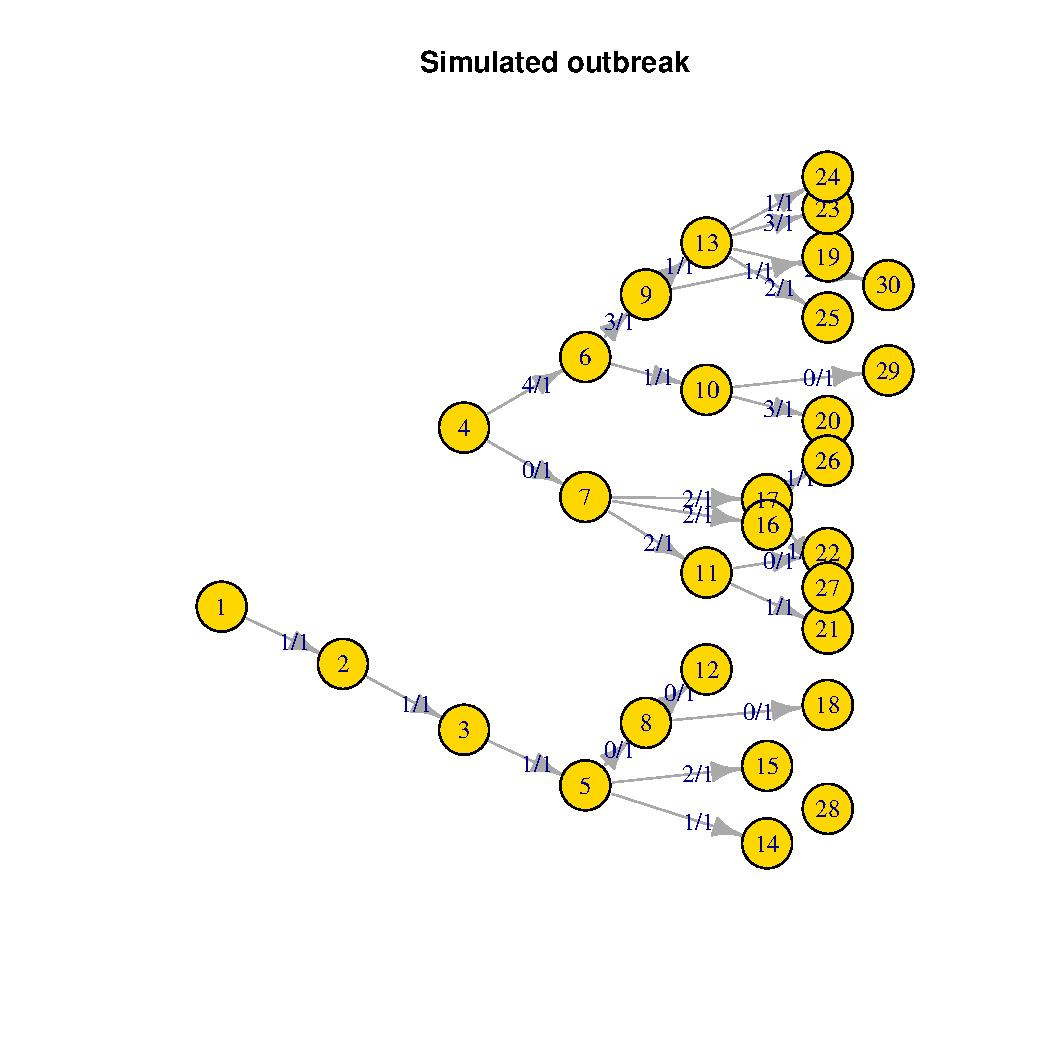
\includegraphics[width=.6\textwidth]{figs/unnamed-chunk-31} 

}


\begin{kframe}\begin{alltt}
\hlkwd{barplot}\hlstd{(w,} \hlkwc{main}\hlstd{=}\hlstr{"Generation time distribution"}\hlstd{,} \hlkwc{ylab}\hlstd{=}\hlstr{"probability"}\hlstd{,} \hlkwc{xlab}\hlstd{=}\hlstr{"days"}\hlstd{,} \hlkwc{names}\hlstd{=}\hlnum{0}\hlopt{:}\hlnum{3}\hlstd{)}
\end{alltt}
\end{kframe}

{\centering 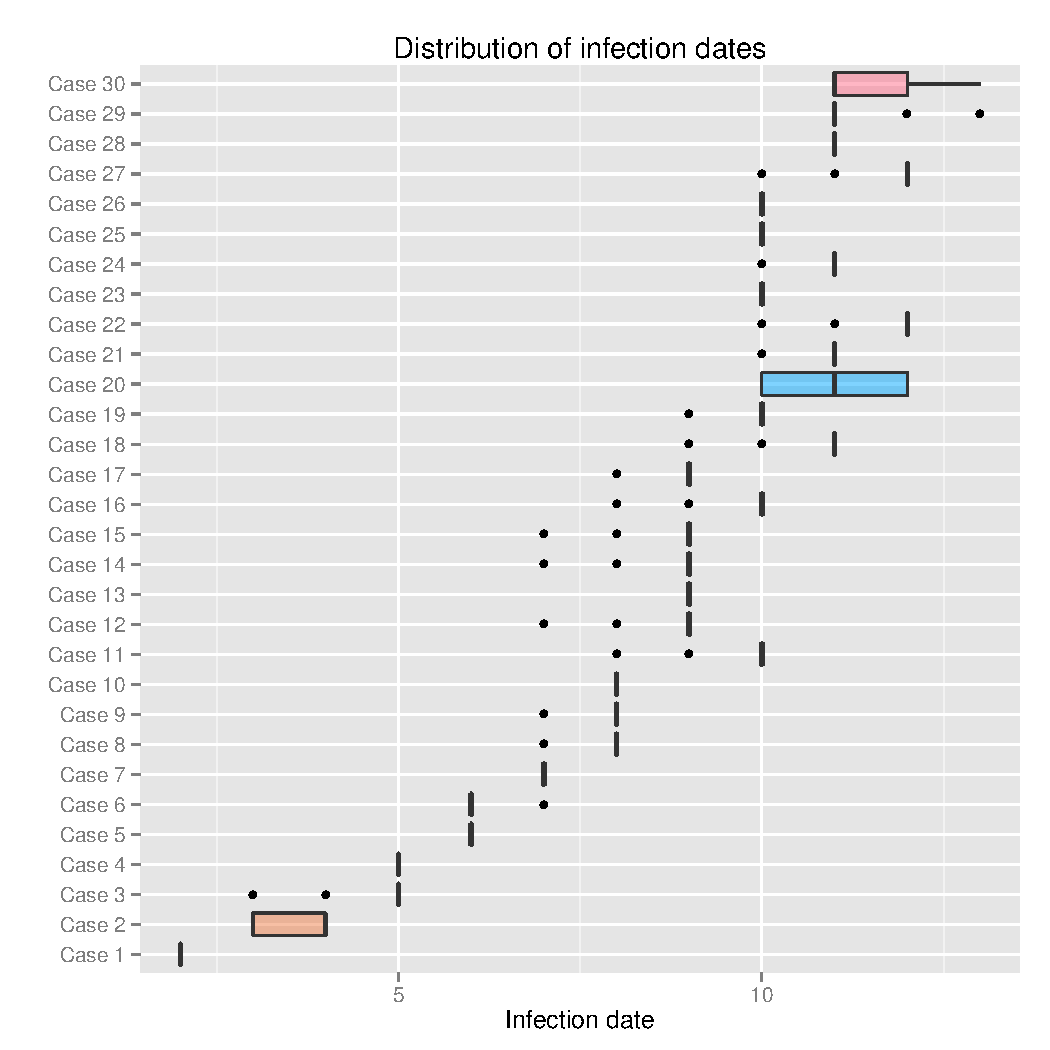
\includegraphics[width=.6\textwidth]{figs/unnamed-chunk-32} 

}



\end{knitrout}



We run \textit{outbreaker} on these data, using the parallel version, and specifying that we want
to run 4 MCMC in parallel and 100,000 chains for each MCMC.
\begin{knitrout}
\definecolor{shadecolor}{rgb}{0.969, 0.969, 0.969}\color{fgcolor}\begin{kframe}
\begin{alltt}
\hlstd{res} \hlkwb{<-}  \hlkwd{outbreaker.parallel}\hlstd{(}\hlkwc{n.runs}\hlstd{=}\hlnum{4}\hlstd{,} \hlkwc{dna}\hlstd{=dat}\hlopt{$}\hlstd{dna,}
                            \hlkwc{dates}\hlstd{=collecDates,}\hlkwc{w.dens}\hlstd{=w,} \hlkwc{n.iter}\hlstd{=}\hlnum{1e5}\hlstd{)}
\end{alltt}
\end{kframe}
\end{knitrout}




\begin{knitrout}
\definecolor{shadecolor}{rgb}{0.969, 0.969, 0.969}\color{fgcolor}\begin{kframe}
\begin{alltt}
\hlkwd{names}\hlstd{(res)}
\end{alltt}
\begin{verbatim}
##  [1] "chains"         "collec.dates"   "w"              "f"             
##  [5] "D"              "idx.dna"        "tune.end"       "find.import"   
##  [9] "burnin"         "find.import.at" "n.runs"         "call"
\end{verbatim}
\end{kframe}
\end{knitrout}


\begin{knitrout}
\definecolor{shadecolor}{rgb}{0.969, 0.969, 0.969}\color{fgcolor}\begin{kframe}
\begin{alltt}
\hlkwd{names}\hlstd{(res}\hlopt{$}\hlstd{chains)}
\end{alltt}
\begin{verbatim}
##   [1] "step"     "post"     "like"     "prior"    "mu1"      "mu2"     
##   [7] "gamma"    "pi"       "spa1"     "spa2"     "Tinf_1"   "Tinf_2"  
##  [13] "Tinf_3"   "Tinf_4"   "Tinf_5"   "Tinf_6"   "Tinf_7"   "Tinf_8"  
##  [19] "Tinf_9"   "Tinf_10"  "Tinf_11"  "Tinf_12"  "Tinf_13"  "Tinf_14" 
##  [25] "Tinf_15"  "Tinf_16"  "Tinf_17"  "Tinf_18"  "Tinf_19"  "Tinf_20" 
##  [31] "Tinf_21"  "Tinf_22"  "Tinf_23"  "Tinf_24"  "Tinf_25"  "Tinf_26" 
##  [37] "Tinf_27"  "Tinf_28"  "Tinf_29"  "Tinf_30"  "alpha_1"  "alpha_2" 
##  [43] "alpha_3"  "alpha_4"  "alpha_5"  "alpha_6"  "alpha_7"  "alpha_8" 
##  [49] "alpha_9"  "alpha_10" "alpha_11" "alpha_12" "alpha_13" "alpha_14"
##  [55] "alpha_15" "alpha_16" "alpha_17" "alpha_18" "alpha_19" "alpha_20"
##  [61] "alpha_21" "alpha_22" "alpha_23" "alpha_24" "alpha_25" "alpha_26"
##  [67] "alpha_27" "alpha_28" "alpha_29" "alpha_30" "kappa_1"  "kappa_2" 
##  [73] "kappa_3"  "kappa_4"  "kappa_5"  "kappa_6"  "kappa_7"  "kappa_8" 
##  [79] "kappa_9"  "kappa_10" "kappa_11" "kappa_12" "kappa_13" "kappa_14"
##  [85] "kappa_15" "kappa_16" "kappa_17" "kappa_18" "kappa_19" "kappa_20"
##  [91] "kappa_21" "kappa_22" "kappa_23" "kappa_24" "kappa_25" "kappa_26"
##  [97] "kappa_27" "kappa_28" "kappa_29" "kappa_30" "run"
\end{verbatim}
\end{kframe}
\end{knitrout}



\begin{knitrout}
\definecolor{shadecolor}{rgb}{0.969, 0.969, 0.969}\color{fgcolor}\begin{kframe}
\begin{alltt}
\hlkwd{class}\hlstd{(res)}
\end{alltt}
\begin{verbatim}
## [1] "list"
\end{verbatim}
\begin{alltt}
\hlkwd{names}\hlstd{(res)}
\end{alltt}
\begin{verbatim}
##  [1] "chains"         "collec.dates"   "w"              "f"             
##  [5] "D"              "idx.dna"        "tune.end"       "find.import"   
##  [9] "burnin"         "find.import.at" "n.runs"         "call"
\end{verbatim}
\end{kframe}
\end{knitrout}

The object \texttt{res} is a list with a number of named items, described in \texttt{?outbreaker}.
The most important one is \texttt{res\$chains}, containing the MCMC outputs:
\begin{knitrout}
\definecolor{shadecolor}{rgb}{0.969, 0.969, 0.969}\color{fgcolor}\begin{kframe}
\begin{alltt}
\hlkwd{class}\hlstd{(res}\hlopt{$}\hlstd{chains)}
\end{alltt}
\begin{verbatim}
## [1] "data.frame"
\end{verbatim}
\begin{alltt}
\hlkwd{dim}\hlstd{(res}\hlopt{$}\hlstd{chains)}
\end{alltt}
\begin{verbatim}
## [1] 804 101
\end{verbatim}
\begin{alltt}
\hlkwd{names}\hlstd{(res}\hlopt{$}\hlstd{chains)}
\end{alltt}
\begin{verbatim}
##   [1] "step"     "post"     "like"     "prior"    "mu1"      "mu2"     
##   [7] "gamma"    "pi"       "spa1"     "spa2"     "Tinf_1"   "Tinf_2"  
##  [13] "Tinf_3"   "Tinf_4"   "Tinf_5"   "Tinf_6"   "Tinf_7"   "Tinf_8"  
##  [19] "Tinf_9"   "Tinf_10"  "Tinf_11"  "Tinf_12"  "Tinf_13"  "Tinf_14" 
##  [25] "Tinf_15"  "Tinf_16"  "Tinf_17"  "Tinf_18"  "Tinf_19"  "Tinf_20" 
##  [31] "Tinf_21"  "Tinf_22"  "Tinf_23"  "Tinf_24"  "Tinf_25"  "Tinf_26" 
##  [37] "Tinf_27"  "Tinf_28"  "Tinf_29"  "Tinf_30"  "alpha_1"  "alpha_2" 
##  [43] "alpha_3"  "alpha_4"  "alpha_5"  "alpha_6"  "alpha_7"  "alpha_8" 
##  [49] "alpha_9"  "alpha_10" "alpha_11" "alpha_12" "alpha_13" "alpha_14"
##  [55] "alpha_15" "alpha_16" "alpha_17" "alpha_18" "alpha_19" "alpha_20"
##  [61] "alpha_21" "alpha_22" "alpha_23" "alpha_24" "alpha_25" "alpha_26"
##  [67] "alpha_27" "alpha_28" "alpha_29" "alpha_30" "kappa_1"  "kappa_2" 
##  [73] "kappa_3"  "kappa_4"  "kappa_5"  "kappa_6"  "kappa_7"  "kappa_8" 
##  [79] "kappa_9"  "kappa_10" "kappa_11" "kappa_12" "kappa_13" "kappa_14"
##  [85] "kappa_15" "kappa_16" "kappa_17" "kappa_18" "kappa_19" "kappa_20"
##  [91] "kappa_21" "kappa_22" "kappa_23" "kappa_24" "kappa_25" "kappa_26"
##  [97] "kappa_27" "kappa_28" "kappa_29" "kappa_30" "run"
\end{verbatim}
\begin{alltt}
\hlstd{res}\hlopt{$}\hlstd{chains[}\hlnum{1}\hlopt{:}\hlnum{10}\hlstd{,}\hlnum{1}\hlopt{:}\hlnum{10}\hlstd{]}
\end{alltt}
\begin{verbatim}
##    step    post    like prior       mu1       mu2 gamma     pi spa1 spa2
## 1     1 -1106.3 -1108.4 2.093 5.000e-05 5.000e-05     1 0.9770    0    0
## 2   500  -468.0  -470.2 2.144 5.021e-05 5.021e-05     1 0.9826    0    0
## 3  1000  -446.9  -448.8 1.909 5.038e-05 5.038e-05     1 0.9572    0    0
## 4  1500  -446.7  -448.9 2.294 5.060e-05 5.060e-05     1 0.9990    0    0
## 5  2000  -446.5  -448.7 2.227 5.087e-05 5.087e-05     1 0.9916    0    0
## 6  2500  -446.6  -448.7 2.147 5.080e-05 5.080e-05     1 0.9829    0    0
## 7  3000  -446.9  -449.1 2.216 5.138e-05 5.138e-05     1 0.9905    0    0
## 8  3500  -448.5  -450.6 2.168 5.078e-05 5.078e-05     1 0.9852    0    0
## 9  4000  -446.8  -449.1 2.233 5.309e-05 5.309e-05     1 0.9923    0    0
## 10 4500  -452.0  -453.8 1.855 5.323e-05 5.323e-05     1 0.9515    0    0
\end{verbatim}
\end{kframe}
\end{knitrout}

The columns of this \texttt{data.frame} store the following outputs:
\begin{itemize}
  \item \texttt{step}: the MCMC iteration of the sample
  \item \texttt{post/like/prior}: log values for posterior, likelihood, and prior densities
  \item \texttt{mu1}: in mutation model 1, mutation rate; otherwise, the rate of transitions, per site and generation
  \item \texttt{mu2}: in mutation model 1, mutation rate (mu1=mu2); otherwise, the rate of transversions, per site and generation
  \item \texttt{gamma}: the ratio between transversions and transitions ($\mu_2 / \mu_1$)
  \item \texttt{pi}: the proportion of the transmission tree sampled
  \item \texttt{Tinf\_[}\textit{number}\texttt{]}: dates of infection
  \item \texttt{alpha\_[}\textit{number}\texttt{]}: the index of the ancestral cases (infectors)
  \item \texttt{kappa\_[}\textit{number}\texttt{]}: the number of generations between cases and
    their most recent sampled ancestor (here, fixed to 1)
  \item \texttt{run}: for parallel runs, the index of the run.
\end{itemize}

We shall see how this information can be used, visualized and interpreted over the following sections.




%%%%%%%%%%%%%%%%%%%%%%%%%%%%%%%%%%%%%%%%%%%%%%%%%%%%
\subsection{Assessing convergence and determining the burnin}
%%%%%%%%%%%%%%%%%%%%%%%%%%%%%%%%%%%%%%%%%%%%%%%%%%%%

A MCMC is said to converge when it reaches a stationary state, i.e. its distributional properties are
constant over time (mean and variance don't depend on which window of the MCMC you consider).
Convergence of the chains is best assessed by comparing parallel runs.
This can be done using \texttt{plotChains}, which we to visualize the trace of the log-posterior
values of the model:
\begin{knitrout}
\definecolor{shadecolor}{rgb}{0.969, 0.969, 0.969}\color{fgcolor}\begin{kframe}
\begin{alltt}
\hlkwd{plotChains}\hlstd{(res,} \hlkwc{main}\hlstd{=}\hlstr{"Trace of log-posterior values"}\hlstd{)}
\end{alltt}
\end{kframe}

{\centering 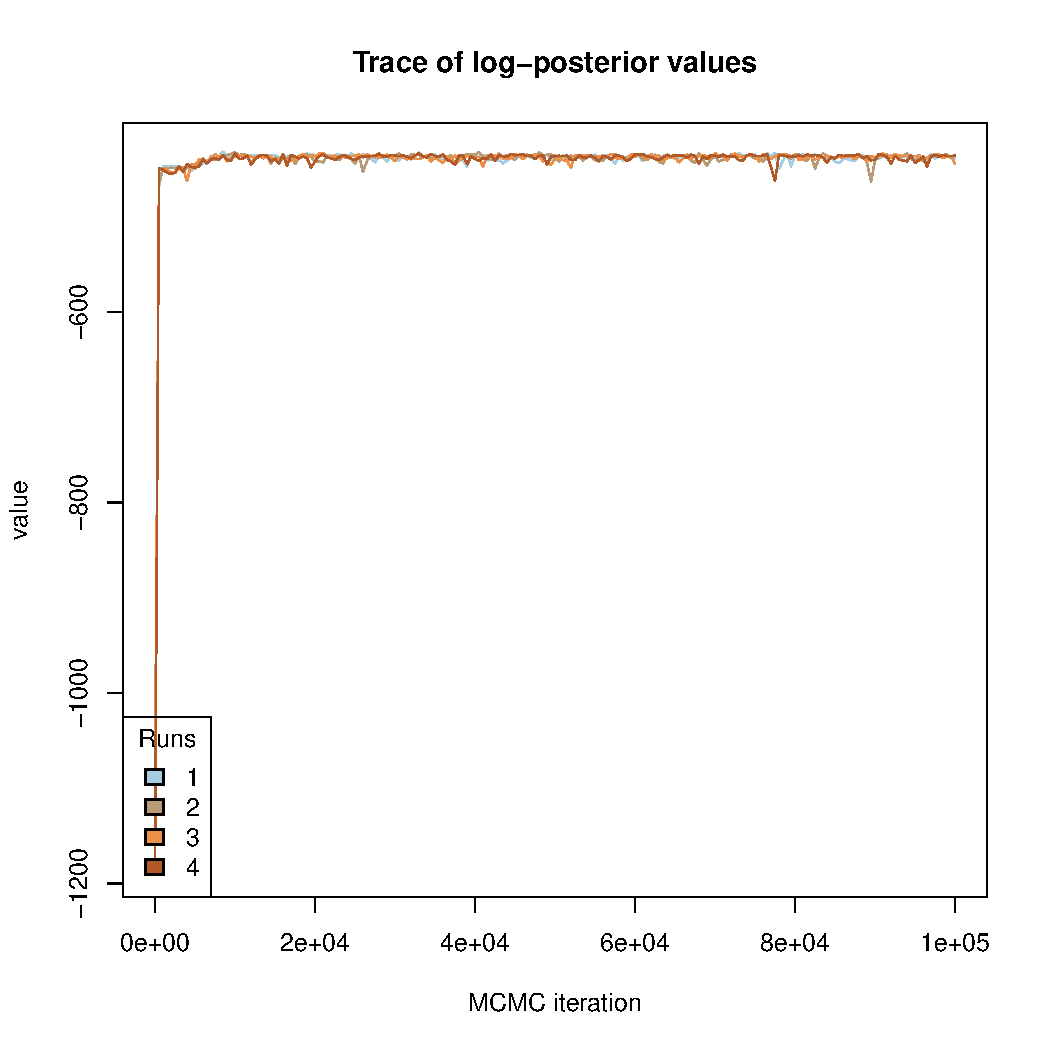
\includegraphics[width=.6\textwidth]{figs/unnamed-chunk-10} 

}



\end{knitrout}


\noindent We set the burnin to a conservative 20,000 steps, and plot the MCMC output as trace and as densities:
\begin{knitrout}
\definecolor{shadecolor}{rgb}{0.969, 0.969, 0.969}\color{fgcolor}\begin{kframe}
\begin{alltt}
\hlkwd{plotChains}\hlstd{(res,} \hlkwc{main}\hlstd{=}\hlstr{"Trace of log-posterior values \textbackslash{}n(burnin removed)"}\hlstd{,}
           \hlkwc{burnin}\hlstd{=}\hlnum{2e4}\hlstd{)}
\end{alltt}
\end{kframe}

{\centering 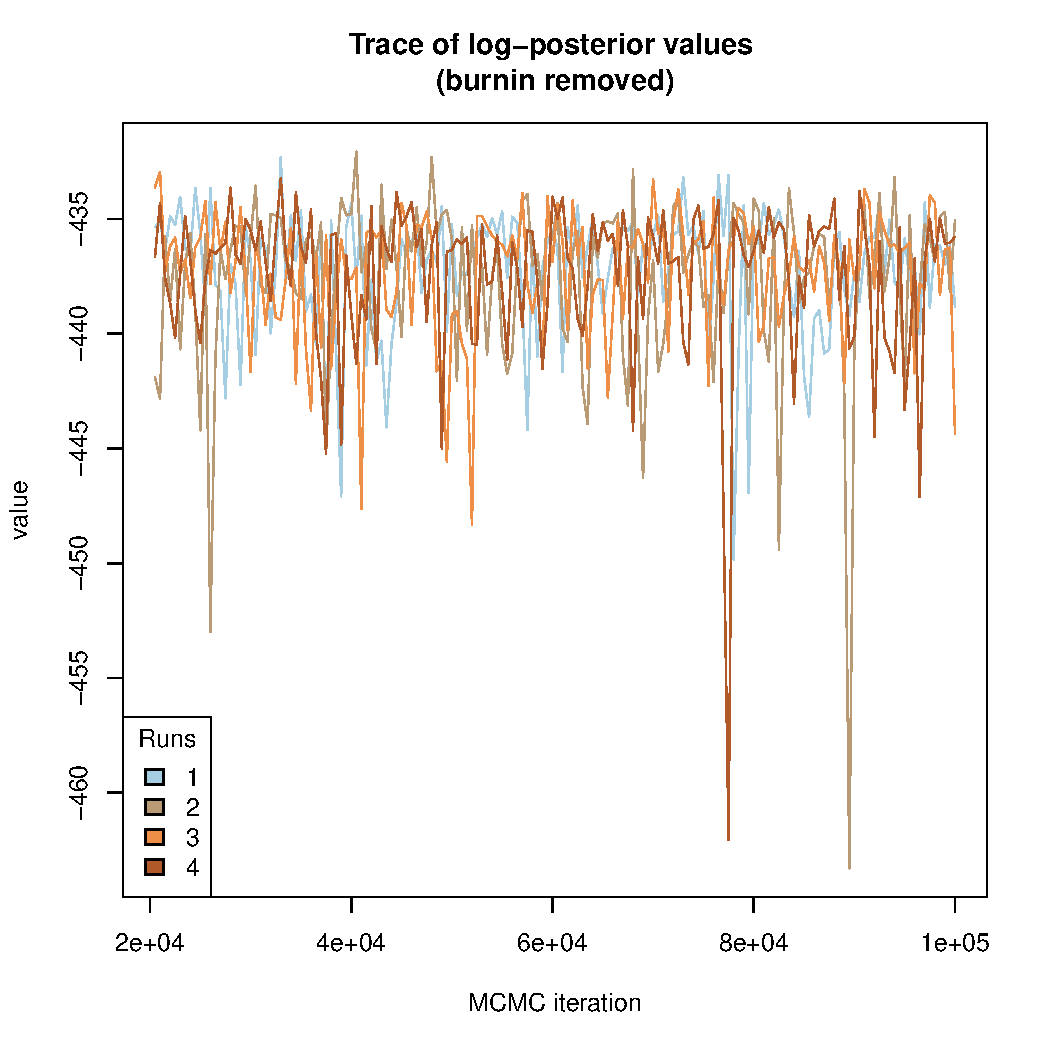
\includegraphics[width=.6\textwidth]{figs/unnamed-chunk-111} 

}


\begin{kframe}\begin{alltt}
\hlkwd{plotChains}\hlstd{(res,} \hlkwc{main}\hlstd{=}\hlstr{"Density log-posterior values \textbackslash{}n(burnin removed)"}\hlstd{,}
           \hlkwc{burnin}\hlstd{=}\hlnum{2e4}\hlstd{,} \hlkwc{type}\hlstd{=}\hlstr{"dens"}\hlstd{)}
\end{alltt}
\end{kframe}

{\centering 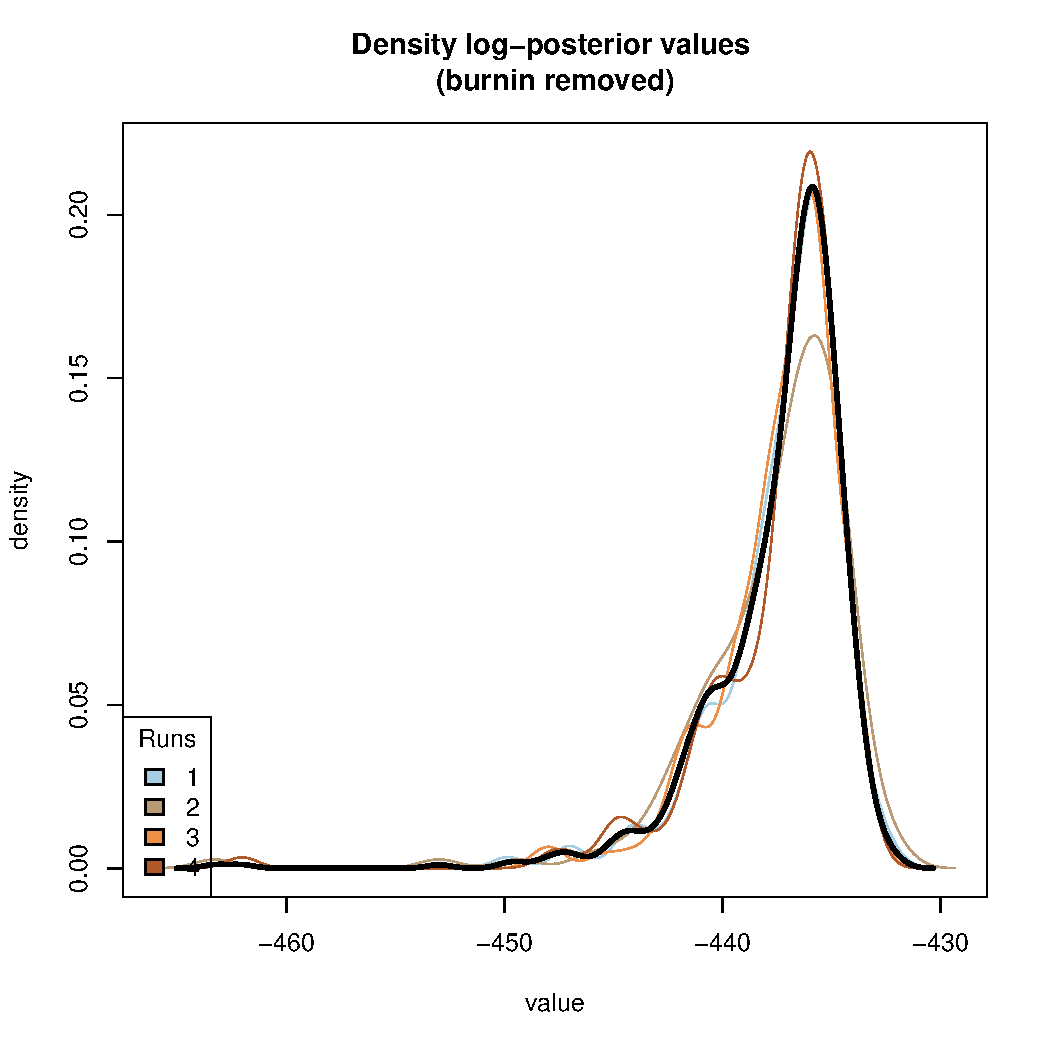
\includegraphics[width=.6\textwidth]{figs/unnamed-chunk-112} 

}



\end{knitrout}

Here, all four runs have sampled from the same distribution, confirming convergence of the MCMCs.
Note that this can also be tested using a simple ANOVA, which we use to check that log-posterior
values do no differ from one run to another:
\begin{knitrout}
\definecolor{shadecolor}{rgb}{0.969, 0.969, 0.969}\color{fgcolor}\begin{kframe}
\begin{alltt}
\hlkwd{anova}\hlstd{(}\hlkwd{lm}\hlstd{(post}\hlopt{~}\hlstd{run,} \hlkwc{data}\hlstd{=res}\hlopt{$}\hlstd{chains[res}\hlopt{$}\hlstd{chains}\hlopt{$}\hlstd{step}\hlopt{>}\hlnum{2e4}\hlstd{,]))}
\end{alltt}
\begin{verbatim}
## Analysis of Variance Table
## 
## Response: post
##            Df Sum Sq Mean Sq F value Pr(>F)
## run         1      0     0.3    0.03   0.86
## Residuals 638   6387    10.0
\end{verbatim}
\end{kframe}
\end{knitrout}



These graphs can be slightly improved by using \textit{ggplot2}.
We first load the package, and make sure that \texttt{run} is treated as a \texttt{factor}:
\begin{knitrout}
\definecolor{shadecolor}{rgb}{0.969, 0.969, 0.969}\color{fgcolor}\begin{kframe}
\begin{alltt}
\hlkwd{library}\hlstd{(ggplot2)}
\hlkwd{library}\hlstd{(reshape2)}
\hlstd{x} \hlkwb{<-} \hlstd{res}\hlopt{$}\hlstd{chains}
\hlstd{x}\hlopt{$}\hlstd{run} \hlkwb{<-} \hlkwd{factor}\hlstd{(x}\hlopt{$}\hlstd{run)}
\end{alltt}
\end{kframe}
\end{knitrout}

The basic plot of the log-posterior trace is obtained by:
\begin{knitrout}
\definecolor{shadecolor}{rgb}{0.969, 0.969, 0.969}\color{fgcolor}\begin{kframe}
\begin{alltt}
\hlstd{p} \hlkwb{<-} \hlkwd{ggplot}\hlstd{(x,} \hlkwd{aes}\hlstd{(}\hlkwc{x}\hlstd{=step))} \hlopt{+}
    \hlkwd{geom_line}\hlstd{(}\hlkwd{aes}\hlstd{(}\hlkwc{y}\hlstd{=post,} \hlkwc{colour}\hlstd{=run))} \hlopt{+}
    \hlkwd{labs}\hlstd{(}\hlkwc{title}\hlstd{=}\hlstr{"Trace of log-posterior"}\hlstd{,} \hlkwc{y}\hlstd{=}\hlstr{"log-posterior"}\hlstd{)}
\hlstd{p}
\end{alltt}
\end{kframe}

{\centering 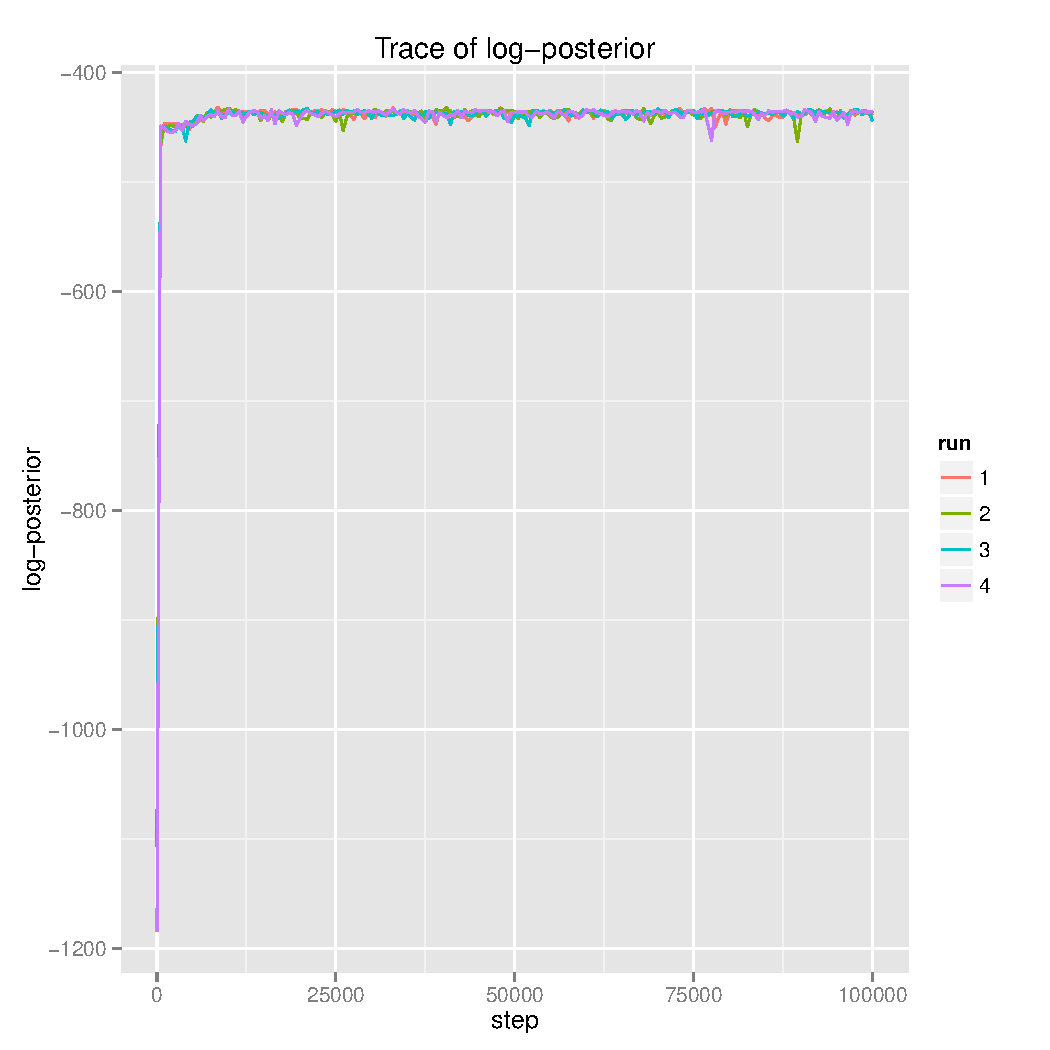
\includegraphics[width=.6\textwidth]{figs/unnamed-chunk-14} 

}



\end{knitrout}


The version without the burnin is:
\begin{knitrout}
\definecolor{shadecolor}{rgb}{0.969, 0.969, 0.969}\color{fgcolor}\begin{kframe}
\begin{alltt}
\hlstd{p} \hlkwb{<-} \hlkwd{ggplot}\hlstd{(x[x}\hlopt{$}\hlstd{step}\hlopt{>}\hlnum{2e4}\hlstd{,],} \hlkwd{aes}\hlstd{(}\hlkwc{x}\hlstd{=step))} \hlopt{+}
    \hlkwd{geom_line}\hlstd{(}\hlkwd{aes}\hlstd{(}\hlkwc{y}\hlstd{=post,} \hlkwc{colour}\hlstd{=run))} \hlopt{+}
    \hlkwd{labs}\hlstd{(}\hlkwc{title}\hlstd{=}\hlstr{"Trace of log-posterior"}\hlstd{,} \hlkwc{y}\hlstd{=}\hlstr{"log-posterior"}\hlstd{)}
\hlstd{p}
\end{alltt}
\end{kframe}

{\centering 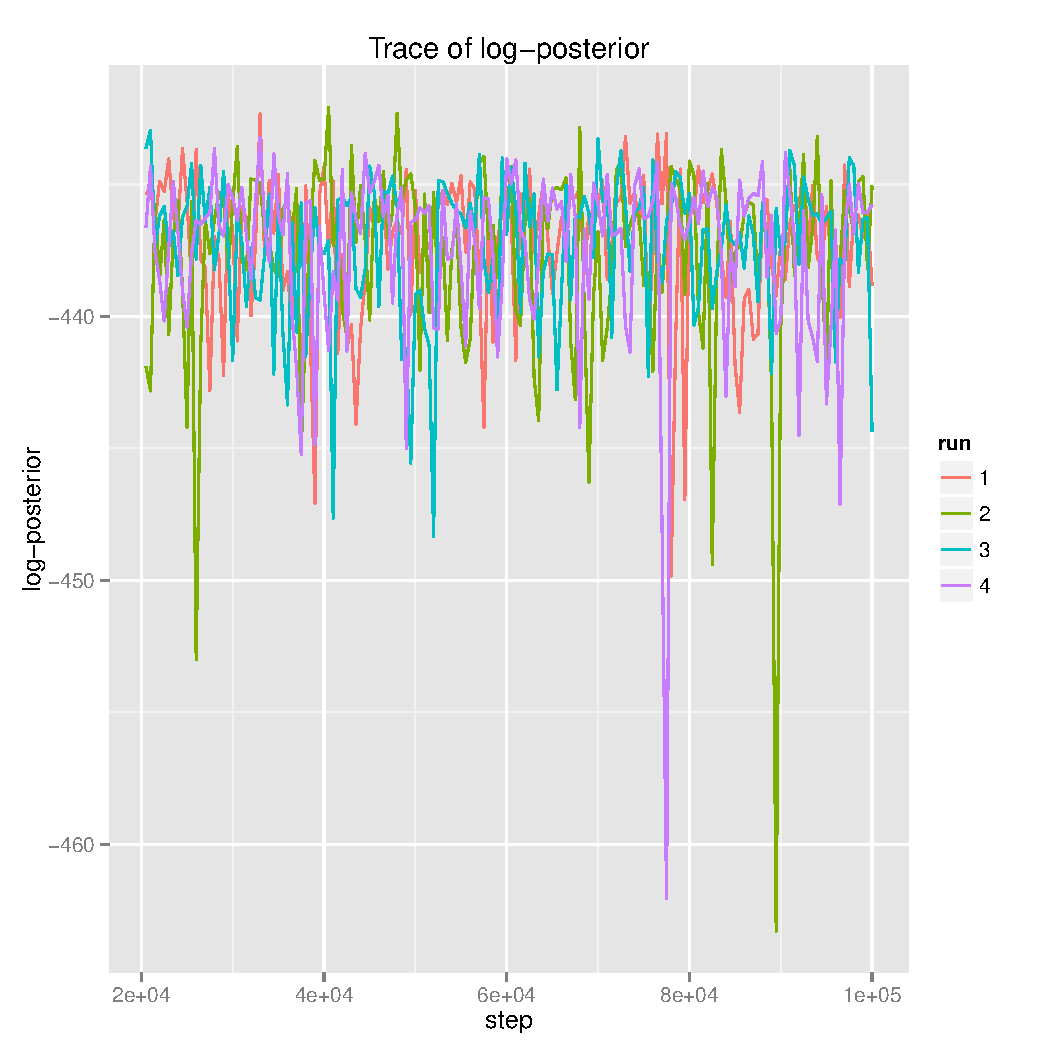
\includegraphics[width=.6\textwidth]{figs/unnamed-chunk-15} 

}



\end{knitrout}


A model of the mean can be added easily:
\begin{knitrout}
\definecolor{shadecolor}{rgb}{0.969, 0.969, 0.969}\color{fgcolor}\begin{kframe}
\begin{alltt}
\hlstd{p} \hlopt{+} \hlkwd{geom_smooth}\hlstd{(}\hlkwd{aes}\hlstd{(}\hlkwc{y}\hlstd{=post))}
\end{alltt}


{\ttfamily\noindent\itshape\color{messagecolor}{\#\# geom\_smooth: method="{}auto"{} and size of largest group is <1000, so using loess. Use 'method = x' to change the smoothing method.}}\end{kframe}

{\centering 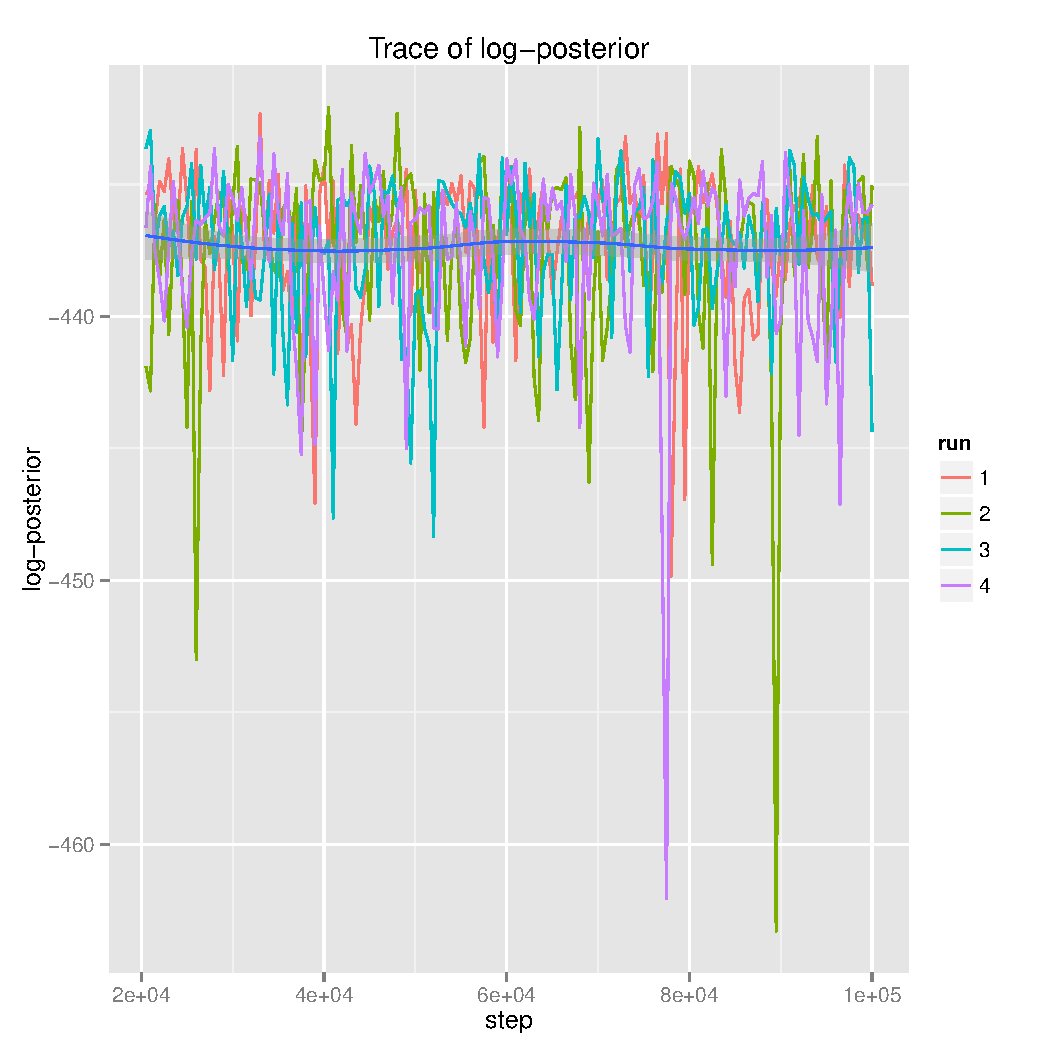
\includegraphics[width=.6\textwidth]{figs/unnamed-chunk-16} 

}



\end{knitrout}


\textit{ggplot2} is also pretty good for plotting distributions.
Here is an example using 1-dimensional density estimation:
\begin{knitrout}
\definecolor{shadecolor}{rgb}{0.969, 0.969, 0.969}\color{fgcolor}\begin{kframe}
\begin{alltt}
\hlstd{p} \hlkwb{<-} \hlkwd{ggplot}\hlstd{(}\hlkwc{data}\hlstd{=x)} \hlopt{+} \hlkwd{labs}\hlstd{(}\hlkwc{title}\hlstd{=}\hlstr{"Distribution of log-posterior values"}\hlstd{,} \hlkwc{x}\hlstd{=}\hlstr{"log-posterior"}\hlstd{)} \hlopt{+}
    \hlkwd{scale_x_continuous}\hlstd{(}\hlkwc{limits}\hlstd{=}\hlkwd{c}\hlstd{(}\hlopt{-}\hlnum{460}\hlstd{,}\hlopt{-}\hlnum{430}\hlstd{))}
\hlstd{p} \hlopt{+} \hlkwd{geom_density}\hlstd{(}\hlkwd{aes}\hlstd{(}\hlkwc{x}\hlstd{=post,} \hlkwc{fill}\hlstd{=run),} \hlkwc{alpha}\hlstd{=}\hlnum{.3}\hlstd{,} \hlkwc{colour}\hlstd{=}\hlnum{NA}\hlstd{)} \hlopt{+}
    \hlkwd{geom_density}\hlstd{(}\hlkwd{aes}\hlstd{(}\hlkwc{x}\hlstd{=post),} \hlkwc{size}\hlstd{=}\hlnum{1}\hlstd{,} \hlkwc{colour}\hlstd{=}\hlstr{"black"}\hlstd{,} \hlkwc{shape}\hlstd{=}\hlnum{2}\hlstd{,} \hlkwc{alpha}\hlstd{=}\hlnum{.8}\hlstd{)}
\end{alltt}
\end{kframe}

{\centering 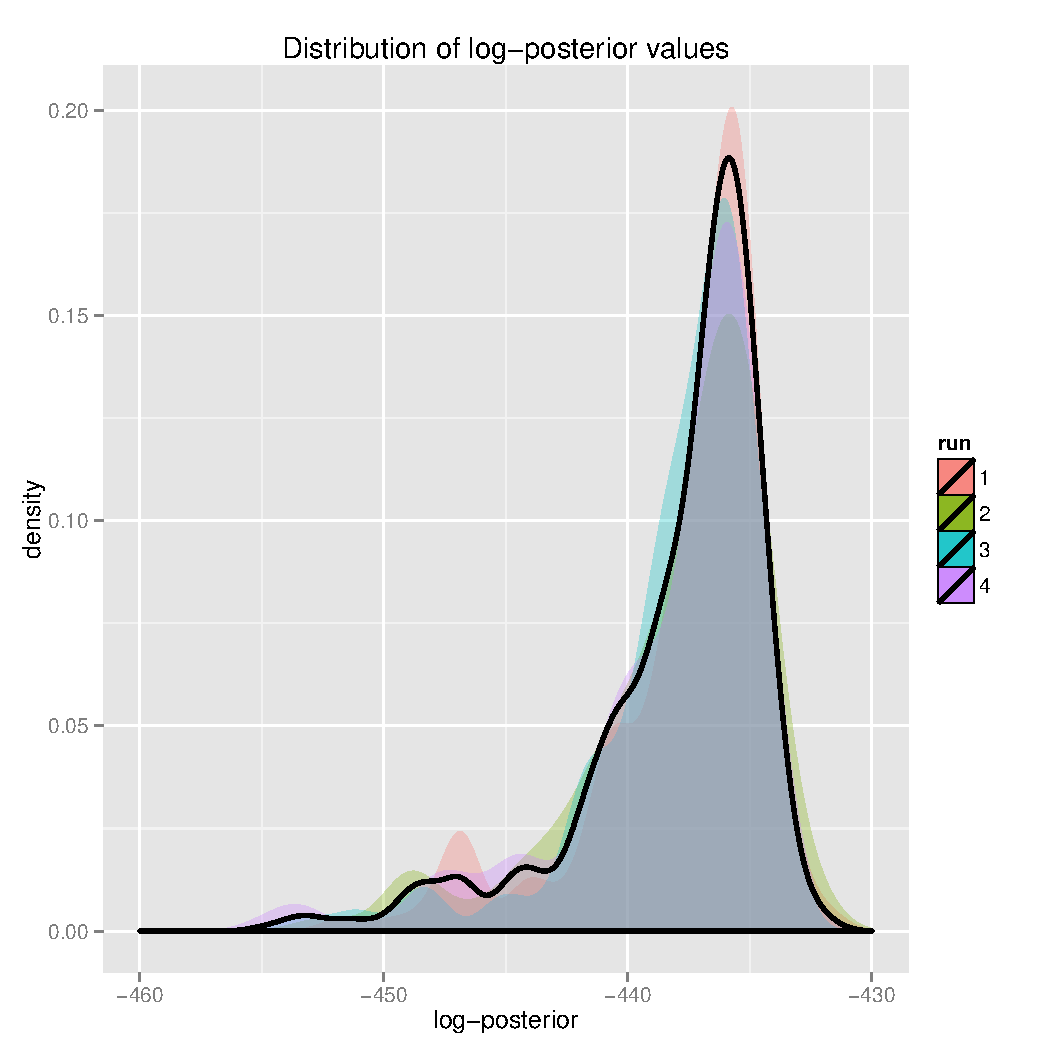
\includegraphics[width=.6\textwidth]{figs/unnamed-chunk-17} 

}



\end{knitrout}

and another version using histograms:
\begin{knitrout}
\definecolor{shadecolor}{rgb}{0.969, 0.969, 0.969}\color{fgcolor}\begin{kframe}
\begin{alltt}
\hlstd{p} \hlopt{+} \hlkwd{geom_histogram}\hlstd{(}\hlkwd{aes}\hlstd{(}\hlkwc{x}\hlstd{=post,} \hlkwc{fill}\hlstd{=run,} \hlkwc{y}\hlstd{=..density..),} \hlkwc{alpha}\hlstd{=}\hlnum{.7}\hlstd{,} \hlkwc{colour}\hlstd{=}\hlnum{NA}\hlstd{,} \hlkwc{position}\hlstd{=}\hlstr{"dodge"}\hlstd{)} \hlopt{+}
    \hlkwd{geom_density}\hlstd{(}\hlkwd{aes}\hlstd{(}\hlkwc{x}\hlstd{=post),} \hlkwc{size}\hlstd{=}\hlnum{1}\hlstd{,} \hlkwc{colour}\hlstd{=}\hlstr{"black"}\hlstd{,} \hlkwc{shape}\hlstd{=}\hlnum{2}\hlstd{,} \hlkwc{alpha}\hlstd{=}\hlnum{.8}\hlstd{)}
\end{alltt}


{\ttfamily\noindent\itshape\color{messagecolor}{\#\# stat\_bin: binwidth defaulted to range/30. Use 'binwidth = x' to adjust this.}}\end{kframe}

{\centering 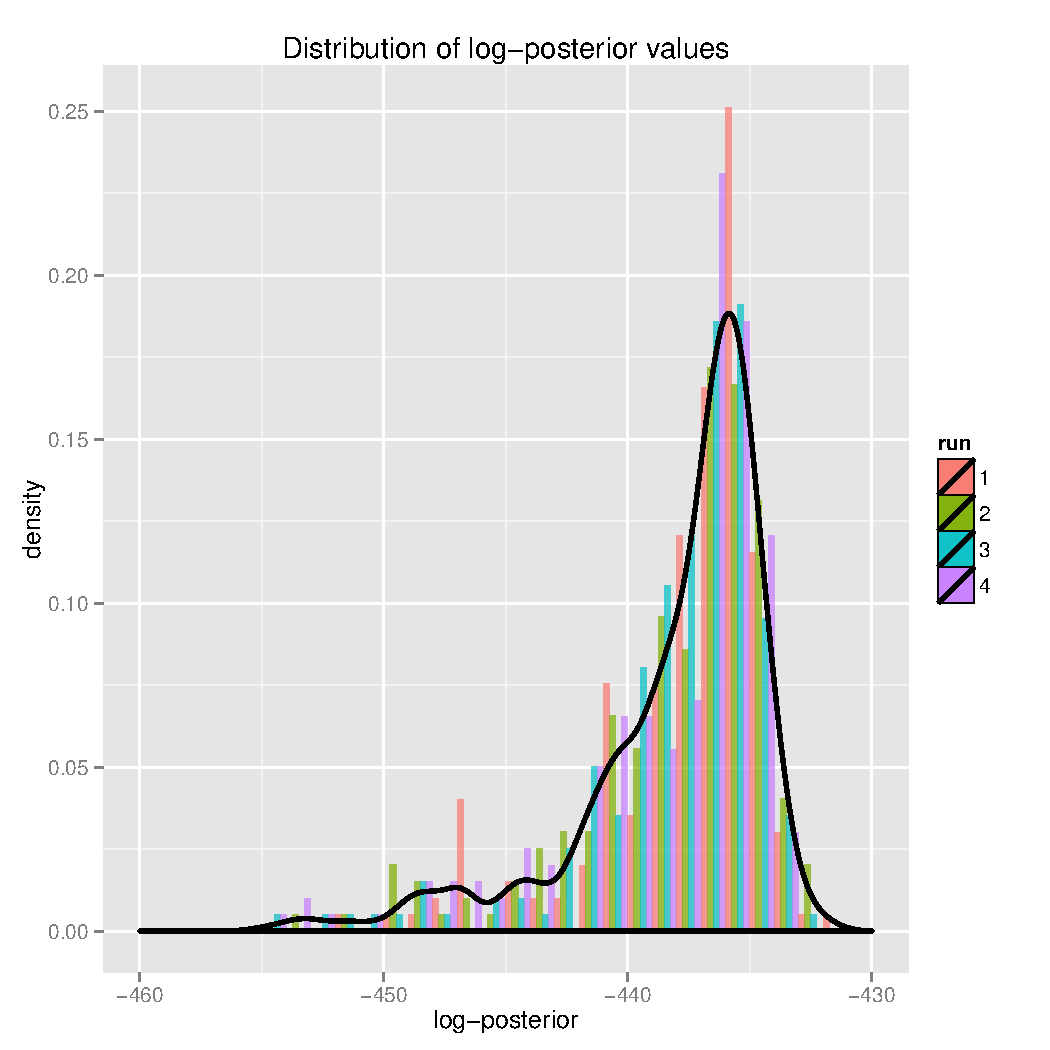
\includegraphics[width=.6\textwidth]{figs/unnamed-chunk-18} 

}



\end{knitrout}







%%%%%%%%%%%%%%%%%%%%%%%%%%%%%%%%%%%%%%%%%%%%%%%%%%%%
%%%%%%%%%%%%%%%%%%%%%%%%%%%%%%%%%%%%%%%%%%%%%%%%%%%%
\section{Interpreting the results}
%%%%%%%%%%%%%%%%%%%%%%%%%%%%%%%%%%%%%%%%%%%%%%%%%%%%
%%%%%%%%%%%%%%%%%%%%%%%%%%%%%%%%%%%%%%%%%%%%%%%%%%%%

\textit{outbreaker} can provide information on:
\begin{itemize}
  \item the transmission tree (``who infected whom''); ancestry for case $i$ is noted $\alpha_i$
  \item the dates of infection; for case $i$, noted $T^{inf}_i$
  \item the mutation rate per generation of infection ($\mu$)
  \item the proportion of the outbreak sampled ($\pi$)
  \item effective reproduction numbers over time or at an individual level $^\dagger$
  \item incidence curves $^\dagger$
  \item the mutation rate per unit of time $^\dagger$
\end{itemize}
Items indicated with a $^\dagger$ are not explicitely modelled by \textit{outbreaker}, but can be derived from the
posterior samples of trees and parameters.



%%%%%%%%%%%%%%%%%%%%%%%%%%%%%%%%%%%%%%%%%%%%%%%%%%%%
\subsection{Visualizing reconstructed transmission trees}
%%%%%%%%%%%%%%%%%%%%%%%%%%%%%%%%%%%%%%%%%%%%%%%%%%%%

\textit{outbreaker} being a Bayesian approach, it does not return a single tree, but a distribution
of plausible transmission trees.
A set of ancestries can be visualized by \texttt{transGraph}
\begin{knitrout}
\definecolor{shadecolor}{rgb}{0.969, 0.969, 0.969}\color{fgcolor}\begin{kframe}
\begin{alltt}
\hlkwd{library}\hlstd{(igraph)}
\hlkwd{library}\hlstd{(adegenet)}
\end{alltt}
\end{kframe}
\end{knitrout}

\begin{knitrout}
\definecolor{shadecolor}{rgb}{0.969, 0.969, 0.969}\color{fgcolor}\begin{kframe}
\begin{alltt}
\hlstd{g} \hlkwb{<-} \hlkwd{transGraph}\hlstd{(res,} \hlkwc{thres}\hlstd{=}\hlnum{0}\hlstd{)}
\end{alltt}
\end{kframe}

{\centering 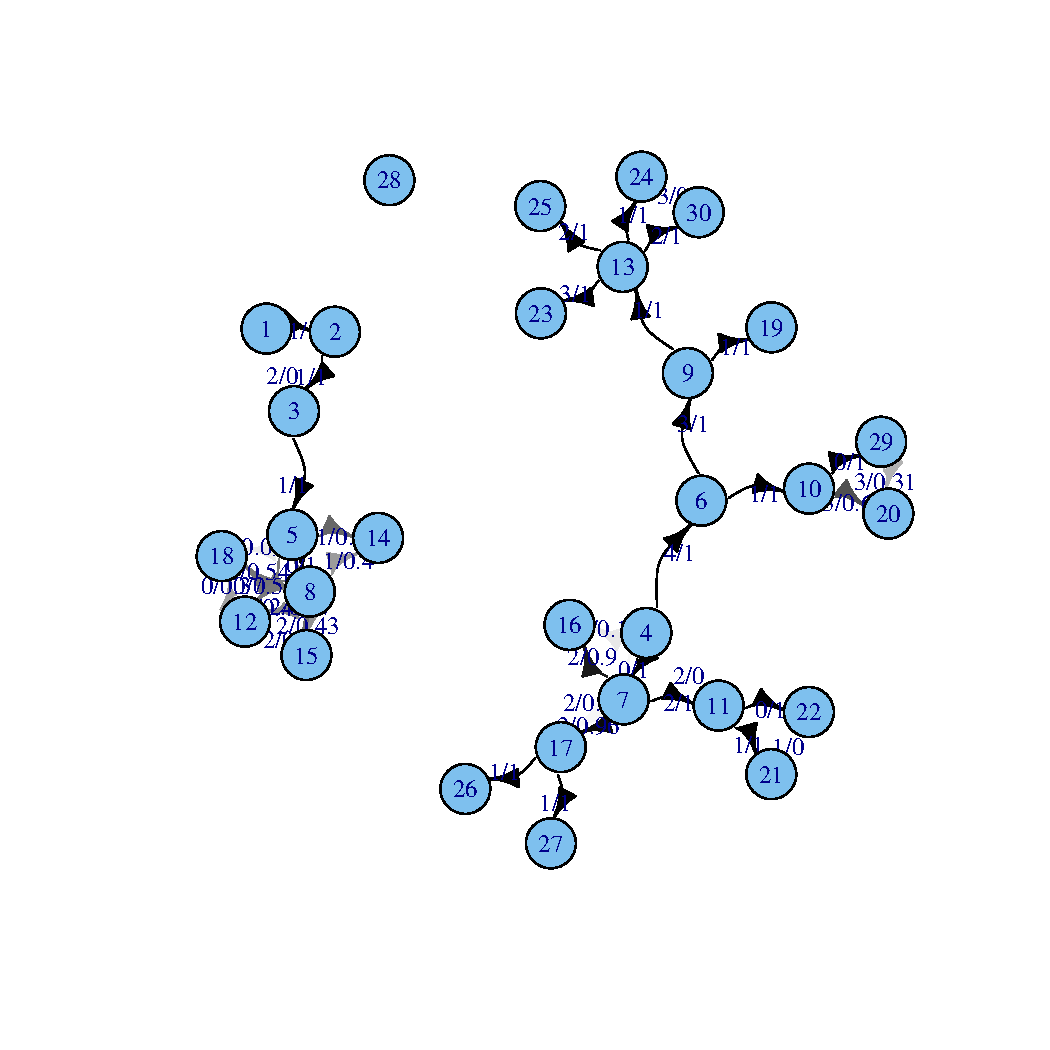
\includegraphics[width=.6\textwidth]{figs/unnamed-chunk-20} 

}



\end{knitrout}

Annotations represent the number of mutations for the ancestries, and their support (frequency in
the posterior samples).
Note that this function returns an \textit{igraph} object, which can be used for further plotting
and customization:
\begin{knitrout}
\definecolor{shadecolor}{rgb}{0.969, 0.969, 0.969}\color{fgcolor}\begin{kframe}
\begin{alltt}
\hlstd{g}
\end{alltt}
\begin{verbatim}
## IGRAPH DN-- 30 40 -- 
## + attr: name (v/c), dates (v/n), label (v/n), color (e/c), support
##   (e/n), curved (e/x), nb.mut (e/n), label (e/c)
\end{verbatim}
\begin{alltt}
\hlkwd{plot}\hlstd{(g,} \hlkwc{layout}\hlstd{=layout.circle,} \hlkwc{edge.curved}\hlstd{=}\hlnum{FALSE}\hlstd{,} \hlkwc{vertex.color}\hlstd{=}\hlkwd{funky}\hlstd{(}\hlnum{30}\hlstd{))}
\end{alltt}
\end{kframe}

{\centering 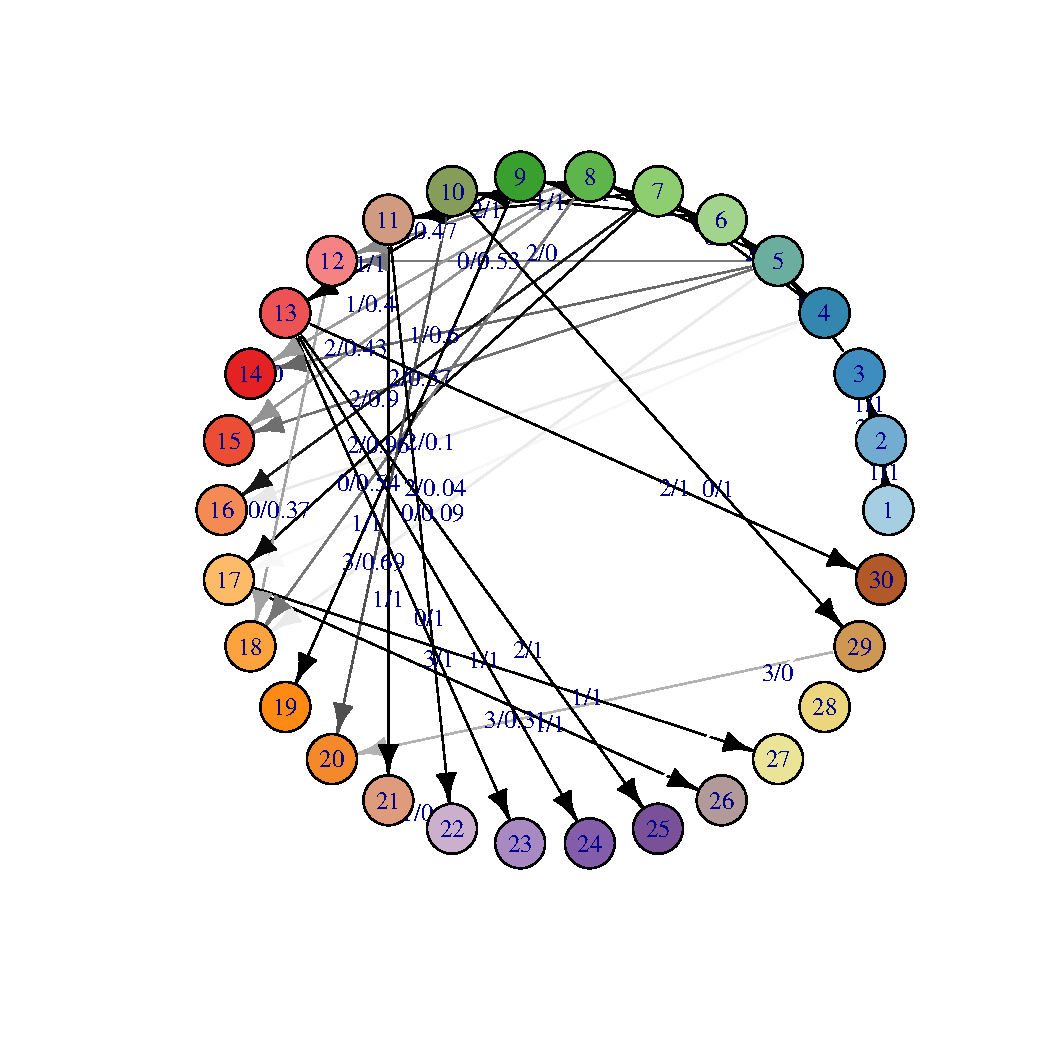
\includegraphics[width=.6\textwidth]{figs/unnamed-chunk-21} 

}



\end{knitrout}

see \texttt{?plot.igraph} and \texttt{igraph.plotting} for more information on how to customize
these graphics.
We illustrate some possibilities below:
\begin{knitrout}
\definecolor{shadecolor}{rgb}{0.969, 0.969, 0.969}\color{fgcolor}\begin{kframe}
\begin{alltt}
\hlstd{g} \hlkwb{<-} \hlkwd{transGraph}\hlstd{(res,} \hlkwc{thres}\hlstd{=}\hlnum{0.5}\hlstd{,} \hlkwc{annot}\hlstd{=}\hlstr{""}\hlstd{)}
\end{alltt}
\end{kframe}

{\centering 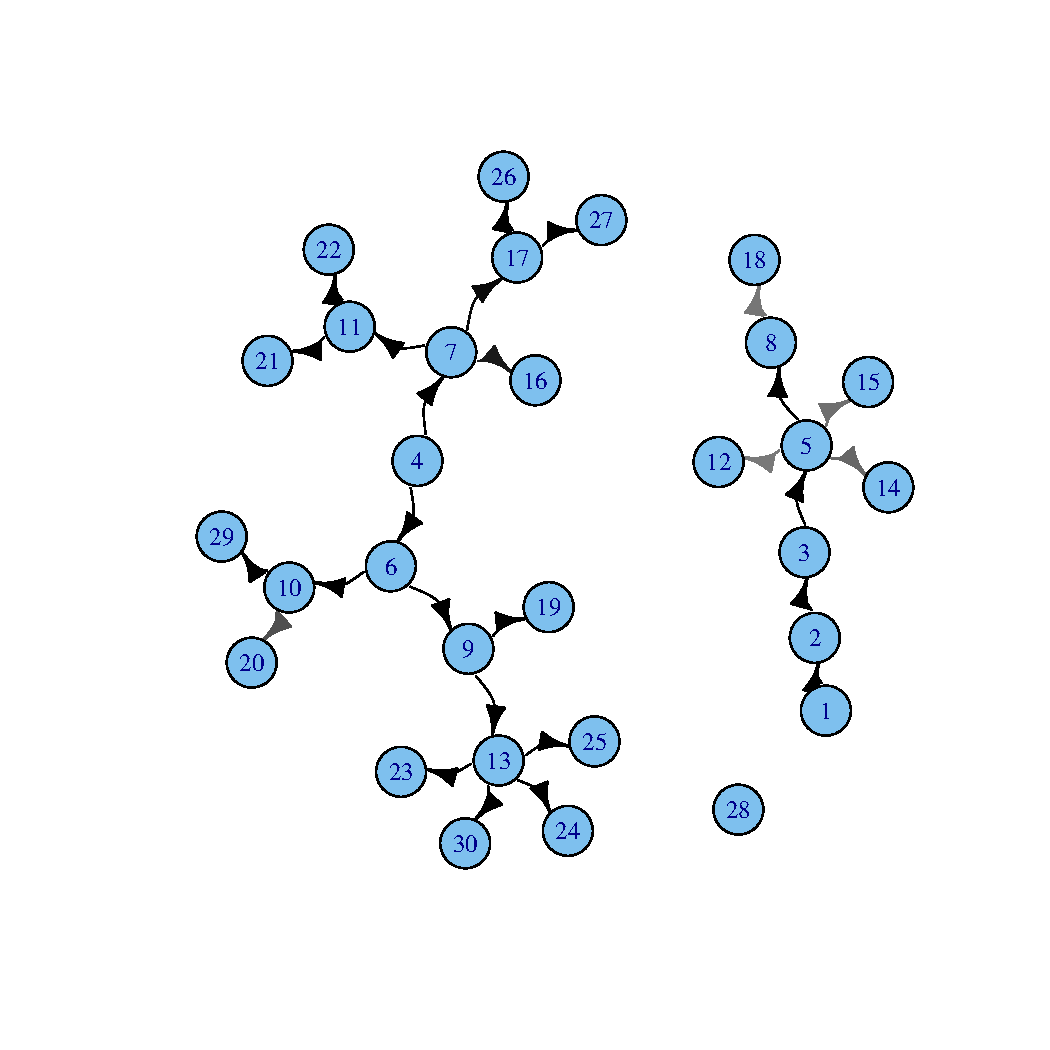
\includegraphics[width=.6\textwidth]{figs/unnamed-chunk-221} 

}


\begin{kframe}\begin{alltt}
\hlstd{edge.colors} \hlkwb{<-} \hlkwd{funky}\hlstd{(}\hlnum{30}\hlstd{)[}\hlkwd{as.numeric}\hlstd{(}\hlkwd{get.edgelist}\hlstd{(g)[,}\hlnum{1}\hlstd{])]}
\hlkwd{plot}\hlstd{(g,} \hlkwc{layout}\hlstd{=layout.circle,} \hlkwc{edge.curved}\hlstd{=}\hlnum{FALSE}\hlstd{,} \hlkwc{vertex.color}\hlstd{=}\hlkwd{funky}\hlstd{(}\hlnum{30}\hlstd{),}
     \hlkwc{edge.color}\hlstd{=edge.colors)}
\hlkwd{title}\hlstd{(}\hlstr{"Ancestries with support >50% - circular graph"}\hlstd{)}
\end{alltt}
\end{kframe}

{\centering 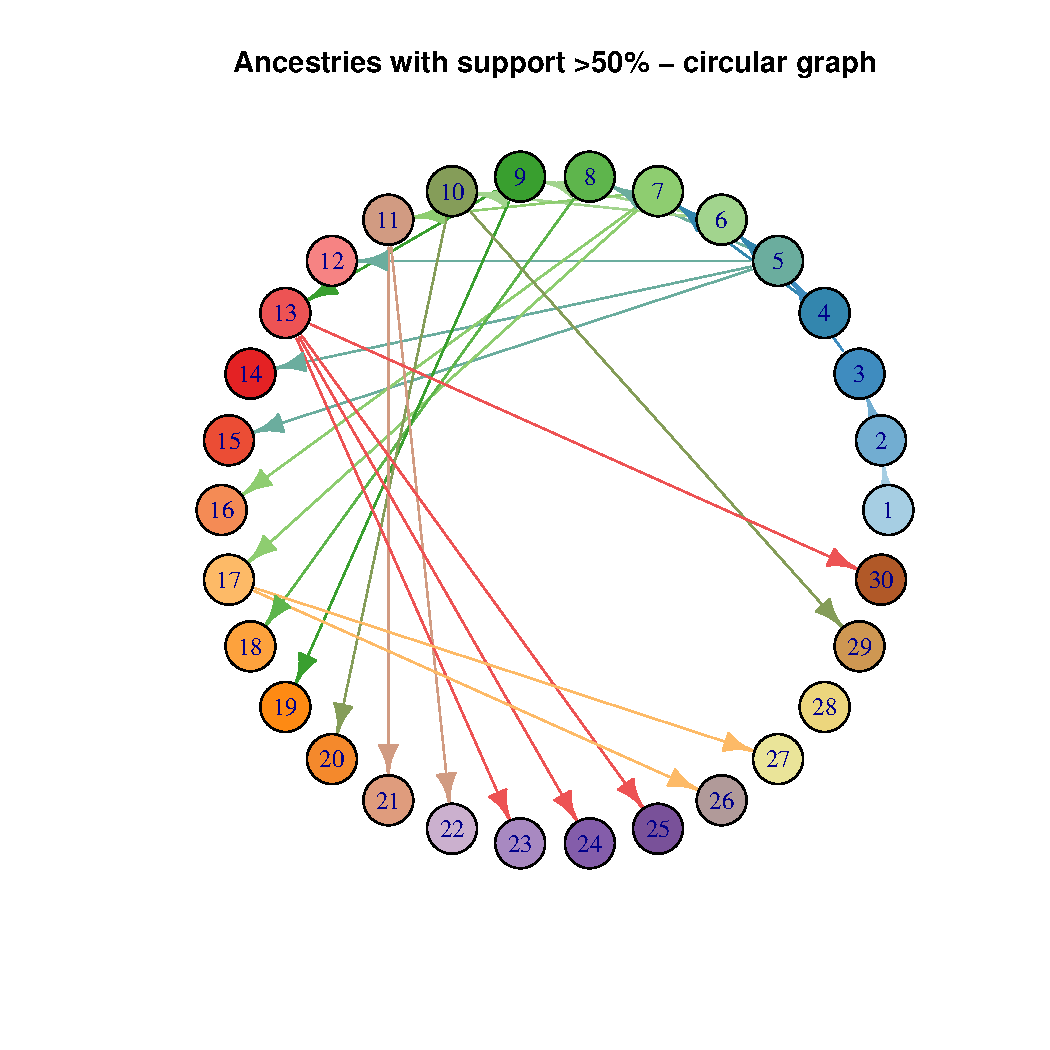
\includegraphics[width=.6\textwidth]{figs/unnamed-chunk-222} 

}


\begin{kframe}\begin{alltt}
\hlkwd{plot}\hlstd{(g,} \hlkwc{layout}\hlstd{=layout.auto,} \hlkwc{edge.curved}\hlstd{=}\hlnum{FALSE}\hlstd{,} \hlkwc{vertex.color}\hlstd{=}\hlkwd{funky}\hlstd{(}\hlnum{30}\hlstd{),}
     \hlkwc{edge.color}\hlstd{=edge.colors)}
\hlkwd{title}\hlstd{(}\hlstr{"Ancestries with support >50% - other layout"}\hlstd{)}
\end{alltt}
\end{kframe}

{\centering 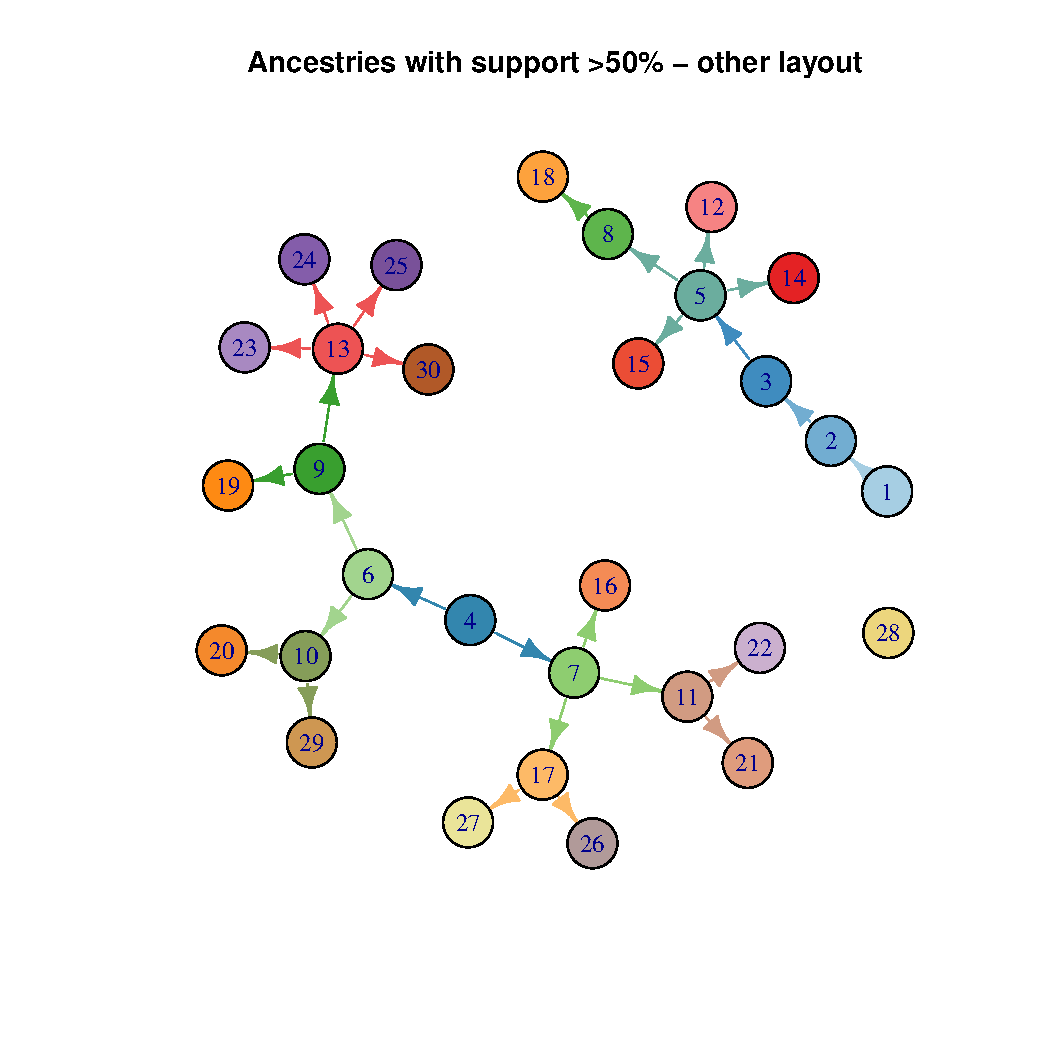
\includegraphics[width=.6\textwidth]{figs/unnamed-chunk-223} 

}



\end{knitrout}


Here we ensure that cases with higher reproduction numbers look bigger:
\begin{knitrout}
\definecolor{shadecolor}{rgb}{0.969, 0.969, 0.969}\color{fgcolor}\begin{kframe}
\begin{alltt}
\hlstd{case.size} \hlkwb{<-} \hlnum{10}\hlopt{+}\hlkwd{apply}\hlstd{(}\hlkwd{get.R}\hlstd{(res),}\hlnum{2}\hlstd{,mean)}\hlopt{*}\hlnum{5}
\hlkwd{plot}\hlstd{(g,} \hlkwc{layout}\hlstd{=layout.auto,} \hlkwc{edge.curved}\hlstd{=}\hlnum{FALSE}\hlstd{,} \hlkwc{vertex.color}\hlstd{=}\hlkwd{funky}\hlstd{(}\hlnum{30}\hlstd{),}
     \hlkwc{edge.color}\hlstd{=edge.colors,} \hlkwc{vertex.size}\hlstd{=case.size)}
\hlkwd{title}\hlstd{(}\hlstr{"Ancestries with support >50% \textbackslash{}n(node size reflects R)"}\hlstd{)}
\end{alltt}
\end{kframe}

{\centering 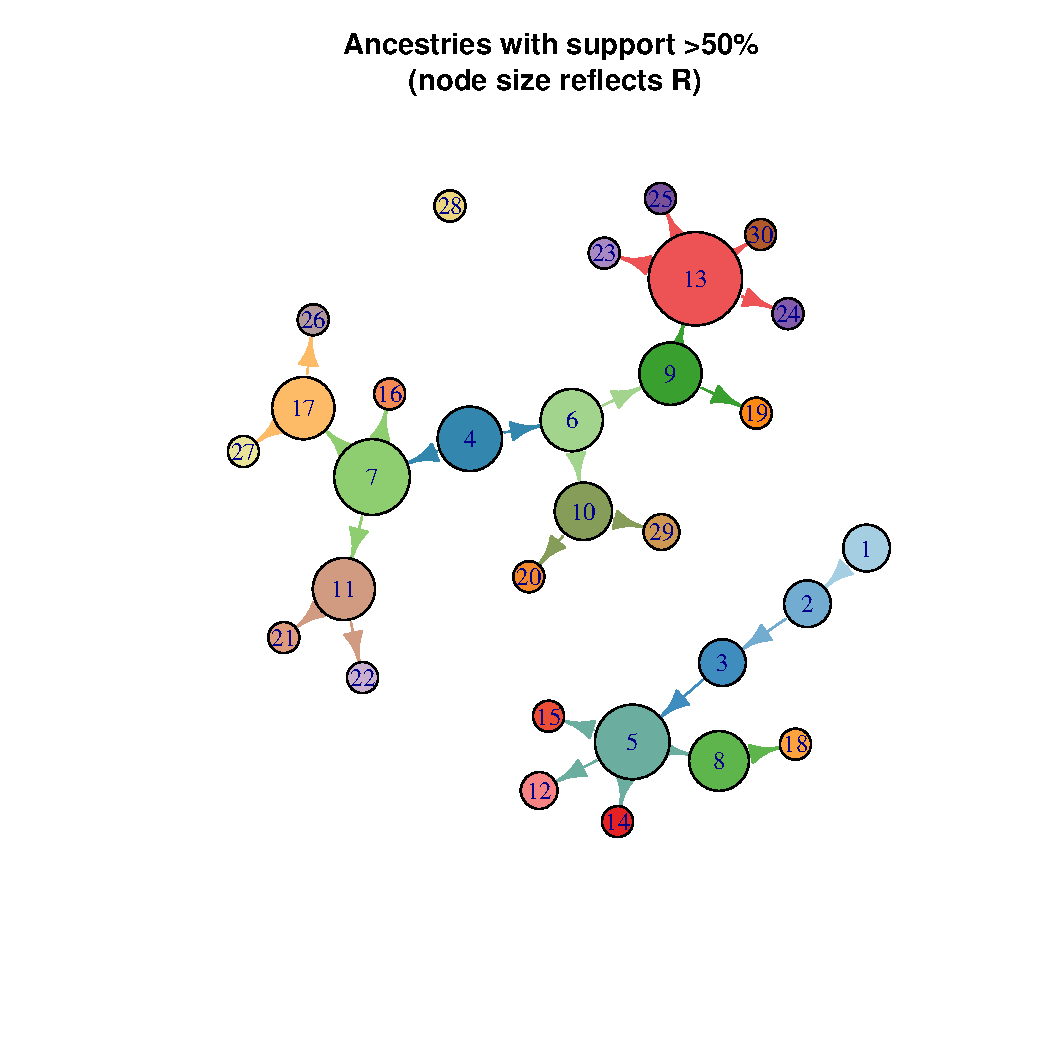
\includegraphics[width=.6\textwidth]{figs/unnamed-chunk-23} 

}



\end{knitrout}

Same idea, but this time colors represent dates of infection:
\begin{knitrout}
\definecolor{shadecolor}{rgb}{0.969, 0.969, 0.969}\color{fgcolor}\begin{kframe}
\begin{alltt}
\hlstd{Tinf} \hlkwb{<-} \hlstd{x[x}\hlopt{$}\hlstd{step}\hlopt{>=}\hlnum{2e4}\hlstd{,}\hlkwd{grep}\hlstd{(}\hlstr{"Tinf"}\hlstd{,} \hlkwd{names}\hlstd{(x))]}
\hlstd{case.color} \hlkwb{<-} \hlkwd{any2col}\hlstd{(}\hlkwd{apply}\hlstd{(Tinf,}\hlnum{2}\hlstd{,mean),} \hlkwc{col.pal}\hlstd{=spectral)}
\hlkwd{plot}\hlstd{(g,} \hlkwc{layout}\hlstd{=layout.auto,} \hlkwc{edge.curved}\hlstd{=}\hlnum{FALSE}\hlstd{,} \hlkwc{vertex.color}\hlstd{=case.color}\hlopt{$}\hlstd{col,}
     \hlkwc{vertex.size}\hlstd{=case.size)}
\hlkwd{title}\hlstd{(}\hlstr{"Ancestries with support >50% \textbackslash{}n(node size reflects R)"}\hlstd{)}
\hlkwd{legend}\hlstd{(}\hlstr{"bottomleft"}\hlstd{,} \hlkwc{col}\hlstd{=case.color}\hlopt{$}\hlstd{leg.col,} \hlkwc{leg}\hlstd{=case.color}\hlopt{$}\hlstd{leg.txt,}
       \hlkwc{title}\hlstd{=}\hlstr{"Mean infection date"}\hlstd{,} \hlkwc{pch}\hlstd{=}\hlnum{20}\hlstd{,} \hlkwc{pt.cex}\hlstd{=}\hlnum{3}\hlstd{,} \hlkwc{inset}\hlstd{=}\hlopt{-}\hlnum{.1}\hlstd{)}
\end{alltt}
\end{kframe}

{\centering 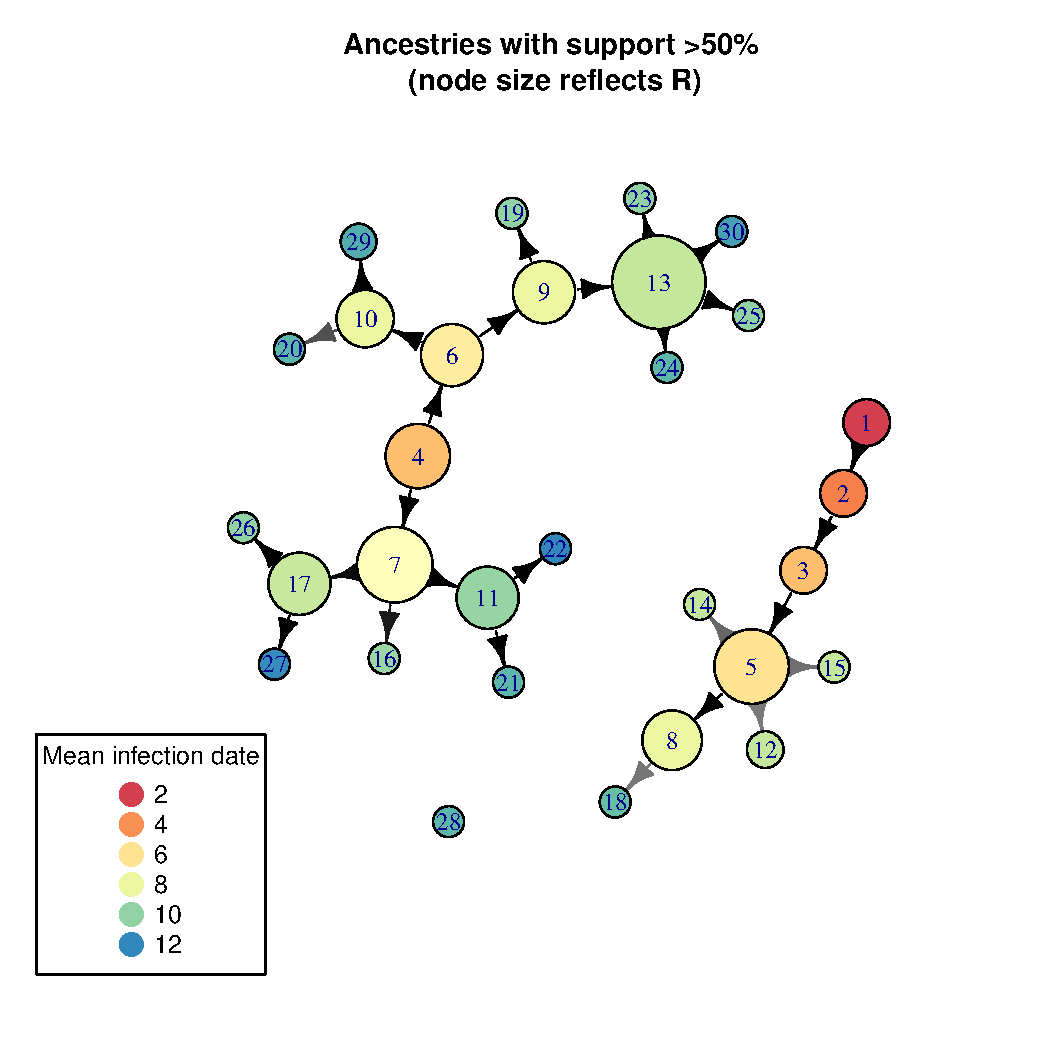
\includegraphics[width=.6\textwidth]{figs/unnamed-chunk-24} 

}



\end{knitrout}


The same can be done with a tree formed by consensus ancestries, obtained by \texttt{get.tTree}:
\begin{knitrout}
\definecolor{shadecolor}{rgb}{0.969, 0.969, 0.969}\color{fgcolor}\begin{kframe}
\begin{alltt}
\hlkwd{plot}\hlstd{(}\hlkwd{get.tTree}\hlstd{(res),} \hlkwc{main}\hlstd{=}\hlstr{"Consensus ancestries - basic plot"}\hlstd{)}
\end{alltt}
\end{kframe}

{\centering 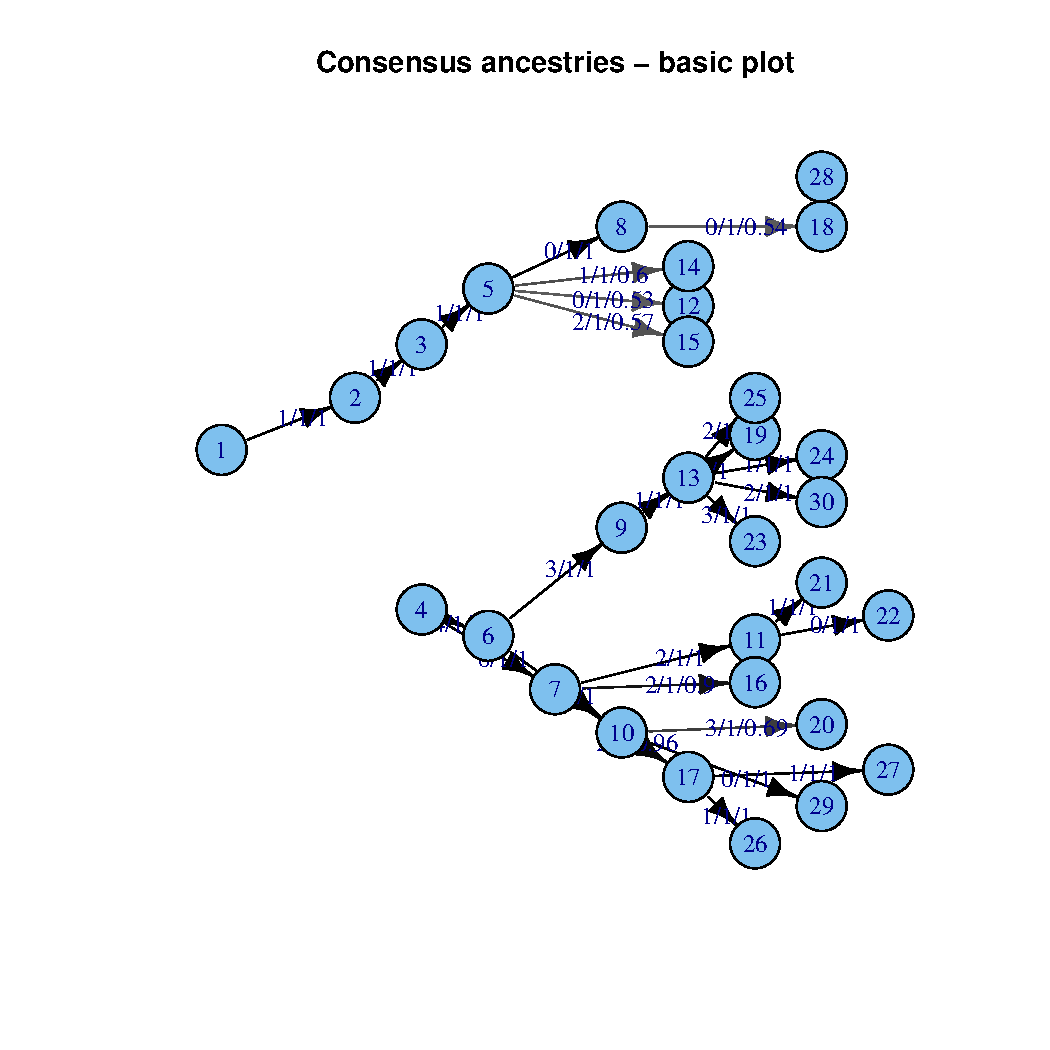
\includegraphics[width=.6\textwidth]{figs/unnamed-chunk-25} 

}



\end{knitrout}


For a customized version where colors represent the mean infection dates:
\begin{knitrout}
\definecolor{shadecolor}{rgb}{0.969, 0.969, 0.969}\color{fgcolor}\begin{kframe}
\begin{alltt}
\hlstd{tre} \hlkwb{<-} \hlkwd{get.tTree}\hlstd{(res)}
\hlkwd{plot}\hlstd{(tre,} \hlkwc{edge.curved}\hlstd{=}\hlnum{TRUE}\hlstd{,} \hlkwc{vertex.color}\hlstd{=case.color}\hlopt{$}\hlstd{col,}
     \hlkwc{vertex.size}\hlstd{=case.size)}
\hlkwd{title}\hlstd{(}\hlstr{"Consensus ancestries \textbackslash{}n(x-axis represents time)"}\hlstd{)}
\hlkwd{legend}\hlstd{(}\hlstr{"bottomleft"}\hlstd{,} \hlkwc{col}\hlstd{=case.color}\hlopt{$}\hlstd{leg.col,} \hlkwc{leg}\hlstd{=case.color}\hlopt{$}\hlstd{leg.txt,}
       \hlkwc{title}\hlstd{=}\hlstr{"Mean infection date"}\hlstd{,} \hlkwc{pch}\hlstd{=}\hlnum{20}\hlstd{,} \hlkwc{pt.cex}\hlstd{=}\hlnum{3}\hlstd{,} \hlkwc{inset}\hlstd{=}\hlopt{-}\hlnum{.1}\hlstd{)}
\end{alltt}
\end{kframe}

{\centering 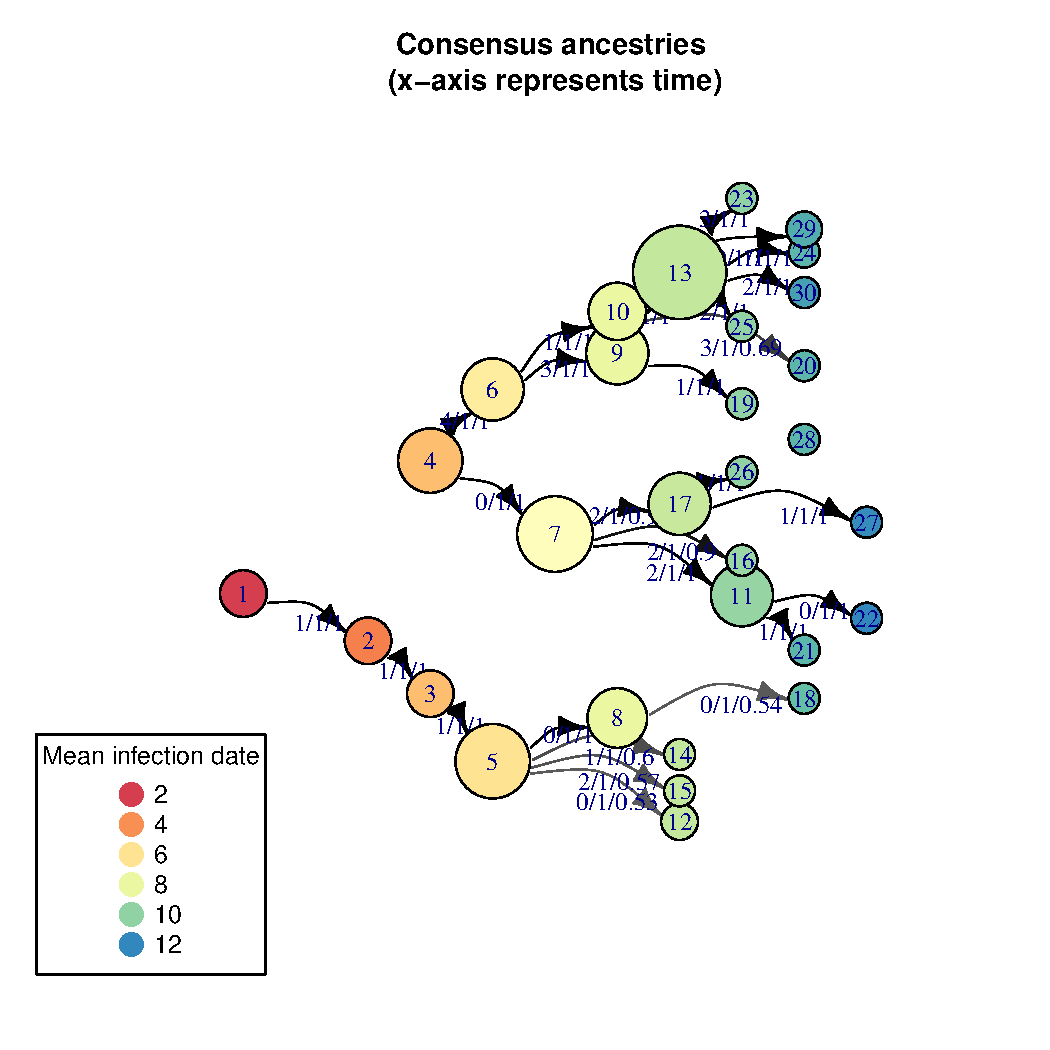
\includegraphics[width=.6\textwidth]{figs/unnamed-chunk-26} 

}



\end{knitrout}

and another, without the time axis:
\begin{knitrout}
\definecolor{shadecolor}{rgb}{0.969, 0.969, 0.969}\color{fgcolor}\begin{kframe}
\begin{alltt}
\hlstd{g} \hlkwb{<-} \hlkwd{as.igraph}\hlstd{(}\hlkwd{get.tTree}\hlstd{(res))}
\hlkwd{plot}\hlstd{(g,} \hlkwc{edge.curved}\hlstd{=}\hlnum{FALSE}\hlstd{,} \hlkwc{vertex.color}\hlstd{=case.color}\hlopt{$}\hlstd{col,} \hlkwc{layout}\hlstd{=layout.auto,}
     \hlkwc{vertex.size}\hlstd{=case.size,} \hlkwc{edge.label}\hlstd{=}\hlstr{""}\hlstd{)}
\hlkwd{title}\hlstd{(}\hlstr{"Consensus ancestries"}\hlstd{)}
\hlkwd{legend}\hlstd{(}\hlstr{"bottomleft"}\hlstd{,} \hlkwc{col}\hlstd{=case.color}\hlopt{$}\hlstd{leg.col,} \hlkwc{leg}\hlstd{=case.color}\hlopt{$}\hlstd{leg.txt,}
       \hlkwc{title}\hlstd{=}\hlstr{"Mean infection date"}\hlstd{,} \hlkwc{pch}\hlstd{=}\hlnum{20}\hlstd{,} \hlkwc{pt.cex}\hlstd{=}\hlnum{3}\hlstd{,} \hlkwc{inset}\hlstd{=}\hlopt{-}\hlnum{.1}\hlstd{)}
\end{alltt}
\end{kframe}

{\centering 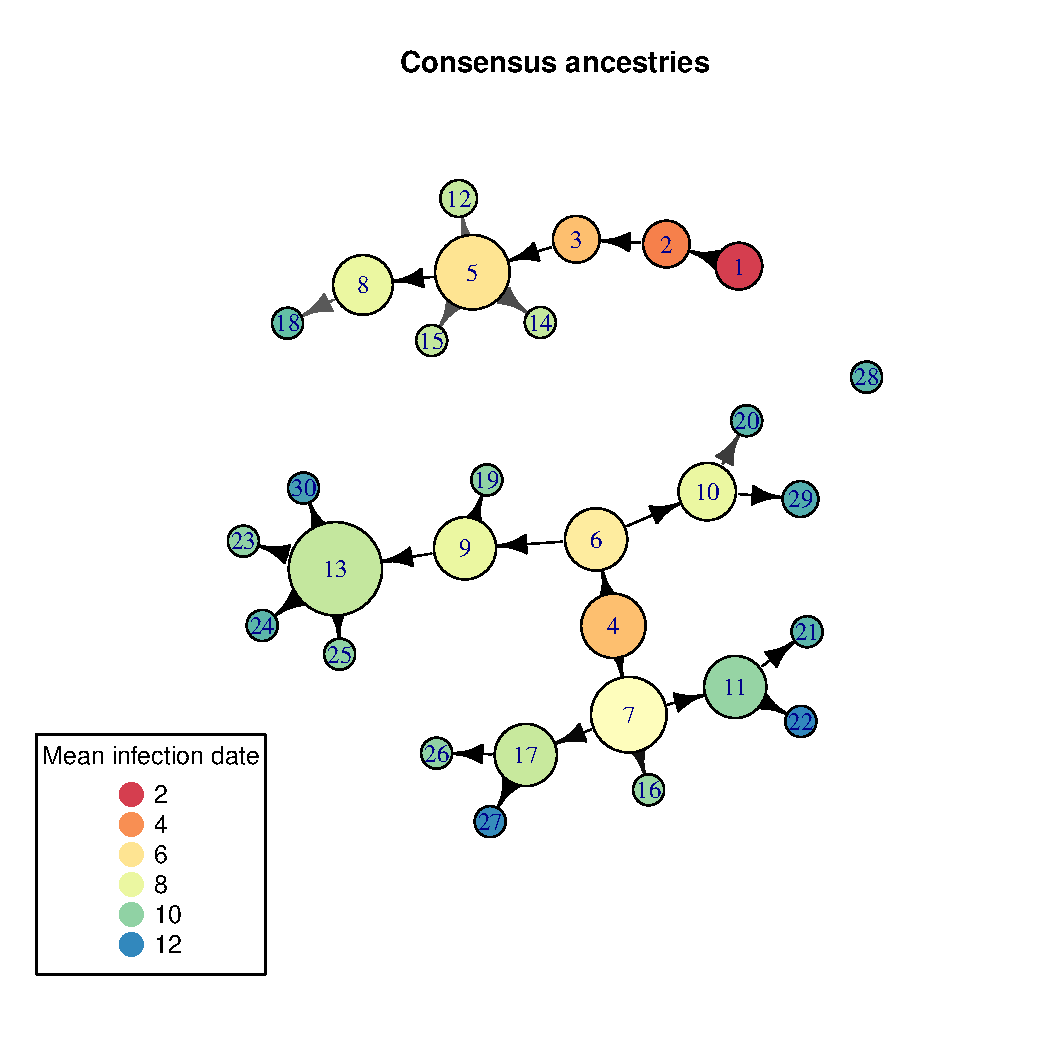
\includegraphics[width=.6\textwidth]{figs/unnamed-chunk-27} 

}



\end{knitrout}

Note that all these plots can be visualized interactively using \texttt{tkplot} (just replace
\texttt{plot} with \texttt{tkplot} in the above command lines).
In all these graphs, we can see that cases 1, 4 and 28 have been classified as imported cases.
For a more systematic assessment of imported cases, we can just look for cases for which the
ancestor is unknown (NA) in the consensus tree:
\begin{knitrout}
\definecolor{shadecolor}{rgb}{0.969, 0.969, 0.969}\color{fgcolor}\begin{kframe}
\begin{alltt}
\hlstd{temp} \hlkwb{<-} \hlkwd{get.tTree}\hlstd{(res)}
\hlstd{temp}\hlopt{$}\hlstd{ances}
\end{alltt}
\begin{verbatim}
##  [1] NA  1  2 NA  3  4  4  5  6  6  7  5  9  5  5  7  7  8  9 10 11 11 13 13 13
## [26] 17 17 NA 10 13
\end{verbatim}
\begin{alltt}
\hlkwd{which}\hlstd{(}\hlkwd{is.na}\hlstd{(temp}\hlopt{$}\hlstd{ances))}
\end{alltt}
\begin{verbatim}
## [1]  1  4 28
\end{verbatim}
\end{kframe}
\end{knitrout}





%%%%%%%%%%%%%%%%%%%%%%%%%%%%%%%%%%%%%%%%%%%%%%%%%%%%
\subsection{Plotting dates of infection}
%%%%%%%%%%%%%%%%%%%%%%%%%%%%%%%%%%%%%%%%%%%%%%%%%%%%

Dates of infection are stored in the table of MCMC outputs, with columns starting with \texttt{Tinf}:
\begin{knitrout}
\definecolor{shadecolor}{rgb}{0.969, 0.969, 0.969}\color{fgcolor}\begin{kframe}
\begin{alltt}
\hlstd{Tinf} \hlkwb{<-} \hlstd{x[x}\hlopt{$}\hlstd{step}\hlopt{>=}\hlnum{2e4}\hlstd{,}\hlkwd{c}\hlstd{(}\hlnum{1}\hlstd{,}\hlkwd{ncol}\hlstd{(x),}\hlkwd{grep}\hlstd{(}\hlstr{"Tinf"}\hlstd{,} \hlkwd{names}\hlstd{(x)))]}
\hlstd{Tinf[}\hlnum{1}\hlopt{:}\hlnum{5}\hlstd{,}\hlnum{1}\hlopt{:}\hlnum{6}\hlstd{]}
\end{alltt}
\begin{verbatim}
##     step run Tinf_1 Tinf_2 Tinf_3 Tinf_4
## 41 20000   1      2      4      5      5
## 42 20500   1      2      4      5      5
## 43 21000   1      2      4      5      5
## 44 21500   1      2      4      5      5
## 45 22000   1      2      3      5      5
\end{verbatim}
\end{kframe}
\end{knitrout}

This information can be visualized easily using the basic \texttt{boxplot}:
\begin{knitrout}
\definecolor{shadecolor}{rgb}{0.969, 0.969, 0.969}\color{fgcolor}\begin{kframe}
\begin{alltt}
\hlkwd{boxplot}\hlstd{(Tinf[,}\hlopt{-}\hlkwd{c}\hlstd{(}\hlnum{1}\hlstd{,}\hlnum{2}\hlstd{)],} \hlkwc{horizontal}\hlstd{=}\hlnum{TRUE}\hlstd{,} \hlkwc{las}\hlstd{=}\hlnum{1}\hlstd{,} \hlkwc{xlab}\hlstd{=}\hlstr{"Date"}\hlstd{,}
        \hlkwc{main}\hlstd{=}\hlstr{"Distribution of infection dates"}\hlstd{,} \hlkwc{col}\hlstd{=}\hlkwd{funky}\hlstd{(}\hlnum{30}\hlstd{))}
\end{alltt}
\end{kframe}

{\centering 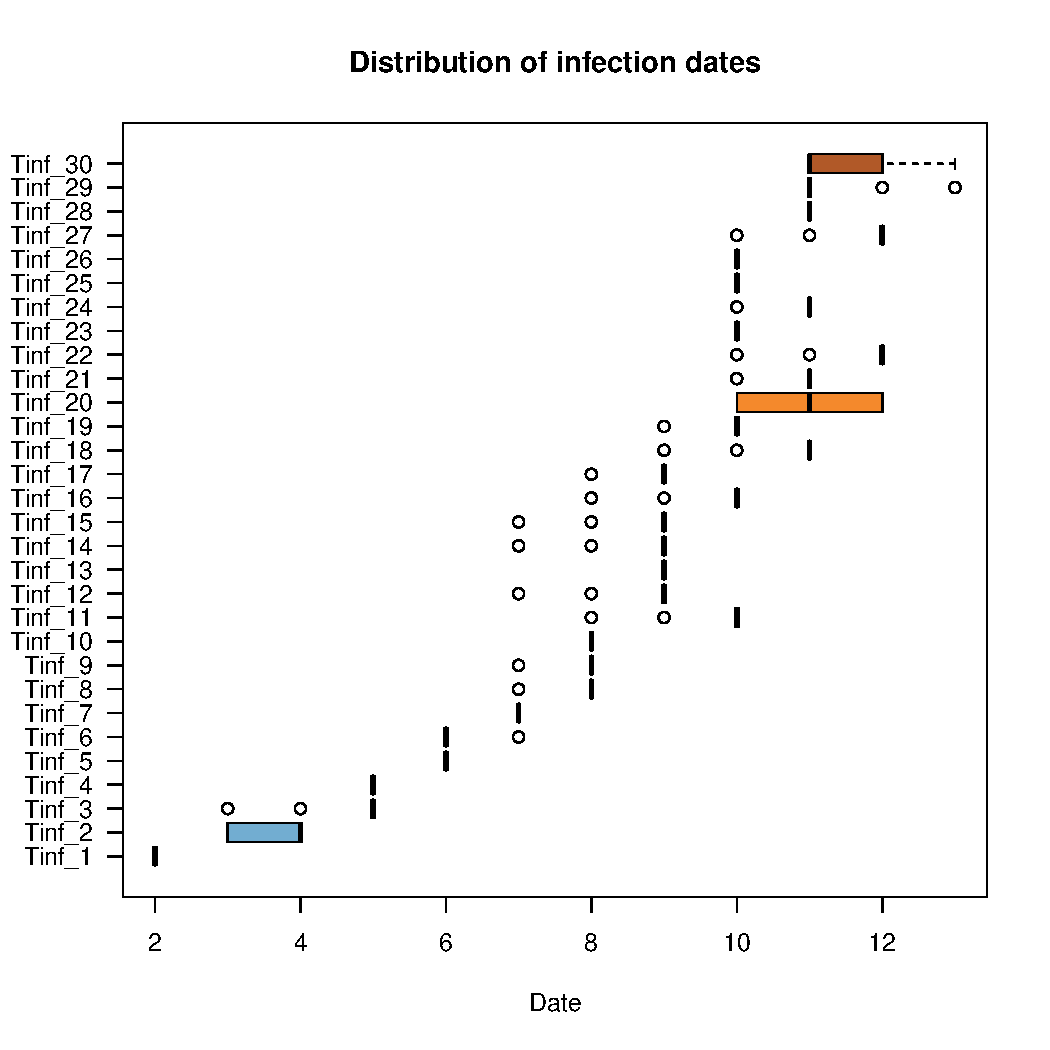
\includegraphics[width=.6\textwidth]{figs/unnamed-chunk-30} 

}



\end{knitrout}

We can also use \textit{ggplot2}, but this demands a slight reformating of the data:
\begin{knitrout}
\definecolor{shadecolor}{rgb}{0.969, 0.969, 0.969}\color{fgcolor}\begin{kframe}
\begin{alltt}
\hlstd{Tinf} \hlkwb{<-} \hlkwd{melt}\hlstd{(Tinf,} \hlkwc{id}\hlstd{=}\hlnum{1}\hlopt{:}\hlnum{2}\hlstd{)}
\hlkwd{names}\hlstd{(Tinf)[}\hlnum{3}\hlopt{:}\hlnum{4}\hlstd{]} \hlkwb{<-} \hlkwd{c}\hlstd{(}\hlstr{"case"}\hlstd{,} \hlstr{"date"}\hlstd{)}
\hlstd{Tinf}\hlopt{$}\hlstd{case} \hlkwb{<-} \hlkwd{sub}\hlstd{(}\hlstr{"Tinf_"}\hlstd{,}\hlstr{"Case "}\hlstd{, Tinf}\hlopt{$}\hlstd{case)}
\hlstd{Tinf}\hlopt{$}\hlstd{case} \hlkwb{<-} \hlkwd{factor}\hlstd{(Tinf}\hlopt{$}\hlstd{case,} \hlkwc{levels}\hlstd{=}\hlkwd{paste}\hlstd{(}\hlstr{"Case"}\hlstd{,}\hlnum{1}\hlopt{:}\hlnum{30}\hlstd{))}
\hlkwd{head}\hlstd{(Tinf)}
\end{alltt}
\begin{verbatim}
##    step run   case date
## 1 20000   1 Case 1    2
## 2 20500   1 Case 1    2
## 3 21000   1 Case 1    2
## 4 21500   1 Case 1    2
## 5 22000   1 Case 1    2
## 6 22500   1 Case 1    2
\end{verbatim}
\begin{alltt}
\hlkwd{tail}\hlstd{(Tinf)}
\end{alltt}
\begin{verbatim}
##         step run    case date
## 19315  97500   4 Case 30   11
## 19316  98000   4 Case 30   12
## 19317  98500   4 Case 30   12
## 19318  99000   4 Case 30   12
## 19319  99500   4 Case 30   12
## 19320 100000   4 Case 30   11
\end{verbatim}
\end{kframe}
\end{knitrout}


In this case, little is gained in the new plot:
\begin{knitrout}
\definecolor{shadecolor}{rgb}{0.969, 0.969, 0.969}\color{fgcolor}\begin{kframe}
\begin{alltt}
\hlstd{p} \hlkwb{<-} \hlkwd{ggplot}\hlstd{(}\hlkwc{data}\hlstd{=Tinf)} \hlopt{+} \hlkwd{geom_boxplot}\hlstd{(}\hlkwd{aes}\hlstd{(}\hlkwc{x}\hlstd{=case,}\hlkwc{y}\hlstd{=date,}\hlkwc{fill}\hlstd{=case),} \hlkwc{alpha}\hlstd{=}\hlnum{.5}\hlstd{)} \hlopt{+}
   \hlkwd{coord_flip}\hlstd{()} \hlopt{+} \hlkwd{labs}\hlstd{(}\hlkwc{y}\hlstd{=}\hlstr{"Infection date"}\hlstd{,} \hlkwc{x}\hlstd{=}\hlstr{""}\hlstd{,} \hlkwc{title}\hlstd{=}\hlstr{"Distribution of infection dates"}\hlstd{)}
\hlstd{p} \hlopt{+} \hlkwd{guides}\hlstd{(}\hlkwc{fill}\hlstd{=}\hlnum{FALSE}\hlstd{)}
\end{alltt}
\end{kframe}

{\centering 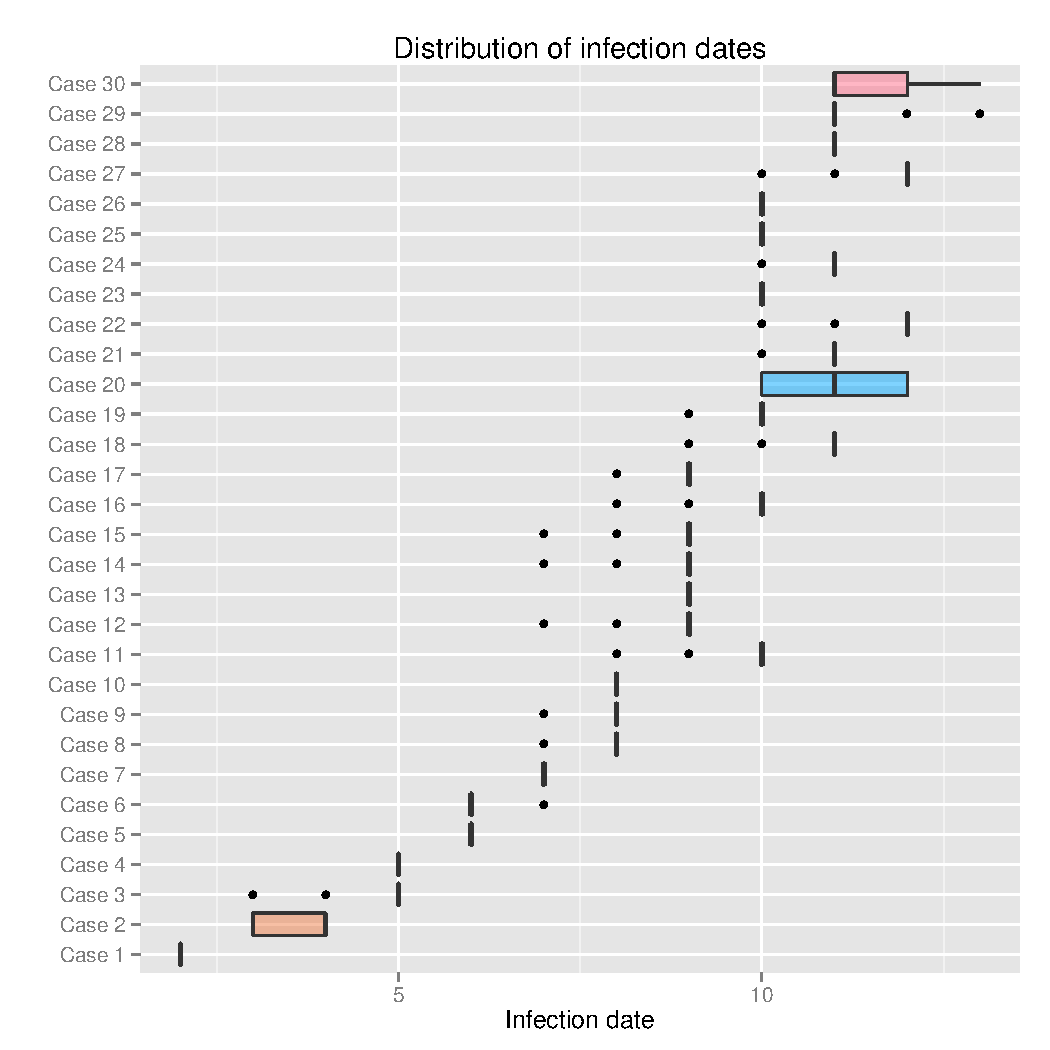
\includegraphics[width=.6\textwidth]{figs/unnamed-chunk-32} 

}



\end{knitrout}


However, it would be simple to compare infection dates of different runs, which may be useful if
different runs provide slightly different results:
\begin{knitrout}
\definecolor{shadecolor}{rgb}{0.969, 0.969, 0.969}\color{fgcolor}\begin{kframe}
\begin{alltt}
\hlkwd{ggplot}\hlstd{(}\hlkwc{data}\hlstd{=Tinf)} \hlopt{+} \hlkwd{geom_boxplot}\hlstd{(}\hlkwd{aes}\hlstd{(}\hlkwc{x}\hlstd{=case,}\hlkwc{y}\hlstd{=date,}\hlkwc{fill}\hlstd{=run),}\hlkwc{alpha}\hlstd{=}\hlnum{.5}\hlstd{)} \hlopt{+} \hlkwd{coord_flip}\hlstd{()} \hlopt{+}
    \hlkwd{labs}\hlstd{(}\hlkwc{y}\hlstd{=}\hlstr{"Infection date"}\hlstd{,} \hlkwc{x}\hlstd{=}\hlstr{""}\hlstd{,} \hlkwc{title}\hlstd{=}\hlstr{"Distribution of infection dates"}\hlstd{)}
\end{alltt}
\end{kframe}

{\centering 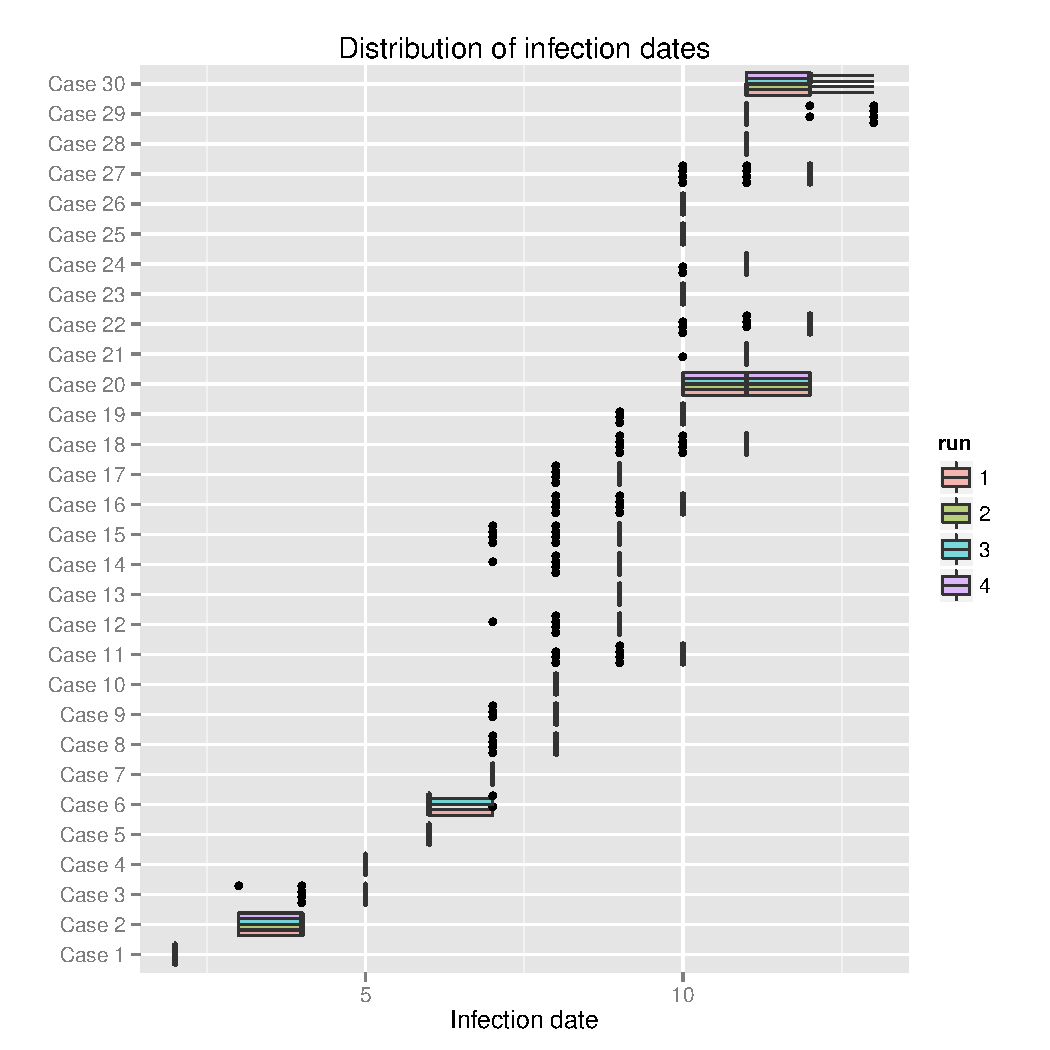
\includegraphics[width=.6\textwidth]{figs/unnamed-chunk-33} 

}



\end{knitrout}





%%%%%%%%%%%%%%%%%%%%%%%%%%%%%%%%%%%%%%%%%%%%%%%%%%%%
\subsection{Accessing posterior distributions}
%%%%%%%%%%%%%%%%%%%%%%%%%%%%%%%%%%%%%%%%%%%%%%%%%%%%

Any element of the model in \texttt{res\$chains} can be plotted using \texttt{plotChains}: it just
needs to be named in the argument \texttt{what}.
For instance, the mutation rate:
\begin{knitrout}
\definecolor{shadecolor}{rgb}{0.969, 0.969, 0.969}\color{fgcolor}\begin{kframe}
\begin{alltt}
\hlkwd{plotChains}\hlstd{(res,} \hlkwc{main}\hlstd{=}\hlstr{"Trace of mu \textbackslash{}n(burnin removed)"}\hlstd{,}
           \hlkwc{burnin}\hlstd{=}\hlnum{2e4}\hlstd{,} \hlkwc{what}\hlstd{=}\hlstr{"mu1"}\hlstd{)}
\end{alltt}
\end{kframe}

{\centering 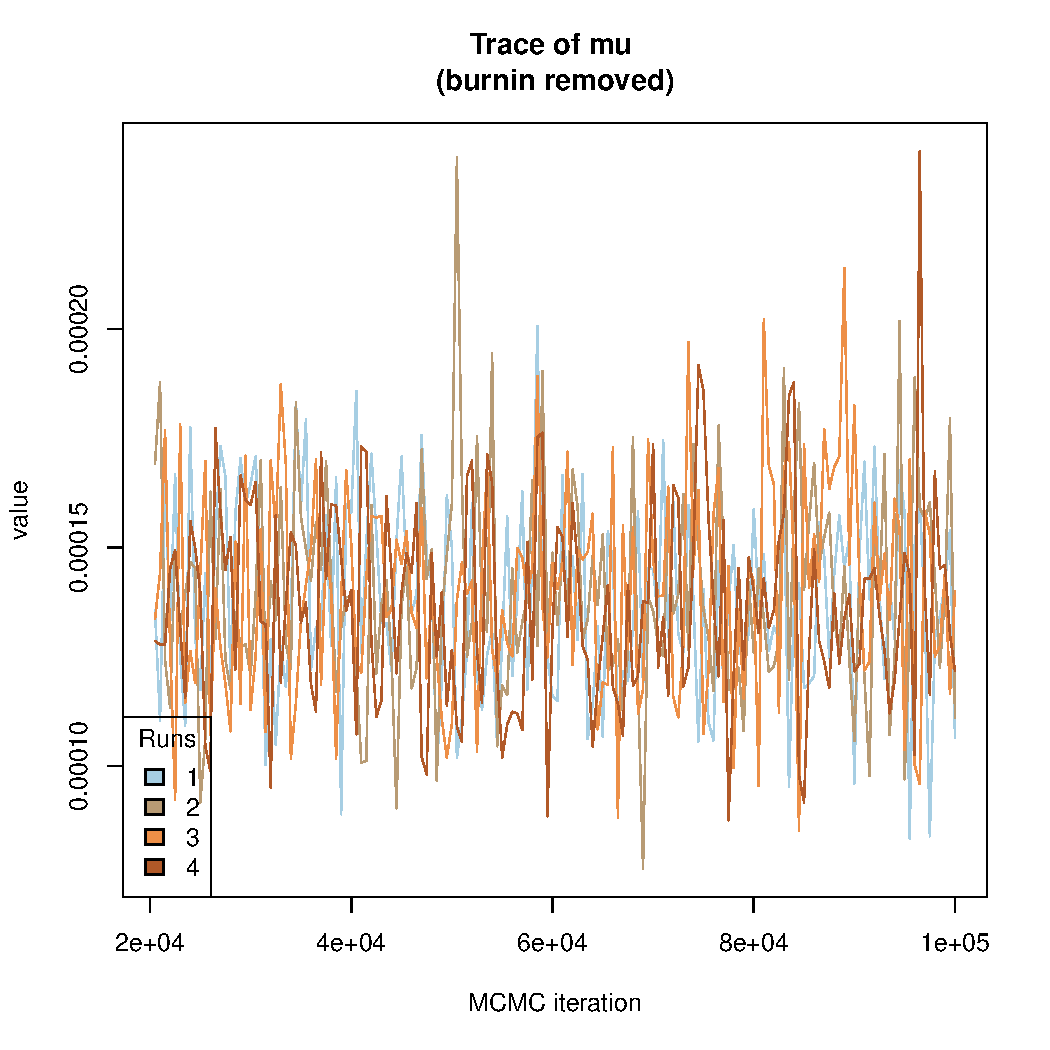
\includegraphics[width=.6\textwidth]{figs/unnamed-chunk-341} 

}


\begin{kframe}\begin{alltt}
\hlkwd{plotChains}\hlstd{(res,} \hlkwc{main}\hlstd{=}\hlstr{"Trace of mu \textbackslash{}n(burnin removed)"}\hlstd{,}
           \hlkwc{burnin}\hlstd{=}\hlnum{2e4}\hlstd{,} \hlkwc{what}\hlstd{=}\hlstr{"mu1"}\hlstd{,} \hlkwc{type}\hlstd{=}\hlstr{"dens"}\hlstd{)}
\end{alltt}
\end{kframe}

{\centering 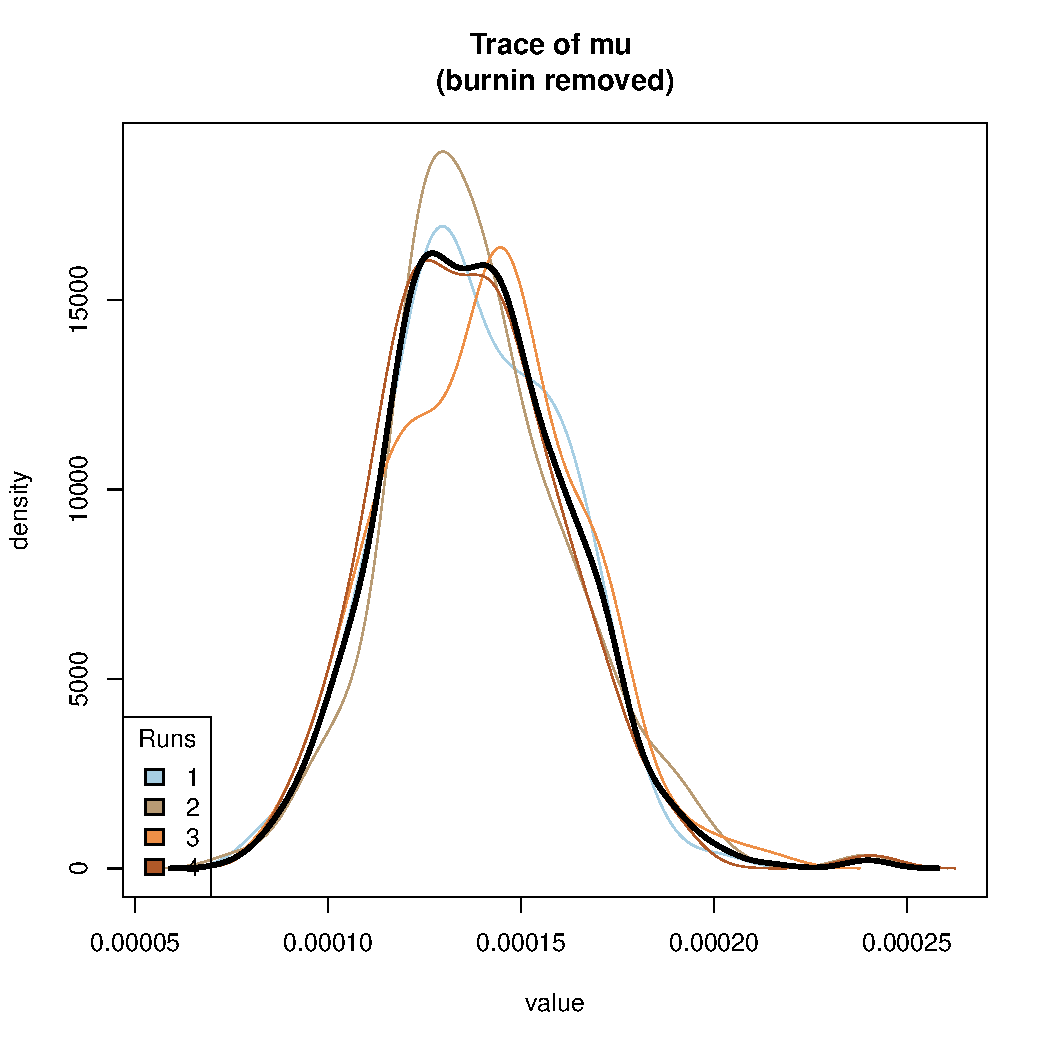
\includegraphics[width=.6\textwidth]{figs/unnamed-chunk-342} 

}



\end{knitrout}

(note that in this case, the plotted information is the mutation rate \textit{per generation of
  infection}, and not per unit of time.
See section on mutation rates below for an estimation of the rates per unit of time.
\\

To derive statistics for a given distribution, one just needs to extract the relevant column, making
sure to remove the burnin:
\begin{knitrout}
\definecolor{shadecolor}{rgb}{0.969, 0.969, 0.969}\color{fgcolor}\begin{kframe}
\begin{alltt}
\hlstd{mu} \hlkwb{<-} \hlstd{res}\hlopt{$}\hlstd{chains}\hlopt{$}\hlstd{mu1[res}\hlopt{$}\hlstd{chains}\hlopt{$}\hlstd{step}\hlopt{>}\hlnum{2e4}\hlstd{]}
\hlkwd{head}\hlstd{(mu)}
\end{alltt}
\begin{verbatim}
## [1] 0.0001356 0.0001104 0.0001644 0.0001324 0.0001667 0.0001252
\end{verbatim}
\begin{alltt}
\hlkwd{length}\hlstd{(mu)}
\end{alltt}
\begin{verbatim}
## [1] 640
\end{verbatim}
\begin{alltt}
\hlkwd{head}\hlstd{(mu)}
\end{alltt}
\begin{verbatim}
## [1] 0.0001356 0.0001104 0.0001644 0.0001324 0.0001667 0.0001252
\end{verbatim}
\begin{alltt}
\hlkwd{summary}\hlstd{(mu)}
\end{alltt}
\begin{verbatim}
##     Min.  1st Qu.   Median     Mean  3rd Qu.     Max. 
## 7.66e-05 1.22e-04 1.38e-04 1.39e-04 1.54e-04 2.41e-04
\end{verbatim}
\end{kframe}
\end{knitrout}

Here we have 640 values to estimate parameters of the distribution of $mu$.
However, the effective sample size might be smaller if successive values are correlated
(autocorrelated chains).
This can be tested easily:
\begin{knitrout}
\definecolor{shadecolor}{rgb}{0.969, 0.969, 0.969}\color{fgcolor}\begin{kframe}
\begin{alltt}
\hlkwd{cor}\hlstd{(mu[}\hlopt{-}\hlkwd{length}\hlstd{(mu)], mu[}\hlnum{2}\hlopt{:}\hlkwd{length}\hlstd{(mu)])}
\end{alltt}
\begin{verbatim}
## [1] 0.02841
\end{verbatim}
\begin{alltt}
\hlkwd{cor.test}\hlstd{(mu[}\hlopt{-}\hlkwd{length}\hlstd{(mu)], mu[}\hlnum{2}\hlopt{:}\hlkwd{length}\hlstd{(mu)])}
\end{alltt}
\begin{verbatim}
## 
## 	Pearson's product-moment correlation
## 
## data:  mu[-length(mu)] and mu[2:length(mu)]
## t = 0.7173, df = 637, p-value = 0.4735
## alternative hypothesis: true correlation is not equal to 0
## 95 percent confidence interval:
##  -0.04926  0.10574
## sample estimates:
##     cor 
## 0.02841
\end{verbatim}
\end{kframe}
\end{knitrout}

No, there is no correlation between successive values.
\\



As before, \texttt{ggplot2} versions of the plot can be obtained; here, for the parameter $\pi$
(proportion of the outbreak sampled):
\begin{knitrout}
\definecolor{shadecolor}{rgb}{0.969, 0.969, 0.969}\color{fgcolor}\begin{kframe}
\begin{alltt}
\hlkwd{library}\hlstd{(ggplot2)}
\hlkwd{library}\hlstd{(reshape2)}
\hlstd{x} \hlkwb{<-} \hlstd{res}\hlopt{$}\hlstd{chains[x}\hlopt{$}\hlstd{step}\hlopt{>}\hlnum{2e4}\hlstd{,]}
\hlstd{x}\hlopt{$}\hlstd{run} \hlkwb{<-} \hlkwd{factor}\hlstd{(x}\hlopt{$}\hlstd{run)}
\end{alltt}
\end{kframe}
\end{knitrout}

To plot densities:
\begin{knitrout}
\definecolor{shadecolor}{rgb}{0.969, 0.969, 0.969}\color{fgcolor}\begin{kframe}
\begin{alltt}
\hlstd{p} \hlkwb{<-} \hlkwd{ggplot}\hlstd{(}\hlkwc{data}\hlstd{=x)} \hlopt{+} \hlkwd{labs}\hlstd{(}\hlkwc{title}\hlstd{=}\hlstr{"Posterior distribution of pi"}\hlstd{,} \hlkwc{x}\hlstd{=}\hlstr{"Pi (proportion of cases sampled)"}\hlstd{)}
\hlstd{p} \hlopt{+} \hlkwd{geom_density}\hlstd{(}\hlkwd{aes}\hlstd{(}\hlkwc{x}\hlstd{=pi,} \hlkwc{fill}\hlstd{=run),} \hlkwc{alpha}\hlstd{=}\hlnum{.3}\hlstd{,} \hlkwc{colour}\hlstd{=}\hlnum{NA}\hlstd{)} \hlopt{+}
    \hlkwd{geom_density}\hlstd{(}\hlkwd{aes}\hlstd{(}\hlkwc{x}\hlstd{=pi),} \hlkwc{size}\hlstd{=}\hlnum{1}\hlstd{,} \hlkwc{colour}\hlstd{=}\hlstr{"black"}\hlstd{,} \hlkwc{shape}\hlstd{=}\hlnum{2}\hlstd{,} \hlkwc{alpha}\hlstd{=}\hlnum{.8}\hlstd{)}
\end{alltt}
\end{kframe}

{\centering 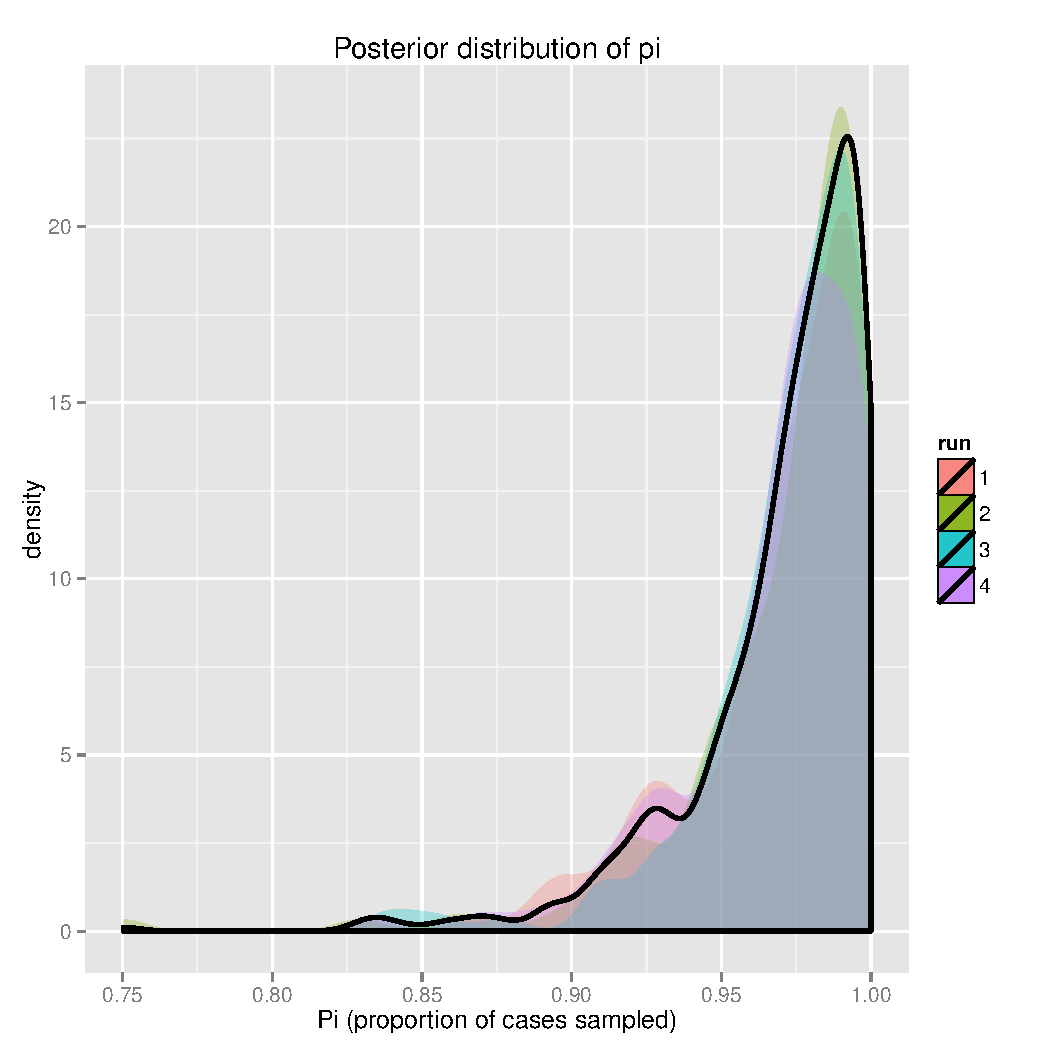
\includegraphics[width=.6\textwidth]{figs/unnamed-chunk-38} 

}



\end{knitrout}

Histograms:
\begin{knitrout}
\definecolor{shadecolor}{rgb}{0.969, 0.969, 0.969}\color{fgcolor}\begin{kframe}
\begin{alltt}
\hlstd{p} \hlopt{+} \hlkwd{geom_histogram}\hlstd{(}\hlkwd{aes}\hlstd{(}\hlkwc{x}\hlstd{=pi,} \hlkwc{fill}\hlstd{=run,} \hlkwc{y}\hlstd{=..density..),} \hlkwc{alpha}\hlstd{=}\hlnum{.7}\hlstd{,} \hlkwc{colour}\hlstd{=}\hlnum{NA}\hlstd{,} \hlkwc{position}\hlstd{=}\hlstr{"dodge"}\hlstd{)} \hlopt{+}
    \hlkwd{geom_density}\hlstd{(}\hlkwd{aes}\hlstd{(}\hlkwc{x}\hlstd{=pi),} \hlkwc{size}\hlstd{=}\hlnum{1}\hlstd{,} \hlkwc{colour}\hlstd{=}\hlstr{"black"}\hlstd{,} \hlkwc{shape}\hlstd{=}\hlnum{2}\hlstd{,} \hlkwc{alpha}\hlstd{=}\hlnum{.8}\hlstd{)}
\end{alltt}


{\ttfamily\noindent\itshape\color{messagecolor}{\#\# stat\_bin: binwidth defaulted to range/30. Use 'binwidth = x' to adjust this.}}\end{kframe}

{\centering 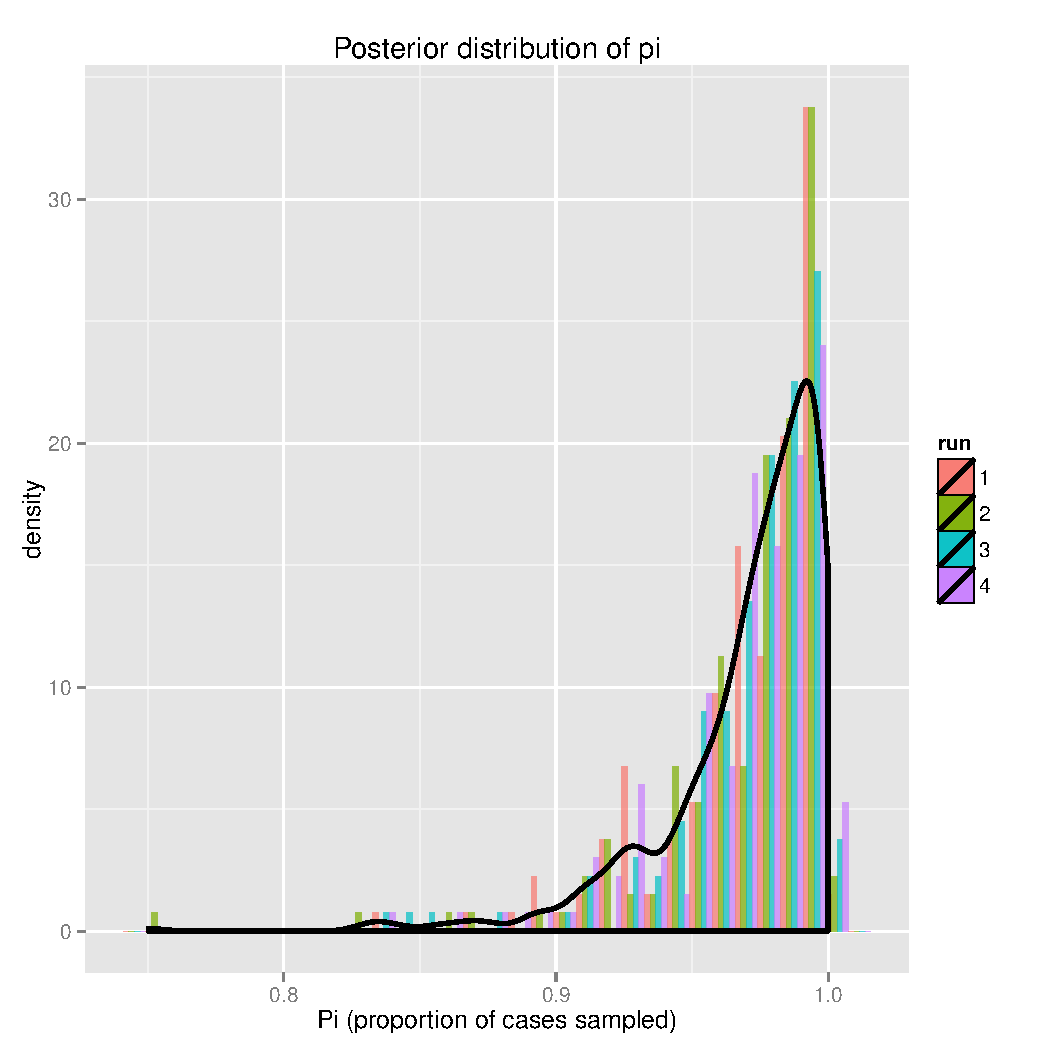
\includegraphics[width=.6\textwidth]{figs/unnamed-chunk-39} 

}



\end{knitrout}

Using different boxplots for different runs:
\begin{knitrout}
\definecolor{shadecolor}{rgb}{0.969, 0.969, 0.969}\color{fgcolor}\begin{kframe}
\begin{alltt}
\hlstd{p} \hlopt{+} \hlkwd{geom_boxplot}\hlstd{(}\hlkwd{aes}\hlstd{(}\hlkwc{x}\hlstd{=run,} \hlkwc{y}\hlstd{=pi,} \hlkwc{fill}\hlstd{=run),}\hlkwc{alpha}\hlstd{=}\hlnum{.6}\hlstd{)} \hlopt{+}
    \hlkwd{geom_jitter}\hlstd{(}\hlkwd{aes}\hlstd{(}\hlkwc{x}\hlstd{=run,} \hlkwc{y}\hlstd{=pi,} \hlkwc{col}\hlstd{=run),}\hlkwc{alpha}\hlstd{=}\hlnum{.4}\hlstd{)}
\end{alltt}
\end{kframe}

{\centering 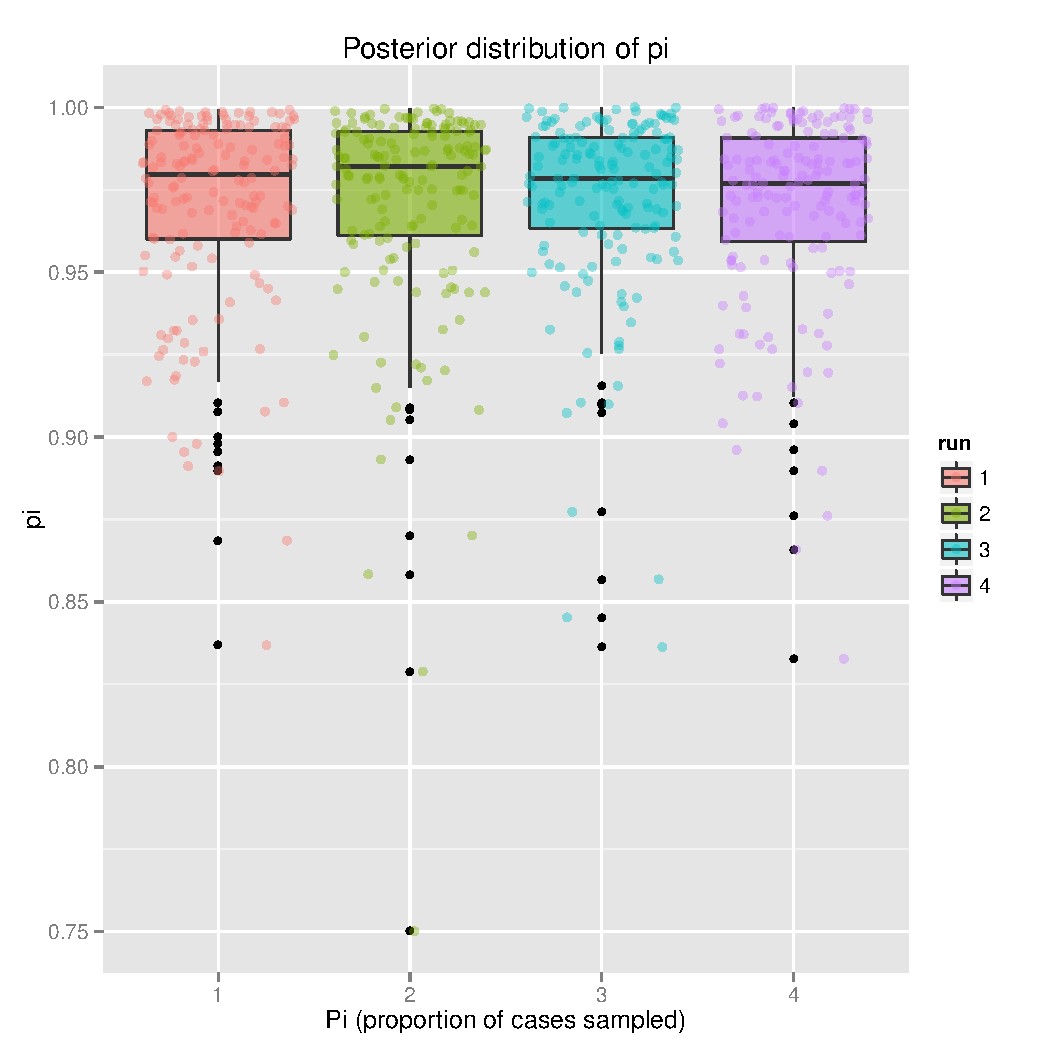
\includegraphics[width=.6\textwidth]{figs/unnamed-chunk-40} 

}



\end{knitrout}

Same idea, but using violinplots:
\begin{knitrout}
\definecolor{shadecolor}{rgb}{0.969, 0.969, 0.969}\color{fgcolor}\begin{kframe}
\begin{alltt}
\hlstd{p} \hlopt{+} \hlkwd{geom_violin}\hlstd{(}\hlkwd{aes}\hlstd{(}\hlkwc{x}\hlstd{=run,} \hlkwc{y}\hlstd{=pi,} \hlkwc{fill}\hlstd{=run),}\hlkwc{alpha}\hlstd{=}\hlnum{.6}\hlstd{)}
\end{alltt}
\end{kframe}

{\centering 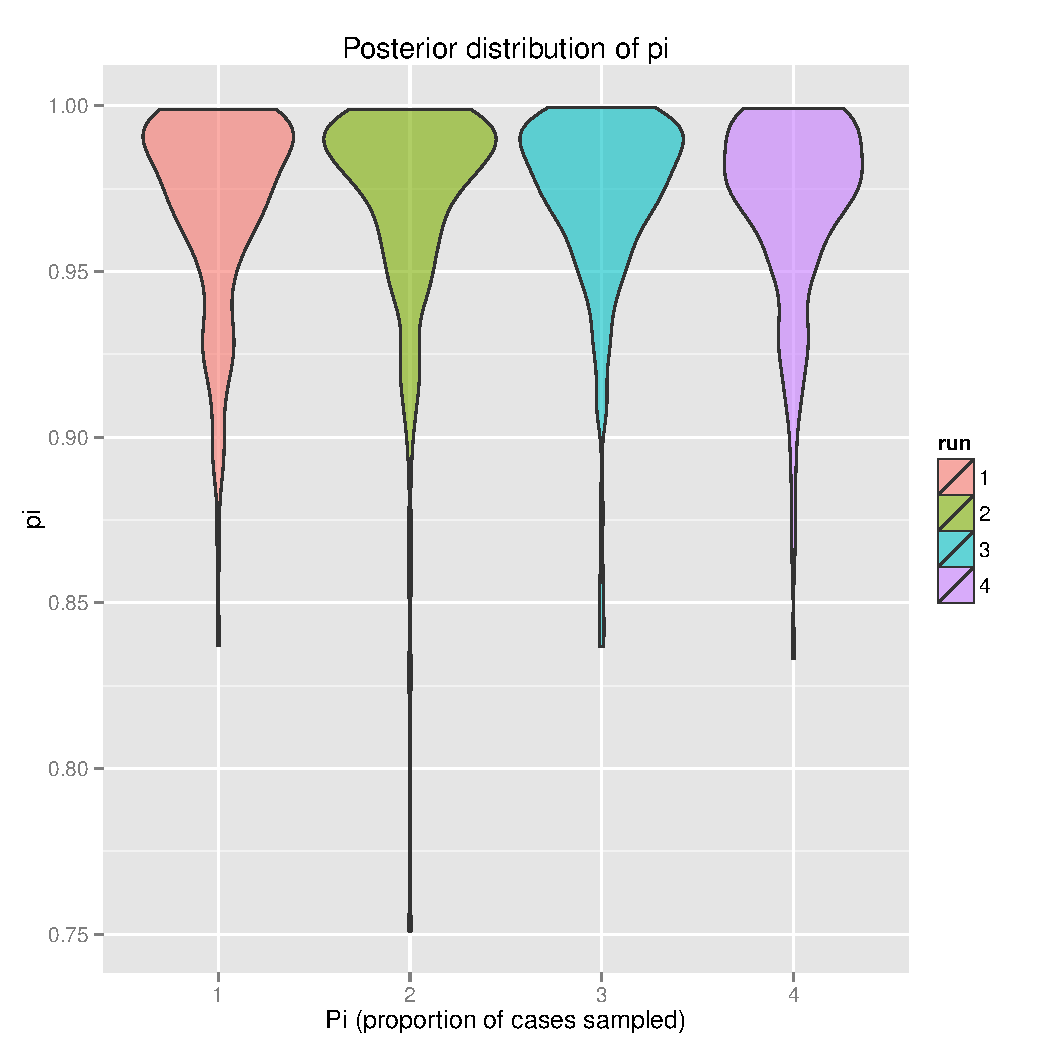
\includegraphics[width=.6\textwidth]{figs/unnamed-chunk-41} 

}



\end{knitrout}






%%%%%%%%%%%%%%%%%%%%%%%%%%%%%%%%%%%%%%%%%%%%%%%%%%%%
\subsection{Mutation rates}
%%%%%%%%%%%%%%%%%%%%%%%%%%%%%%%%%%%%%%%%%%%%%%%%%%%%
As mentioned before, mutation rates in \textit{outbreaker}'s model are expressed per generation of infection.
However, mutation rates per unit of time are biologically easier to interpret.
These can be obtained using \texttt{get.mu}:
\begin{knitrout}
\definecolor{shadecolor}{rgb}{0.969, 0.969, 0.969}\color{fgcolor}\begin{kframe}
\begin{alltt}
\hlstd{mu} \hlkwb{<-} \hlkwd{get.mu}\hlstd{(res,} \hlkwc{burnin}\hlstd{=}\hlnum{2e4}\hlstd{)}
\hlkwd{summary}\hlstd{(mu)}
\end{alltt}
\begin{verbatim}
##    Min. 1st Qu.  Median    Mean 3rd Qu.    Max. 
##   0.827   0.877   0.914   0.914   0.944   1.060
\end{verbatim}
\begin{alltt}
\hlkwd{hist}\hlstd{(mu,} \hlkwc{col}\hlstd{=}\hlstr{"grey"}\hlstd{,}\hlkwc{border}\hlstd{=}\hlstr{"lightgrey"}\hlstd{,} \hlkwc{xlab}\hlstd{=}\hlstr{"Mutation rate (per genome and unit time)"}\hlstd{,}
     \hlkwc{main}\hlstd{=}\hlstr{"Posterior distribution of mu"}\hlstd{)}
\end{alltt}
\end{kframe}

{\centering 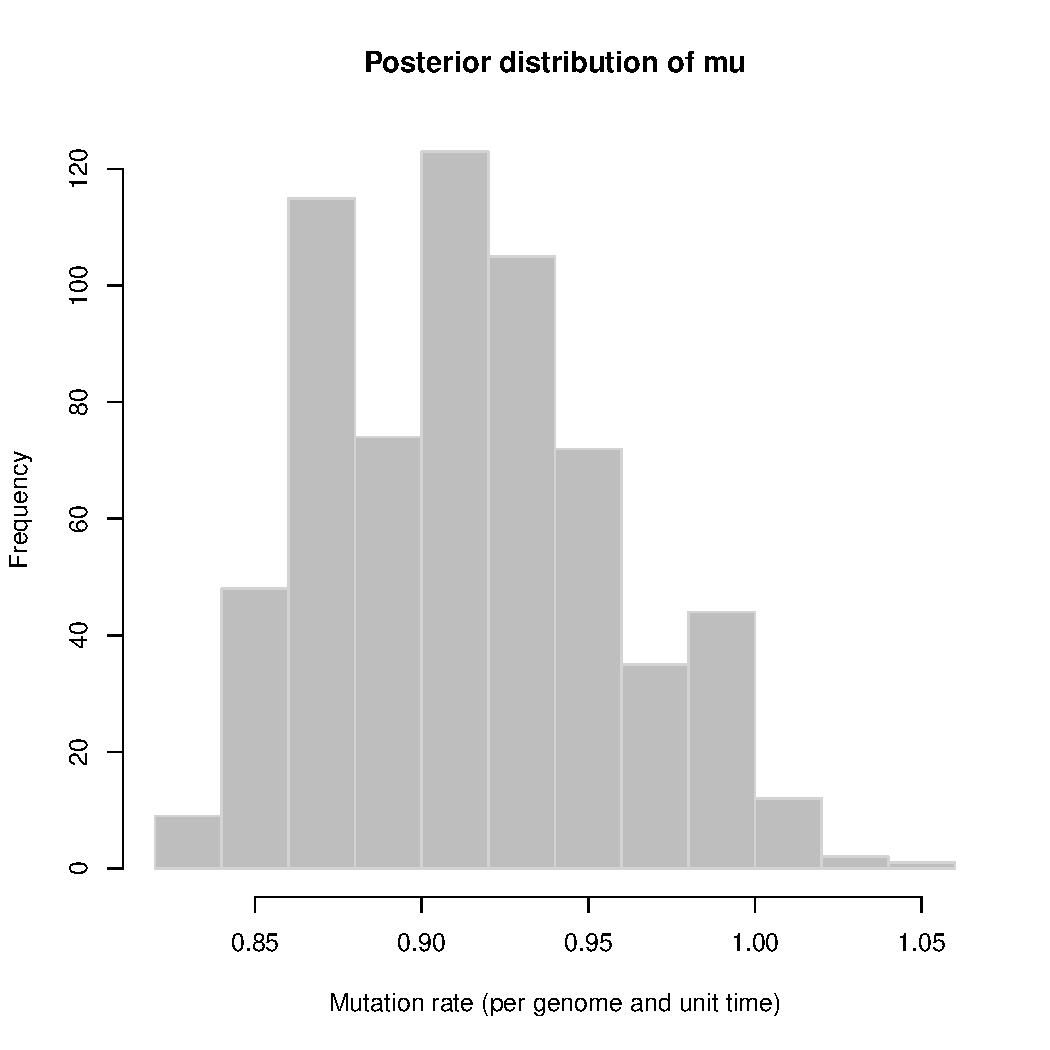
\includegraphics[width=.6\textwidth]{figs/unnamed-chunk-42} 

}



\end{knitrout}


Re-expressing the rates per nucleotide, and adding the media and 95\%credibility interval to the histogram:
\begin{knitrout}
\definecolor{shadecolor}{rgb}{0.969, 0.969, 0.969}\color{fgcolor}\begin{kframe}
\begin{alltt}
\hlstd{mu} \hlkwb{<-} \hlkwd{get.mu}\hlstd{(res,} \hlkwc{burnin}\hlstd{=}\hlnum{2e4}\hlstd{,} \hlkwc{genome.size}\hlstd{=}\hlkwd{ncol}\hlstd{(dat}\hlopt{$}\hlstd{dna))}
\hlkwd{summary}\hlstd{(mu)}
\end{alltt}
\begin{verbatim}
##     Min.  1st Qu.   Median     Mean  3rd Qu.     Max. 
## 8.27e-05 8.77e-05 9.14e-05 9.14e-05 9.44e-05 1.06e-04
\end{verbatim}
\begin{alltt}
\hlkwd{hist}\hlstd{(mu,} \hlkwc{col}\hlstd{=}\hlstr{"grey"}\hlstd{,}\hlkwc{border}\hlstd{=}\hlstr{"lightgrey"}\hlstd{,} \hlkwc{xlab}\hlstd{=}\hlstr{"Mutation rate (per genome and unit time)"}\hlstd{,}
     \hlkwc{main}\hlstd{=}\hlstr{"Posterior distribution of mu"}\hlstd{)}
\hlkwd{abline}\hlstd{(}\hlkwc{v}\hlstd{=}\hlkwd{quantile}\hlstd{(mu,} \hlkwd{c}\hlstd{(}\hlnum{.025}\hlstd{,} \hlnum{.5}\hlstd{,} \hlnum{.975}\hlstd{)),} \hlkwc{lty}\hlstd{=}\hlkwd{c}\hlstd{(}\hlnum{2}\hlstd{,}\hlnum{1}\hlstd{,}\hlnum{2}\hlstd{),} \hlkwc{lwd}\hlstd{=}\hlnum{2}\hlstd{,} \hlkwc{col}\hlstd{=}\hlstr{"royalblue"}\hlstd{)}
\hlkwd{legend}\hlstd{(}\hlstr{"topright"}\hlstd{,} \hlkwc{lty}\hlstd{=}\hlkwd{c}\hlstd{(}\hlnum{1}\hlstd{,}\hlnum{2}\hlstd{),} \hlkwc{leg}\hlstd{=}\hlkwd{c}\hlstd{(}\hlstr{"Median"}\hlstd{,}\hlstr{"95% credibility interval"}\hlstd{),}
       \hlkwc{col}\hlstd{=}\hlstr{"royalblue"}\hlstd{,} \hlkwc{bg}\hlstd{=}\hlstr{"white"}\hlstd{)}
\end{alltt}
\end{kframe}

{\centering 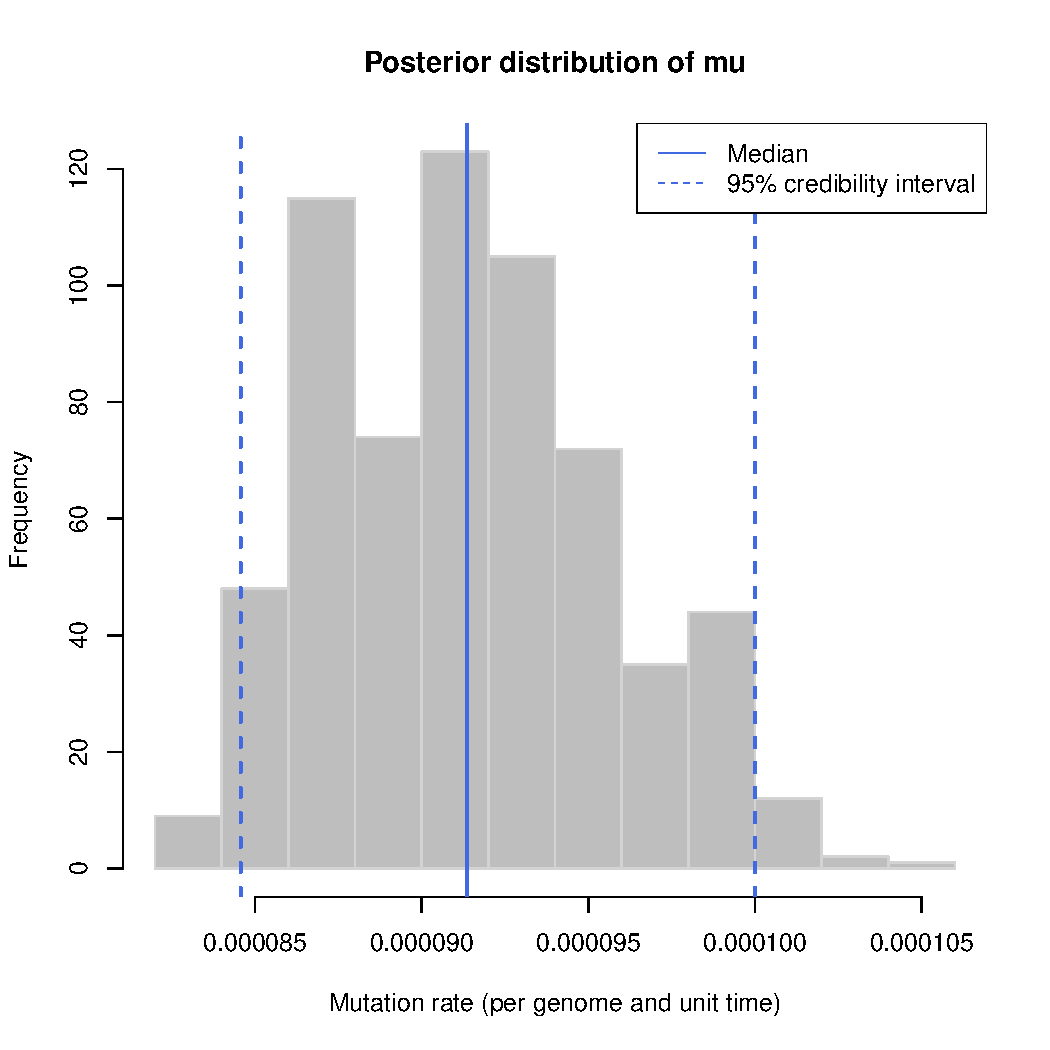
\includegraphics[width=.6\textwidth]{figs/unnamed-chunk-43} 

}



\end{knitrout}


Same idea, using a one-dimensional density estimation:
\begin{knitrout}
\definecolor{shadecolor}{rgb}{0.969, 0.969, 0.969}\color{fgcolor}\begin{kframe}
\begin{alltt}
\hlkwd{plot}\hlstd{(}\hlkwd{density}\hlstd{(mu),} \hlkwc{xlab}\hlstd{=}\hlstr{"Mutation rate (per genome and unit time)"}\hlstd{,}
     \hlkwc{main}\hlstd{=}\hlstr{"Posterior distribution of mu"}\hlstd{,} \hlkwc{lwd}\hlstd{=}\hlnum{3}\hlstd{)}
\hlkwd{points}\hlstd{(}\hlkwd{jitter}\hlstd{(mu),} \hlkwd{rep}\hlstd{(}\hlnum{0}\hlstd{,} \hlkwd{length}\hlstd{(mu)),} \hlkwc{pch}\hlstd{=}\hlstr{"|"}\hlstd{,} \hlkwc{col}\hlstd{=}\hlkwd{transp}\hlstd{(}\hlstr{"blue"}\hlstd{))}
\hlkwd{abline}\hlstd{(}\hlkwc{v}\hlstd{=}\hlkwd{quantile}\hlstd{(mu,} \hlkwd{c}\hlstd{(}\hlnum{.025}\hlstd{,} \hlnum{.5}\hlstd{,} \hlnum{.975}\hlstd{)),} \hlkwc{lty}\hlstd{=}\hlkwd{c}\hlstd{(}\hlnum{2}\hlstd{,}\hlnum{1}\hlstd{,}\hlnum{2}\hlstd{),} \hlkwc{lwd}\hlstd{=}\hlnum{2}\hlstd{,} \hlkwc{col}\hlstd{=}\hlstr{"royalblue"}\hlstd{)}
\hlkwd{legend}\hlstd{(}\hlstr{"topright"}\hlstd{,} \hlkwc{lty}\hlstd{=}\hlkwd{c}\hlstd{(}\hlnum{1}\hlstd{,}\hlnum{2}\hlstd{),} \hlkwc{leg}\hlstd{=}\hlkwd{c}\hlstd{(}\hlstr{"Median"}\hlstd{,}\hlstr{"95% credibility interval"}\hlstd{),}
       \hlkwc{col}\hlstd{=}\hlstr{"royalblue"}\hlstd{,} \hlkwc{bg}\hlstd{=}\hlstr{"white"}\hlstd{)}
\end{alltt}
\end{kframe}

{\centering 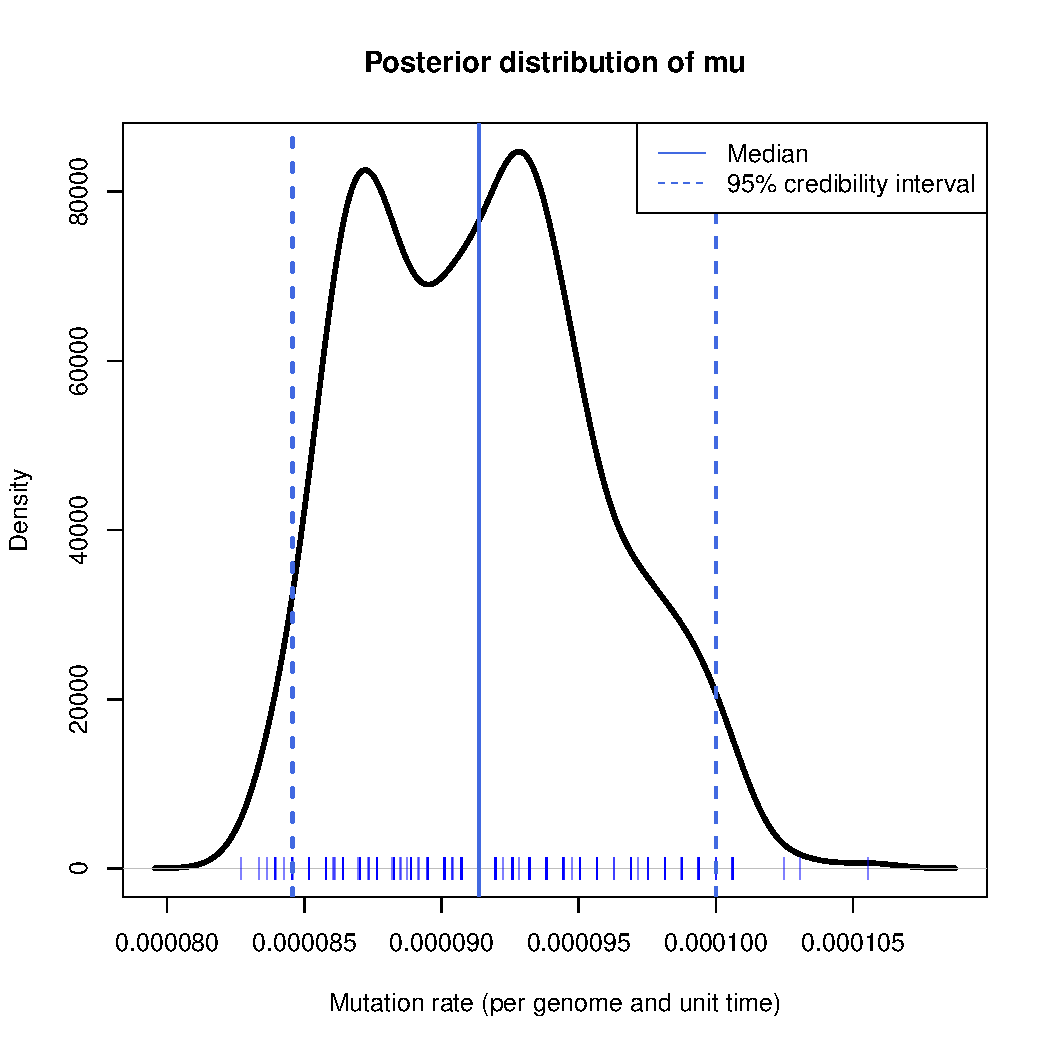
\includegraphics[width=.6\textwidth]{figs/unnamed-chunk-44} 

}



\end{knitrout}






%%%%%%%%%%%%%%%%%%%%%%%%%%%%%%%%%%%%%%%%%%%%%%%%%%%%
\subsection{Incidence and reproduction numbers}
%%%%%%%%%%%%%%%%%%%%%%%%%%%%%%%%%%%%%%%%%%%%%%%%%%%%

Incidence curves and effective reproduction numbers can be derived from the results of \textit{outbreaker}.
Incidence curves can be obtained and visualized using \texttt{get.incid}:
\begin{knitrout}
\definecolor{shadecolor}{rgb}{0.969, 0.969, 0.969}\color{fgcolor}\begin{kframe}
\begin{alltt}
\hlstd{incid} \hlkwb{<-} \hlkwd{get.incid}\hlstd{(res,} \hlkwc{burnin}\hlstd{=}\hlnum{2e4}\hlstd{)}
\end{alltt}
\end{kframe}

{\centering 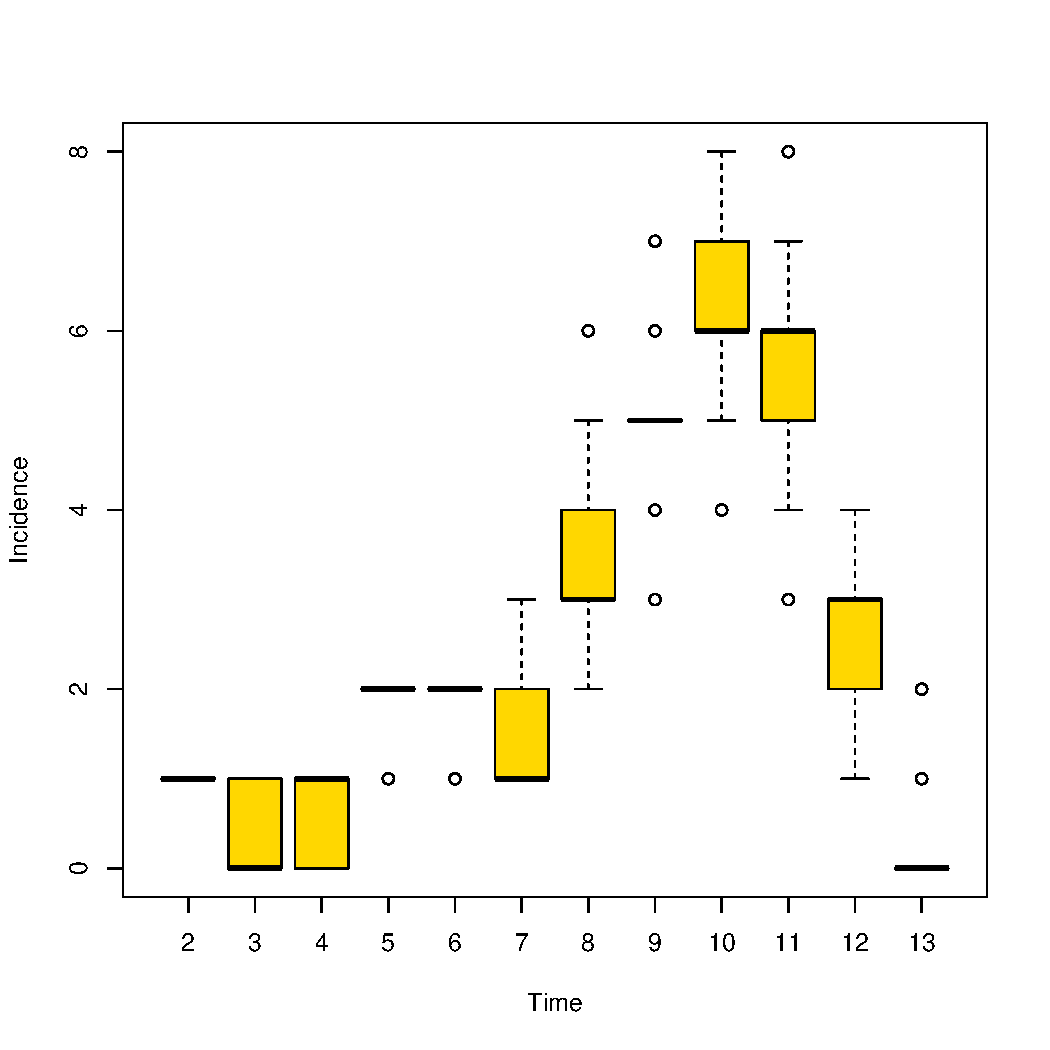
\includegraphics[width=.6\textwidth]{figs/unnamed-chunk-45} 

}


\begin{kframe}\begin{alltt}
\hlkwd{class}\hlstd{(incid)}
\end{alltt}
\begin{verbatim}
## [1] "matrix"
\end{verbatim}
\begin{alltt}
\hlkwd{dim}\hlstd{(incid)}
\end{alltt}
\begin{verbatim}
## [1]  12 640
\end{verbatim}
\begin{alltt}
\hlstd{incid[,}\hlnum{1}\hlopt{:}\hlnum{10}\hlstd{]}
\end{alltt}
\begin{verbatim}
##    init                  
## 2     1 1 1 1 1 1 1 1 1 1
## 3     0 0 0 1 0 0 1 0 0 0
## 4     1 1 1 0 1 1 0 1 1 1
## 5     2 2 2 2 2 2 2 2 2 2
## 6     2 2 2 2 2 2 2 2 2 2
## 7     1 1 1 1 1 1 1 1 1 1
## 8     4 3 3 3 4 4 3 3 4 3
## 9     4 5 6 6 4 4 5 7 4 6
## 10    7 7 5 6 6 6 6 6 6 5
## 11    6 5 6 5 7 7 6 4 7 7
## 12    2 3 3 3 2 2 3 3 2 2
## 13    0 0 0 0 0 0 0 0 0 0
\end{verbatim}
\end{kframe}
\end{knitrout}

Each column in \texttt{incid} is a different realization of an incidence curve corresponding to one
step of the MCMC.
Other graphical options are available:
\begin{knitrout}
\definecolor{shadecolor}{rgb}{0.969, 0.969, 0.969}\color{fgcolor}\begin{kframe}
\begin{alltt}
\hlkwd{args}\hlstd{(get.incid)}
\end{alltt}
\begin{verbatim}
## function (x, burnin = 20000, plot = TRUE, type = c("boxplot", 
##     "lines"), lines = FALSE, fill.col = "gold", lines.col = transp("grey"), 
##     ...) 
## NULL
\end{verbatim}
\begin{alltt}
\hlstd{incid} \hlkwb{<-} \hlkwd{get.incid}\hlstd{(res,} \hlkwc{type}\hlstd{=}\hlstr{"lines"}\hlstd{,}\hlkwc{lines.col}\hlstd{=}\hlkwd{transp}\hlstd{(}\hlstr{"black"}\hlstd{,}\hlnum{.1}\hlstd{))}
\hlkwd{title}\hlstd{(}\hlstr{"Posterior estimates of incidence"}\hlstd{)}
\end{alltt}
\end{kframe}

{\centering 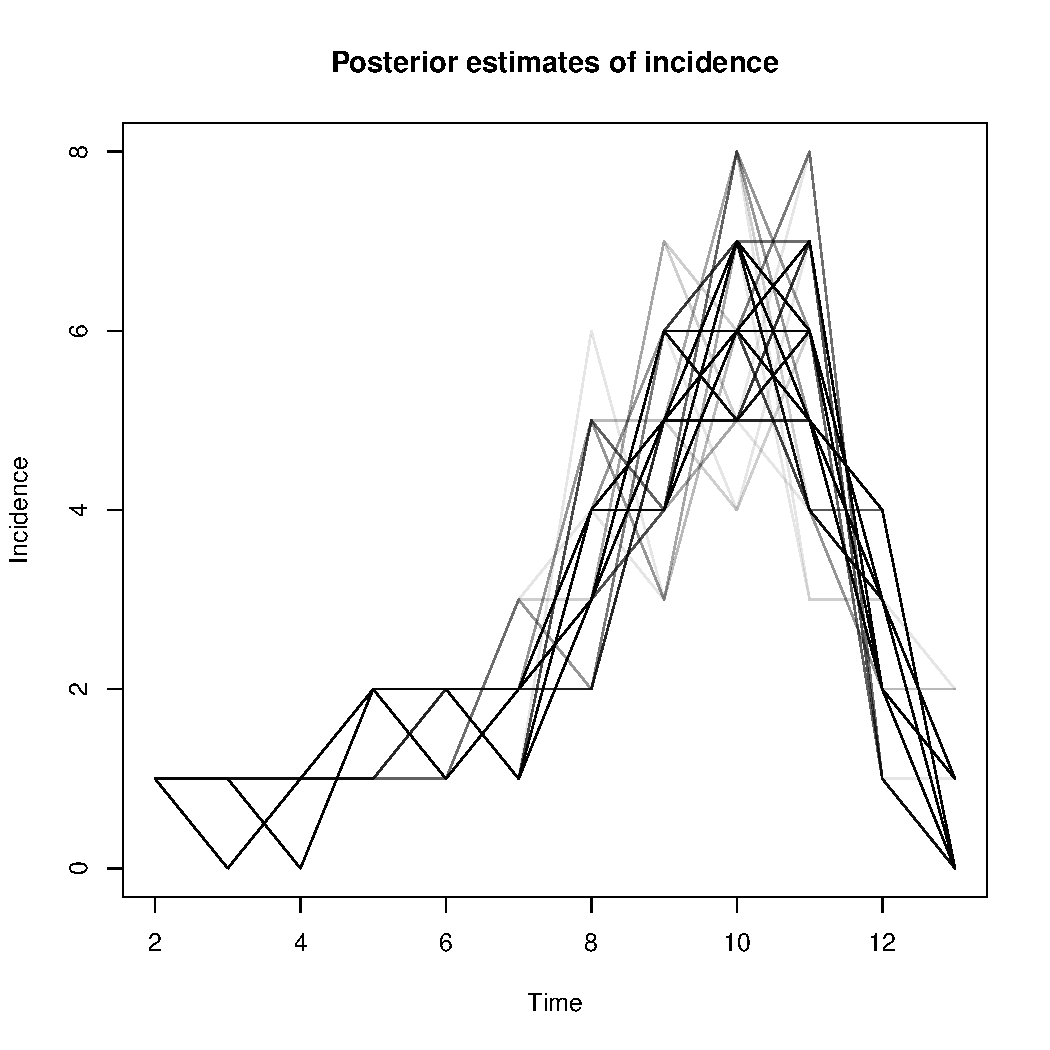
\includegraphics[width=.6\textwidth]{figs/unnamed-chunk-46} 

}



\end{knitrout}

Because a lot of these trajectories overlap, visualizing them all is a bit tricky.
\textit{ggplot2} will be helpful here.
We first reformat the data:
\begin{knitrout}
\definecolor{shadecolor}{rgb}{0.969, 0.969, 0.969}\color{fgcolor}\begin{kframe}
\begin{alltt}
\hlstd{x} \hlkwb{<-} \hlkwd{data.frame}\hlstd{(}\hlkwc{date}\hlstd{=}\hlkwd{as.vector}\hlstd{(}\hlkwd{row}\hlstd{(incid)),}
                \hlkwc{step}\hlstd{=}\hlkwd{as.vector}\hlstd{(}\hlkwd{col}\hlstd{(incid)),}
                \hlkwc{incidence}\hlstd{=}\hlkwd{as.vector}\hlstd{(incid))}
\hlkwd{head}\hlstd{(x)}
\end{alltt}
\begin{verbatim}
##   date step incidence
## 1    1    1         1
## 2    2    1         0
## 3    3    1         1
## 4    4    1         2
## 5    5    1         2
## 6    6    1         1
\end{verbatim}
\begin{alltt}
\hlstd{p} \hlkwb{<-} \hlkwd{ggplot}\hlstd{(}\hlkwc{data}\hlstd{=x,} \hlkwd{aes}\hlstd{(}\hlkwc{x}\hlstd{=date,} \hlkwc{y}\hlstd{=incidence))} \hlopt{+} \hlkwd{labs}\hlstd{(}\hlkwc{title}\hlstd{=}\hlstr{"Posterior estimates of incidence"}\hlstd{)}
\end{alltt}
\end{kframe}
\end{knitrout}


This is for a basic boxplot:
\begin{knitrout}
\definecolor{shadecolor}{rgb}{0.969, 0.969, 0.969}\color{fgcolor}\begin{kframe}
\begin{alltt}
\hlstd{p} \hlopt{+} \hlkwd{geom_boxplot}\hlstd{(}\hlkwd{aes}\hlstd{(}\hlkwc{x}\hlstd{=}\hlkwd{factor}\hlstd{(date)))}
\end{alltt}
\end{kframe}

{\centering 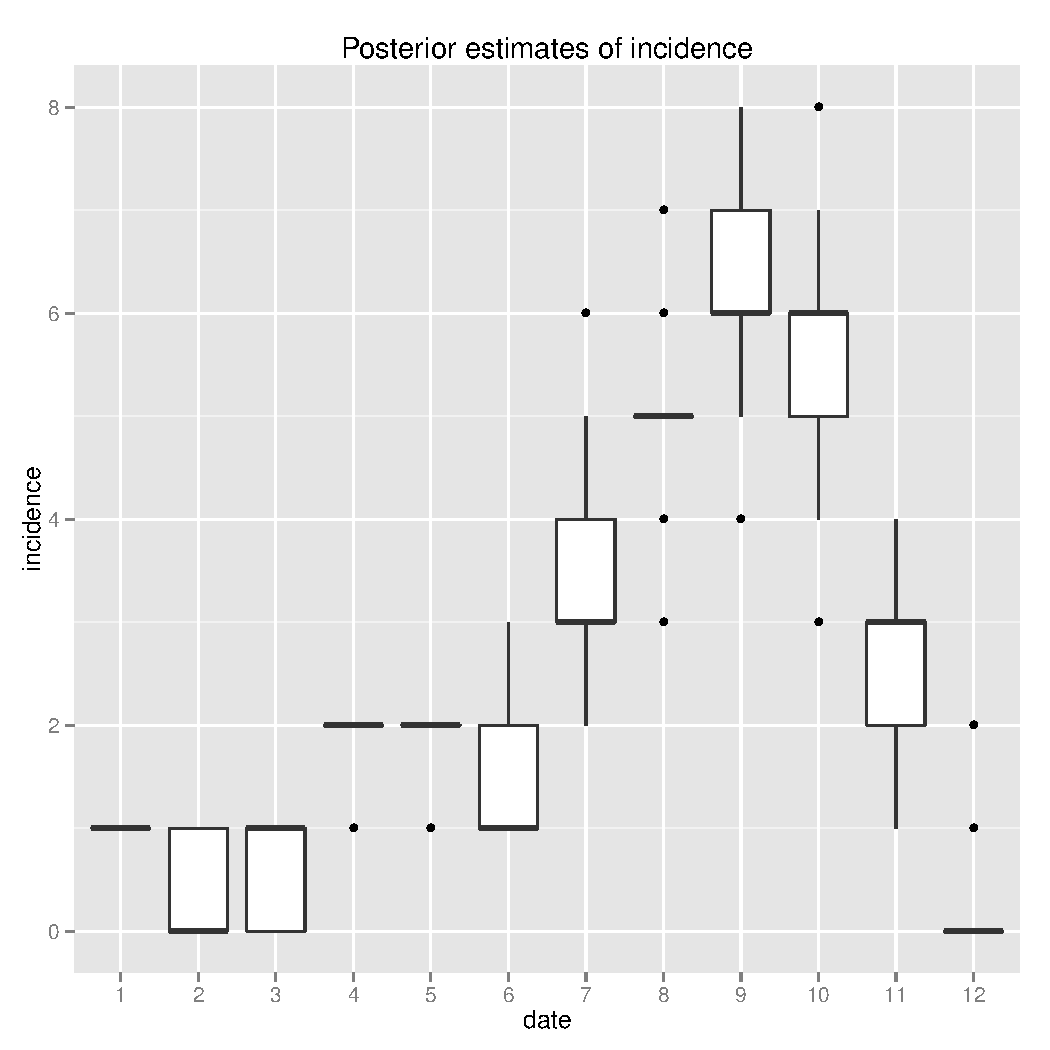
\includegraphics[width=.6\textwidth]{figs/unnamed-chunk-48} 

}



\end{knitrout}

\begin{knitrout}
\definecolor{shadecolor}{rgb}{0.969, 0.969, 0.969}\color{fgcolor}\begin{kframe}
\begin{alltt}
\hlstd{p} \hlopt{+} \hlkwd{geom_boxplot}\hlstd{(}\hlkwd{aes}\hlstd{(}\hlkwc{x}\hlstd{=}\hlkwd{factor}\hlstd{(date)))}
\end{alltt}
\end{kframe}

{\centering 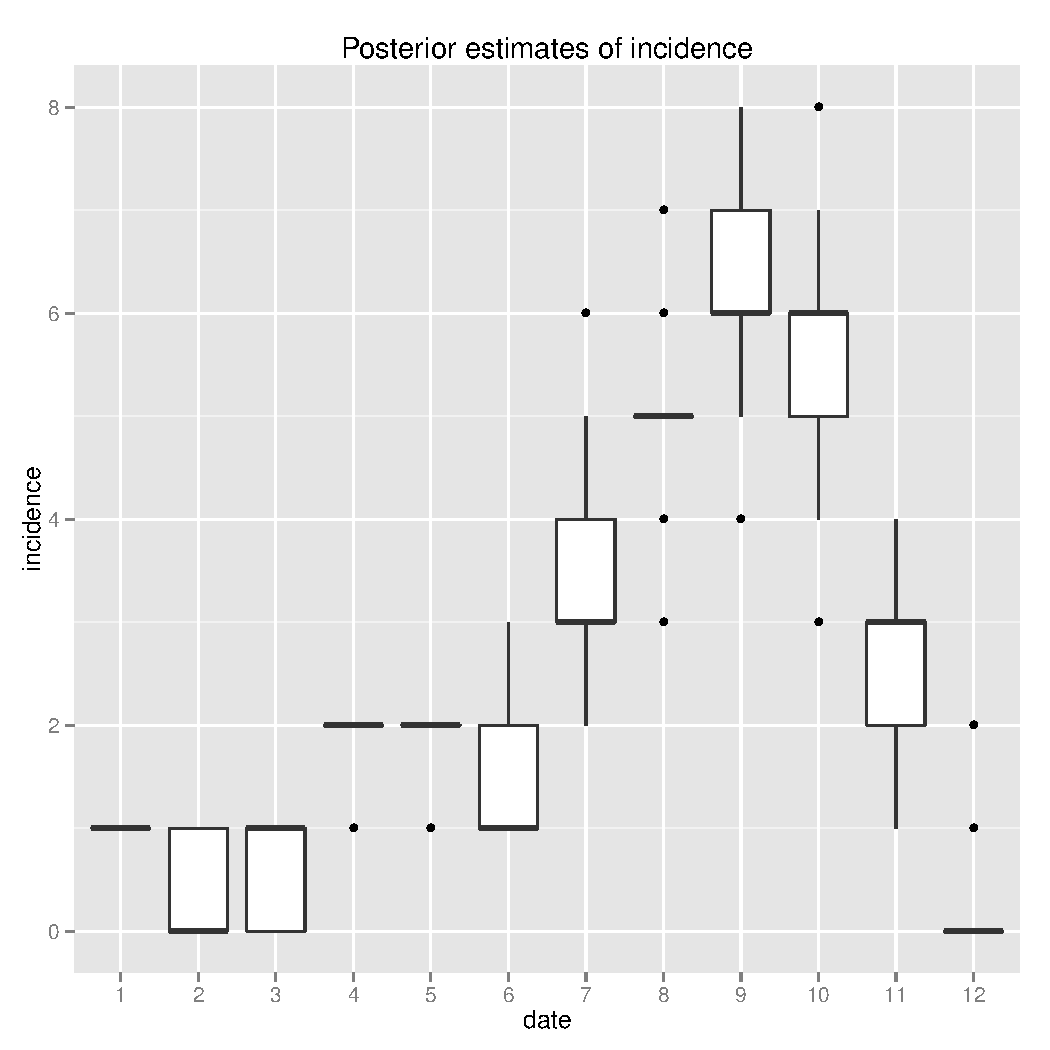
\includegraphics[width=.6\textwidth]{figs/unnamed-chunk-49} 

}



\end{knitrout}

A noisified version with a smoother can be obtained using:
\begin{knitrout}
\definecolor{shadecolor}{rgb}{0.969, 0.969, 0.969}\color{fgcolor}\begin{kframe}
\begin{alltt}
\hlkwd{library}\hlstd{(splines)}
\hlstd{p} \hlopt{+} \hlkwd{geom_jitter}\hlstd{(}\hlkwd{aes}\hlstd{(}\hlkwc{x}\hlstd{=}\hlkwd{factor}\hlstd{(date)),} \hlkwc{alpha}\hlstd{=}\hlnum{.2}\hlstd{)} \hlopt{+} \hlkwd{geom_smooth}\hlstd{(}\hlkwc{method}\hlstd{=lm,} \hlkwc{formula}\hlstd{=y}\hlopt{~}\hlkwd{ns}\hlstd{(x,}\hlnum{10}\hlstd{),} \hlkwc{size}\hlstd{=}\hlnum{1}\hlstd{)}
\end{alltt}
\end{kframe}

{\centering 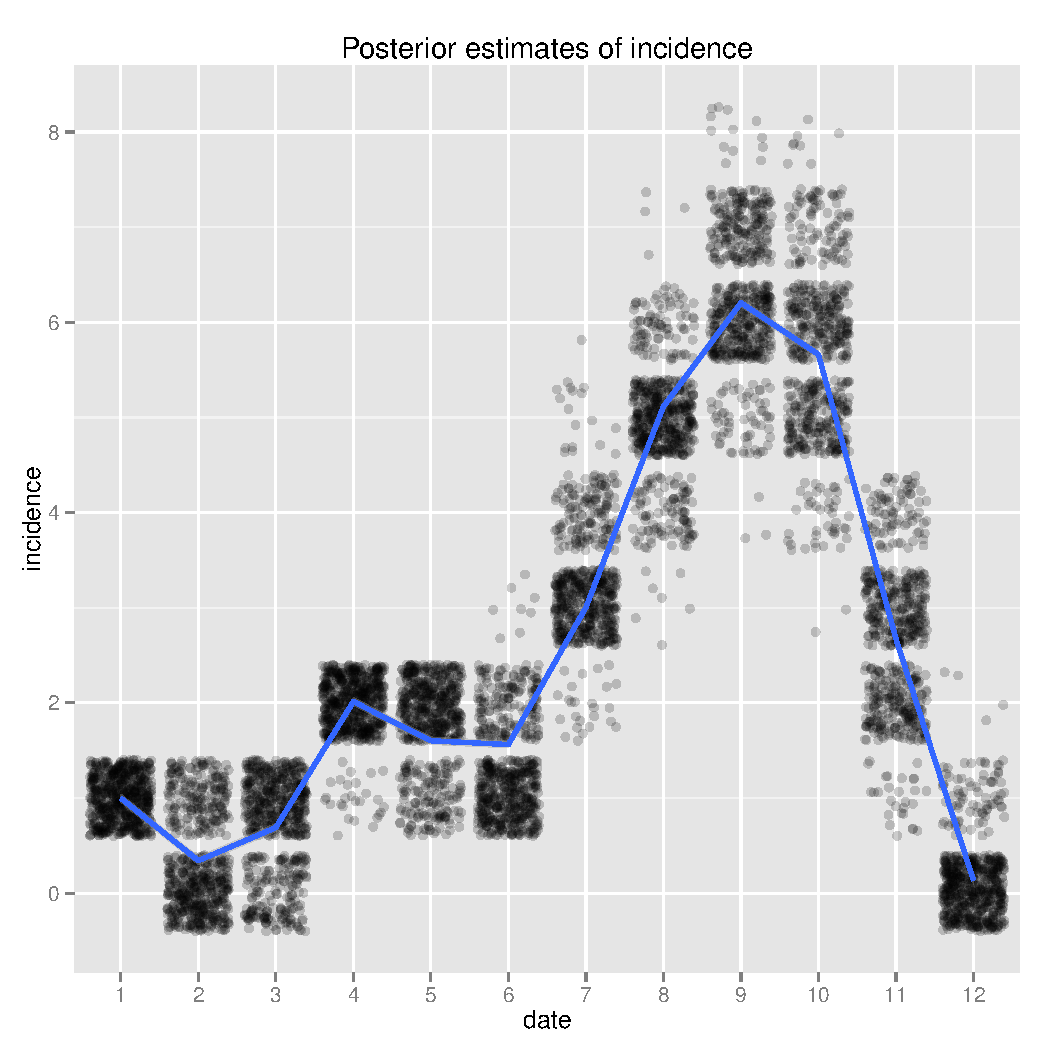
\includegraphics[width=.6\textwidth]{figs/unnamed-chunk-50} 

}



\end{knitrout}

However, it adds artifactual variation and may be best avoided here.

Another interesting option is offered by some density-based graphics:
\begin{knitrout}
\definecolor{shadecolor}{rgb}{0.969, 0.969, 0.969}\color{fgcolor}\begin{kframe}
\begin{alltt}
\hlstd{p} \hlopt{+} \hlkwd{geom_bin2d}\hlstd{()} \hlopt{+} \hlkwd{geom_smooth}\hlstd{(}\hlkwc{method}\hlstd{=lm,} \hlkwc{formula}\hlstd{=y}\hlopt{~}\hlkwd{ns}\hlstd{(x,}\hlnum{10}\hlstd{),} \hlkwc{size}\hlstd{=}\hlnum{1}\hlstd{)}
\end{alltt}
\end{kframe}

{\centering 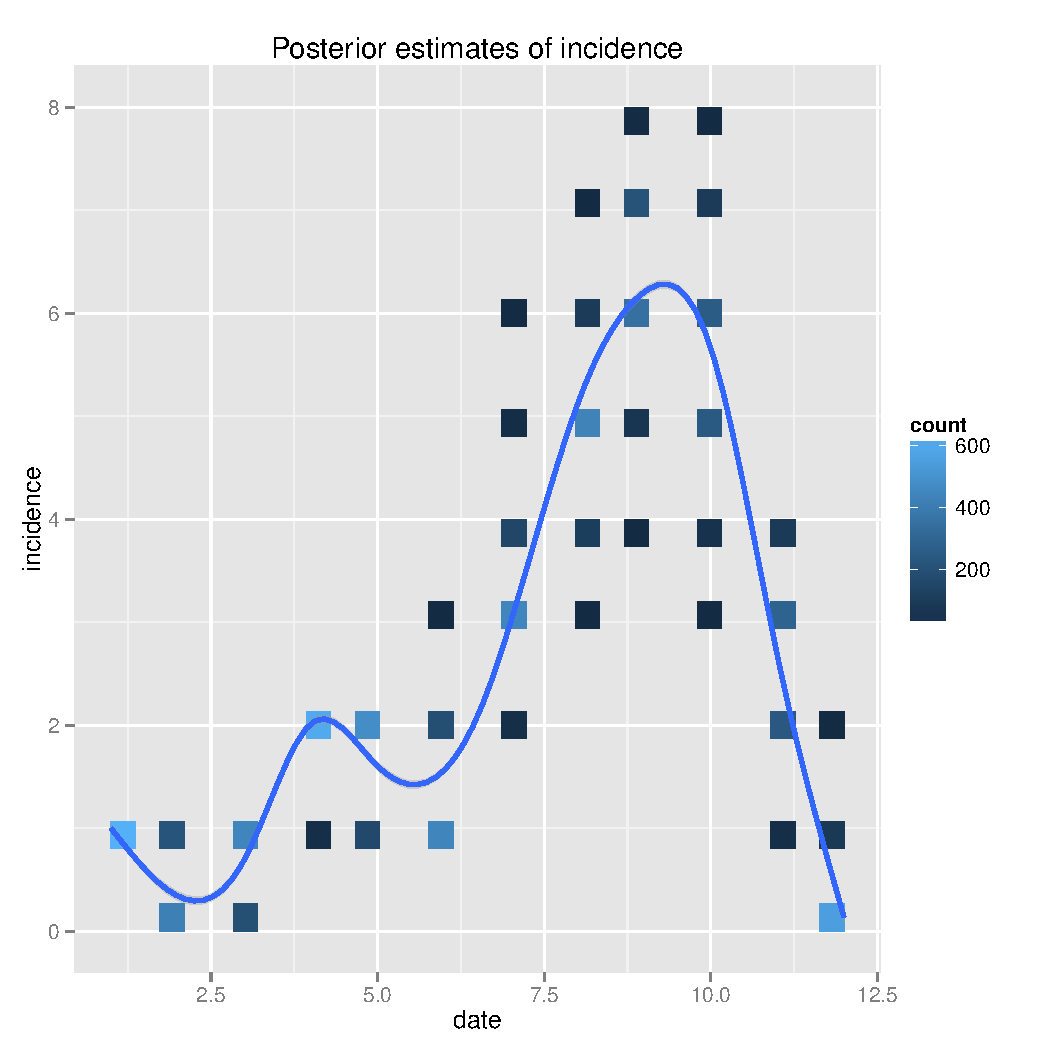
\includegraphics[width=.6\textwidth]{figs/unnamed-chunk-51} 

}



\end{knitrout}

or perhaps even better:
\begin{knitrout}
\definecolor{shadecolor}{rgb}{0.969, 0.969, 0.969}\color{fgcolor}\begin{kframe}
\begin{alltt}
\hlstd{p} \hlopt{+} \hlkwd{geom_hex}\hlstd{(}\hlkwc{bins}\hlstd{=}\hlnum{8}\hlstd{,} \hlkwc{alpha}\hlstd{=}\hlnum{.5}\hlstd{)} \hlopt{+} \hlkwd{geom_smooth}\hlstd{(}\hlkwc{colour}\hlstd{=}\hlstr{"purple4"}\hlstd{,}\hlkwc{size}\hlstd{=}\hlnum{2}\hlstd{)}
\end{alltt}


{\ttfamily\noindent\itshape\color{messagecolor}{\#\# geom\_smooth: method="{}auto"{} and size of largest group is >=1000, so using gam with formula: y \textasciitilde{} s(x, bs = "{}cs"{}). Use 'method = x' to change the smoothing method.}}\end{kframe}

{\centering 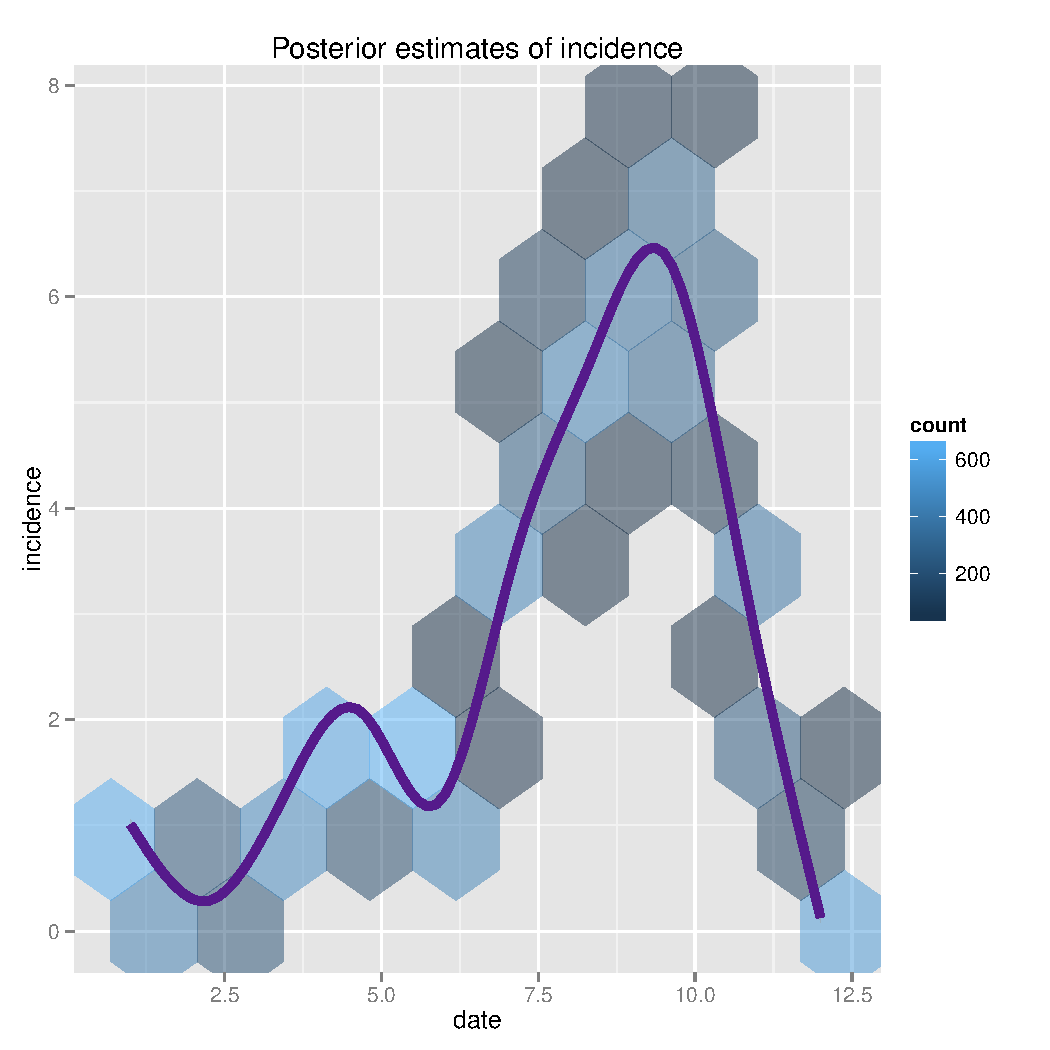
\includegraphics[width=.6\textwidth]{figs/unnamed-chunk-52} 

}



\end{knitrout}




Effective reproduction numbers over time can be obtained using \texttt{get.Rt}, and given identical outputs to \texttt{get.incid}.
Effective reproduction numbers per individuals can be obtained by \texttt{get.R}:
\begin{knitrout}
\definecolor{shadecolor}{rgb}{0.969, 0.969, 0.969}\color{fgcolor}\begin{kframe}
\begin{alltt}
\hlstd{R} \hlkwb{<-} \hlkwd{get.R}\hlstd{(res)}
\hlkwd{class}\hlstd{(R)}
\end{alltt}
\begin{verbatim}
## [1] "matrix"
\end{verbatim}
\begin{alltt}
\hlkwd{dim}\hlstd{(R)}
\end{alltt}
\begin{verbatim}
## [1] 640  30
\end{verbatim}
\begin{alltt}
\hlstd{R[}\hlnum{1}\hlopt{:}\hlnum{6}\hlstd{,}\hlnum{1}\hlopt{:}\hlnum{15}\hlstd{]}
\end{alltt}
\begin{verbatim}
##    1 2 3 4 5 6 7 8 9 10 11 12 13 14 15
## 42 1 1 1 2 3 2 3 2 2  2  2  0  4  0  0
## 43 1 1 1 2 4 2 3 0 2  2  2  1  4  0  0
## 44 1 1 1 2 3 2 3 2 2  2  2  0  4  0  0
## 45 1 1 1 2 5 2 3 0 2  1  2  0  4  0  0
## 46 1 1 1 2 4 2 3 1 2  2  2  0  4  0  0
## 47 1 1 1 2 4 2 3 0 2  2  2  1  4  0  0
\end{verbatim}
\end{kframe}
\end{knitrout}

\texttt{R} is a matrix of effective reproduction numbers with one column per individual and one row
for each retained step of the MCMC.
This information can be pooled to get a rough idea of the overall distribution of $R_i$:
\begin{knitrout}
\definecolor{shadecolor}{rgb}{0.969, 0.969, 0.969}\color{fgcolor}\begin{kframe}
\begin{alltt}
\hlkwd{table}\hlstd{(R)}
\end{alltt}
\begin{verbatim}
## R
##     0     1     2     3     4     5 
## 10498  2785  4070  1042   796     9
\end{verbatim}
\begin{alltt}
\hlkwd{table}\hlstd{(R)}\hlopt{/}\hlkwd{length}\hlstd{(R)}
\end{alltt}
\begin{verbatim}
## R
##         0         1         2         3         4         5 
## 0.5467708 0.1450521 0.2119792 0.0542708 0.0414583 0.0004687
\end{verbatim}
\begin{alltt}
\hlkwd{barplot}\hlstd{(}\hlkwd{table}\hlstd{(R)}\hlopt{/}\hlkwd{length}\hlstd{(R),} \hlkwc{xlab}\hlstd{=}\hlstr{"Number of secondary cases"}\hlstd{,}
        \hlkwc{main}\hlstd{=}\hlstr{"Posterior estimates of effective reproduction numbers (R)"}\hlstd{,} \hlkwc{ylab}\hlstd{=}\hlstr{"Frequency"}\hlstd{)}
\end{alltt}
\end{kframe}

{\centering 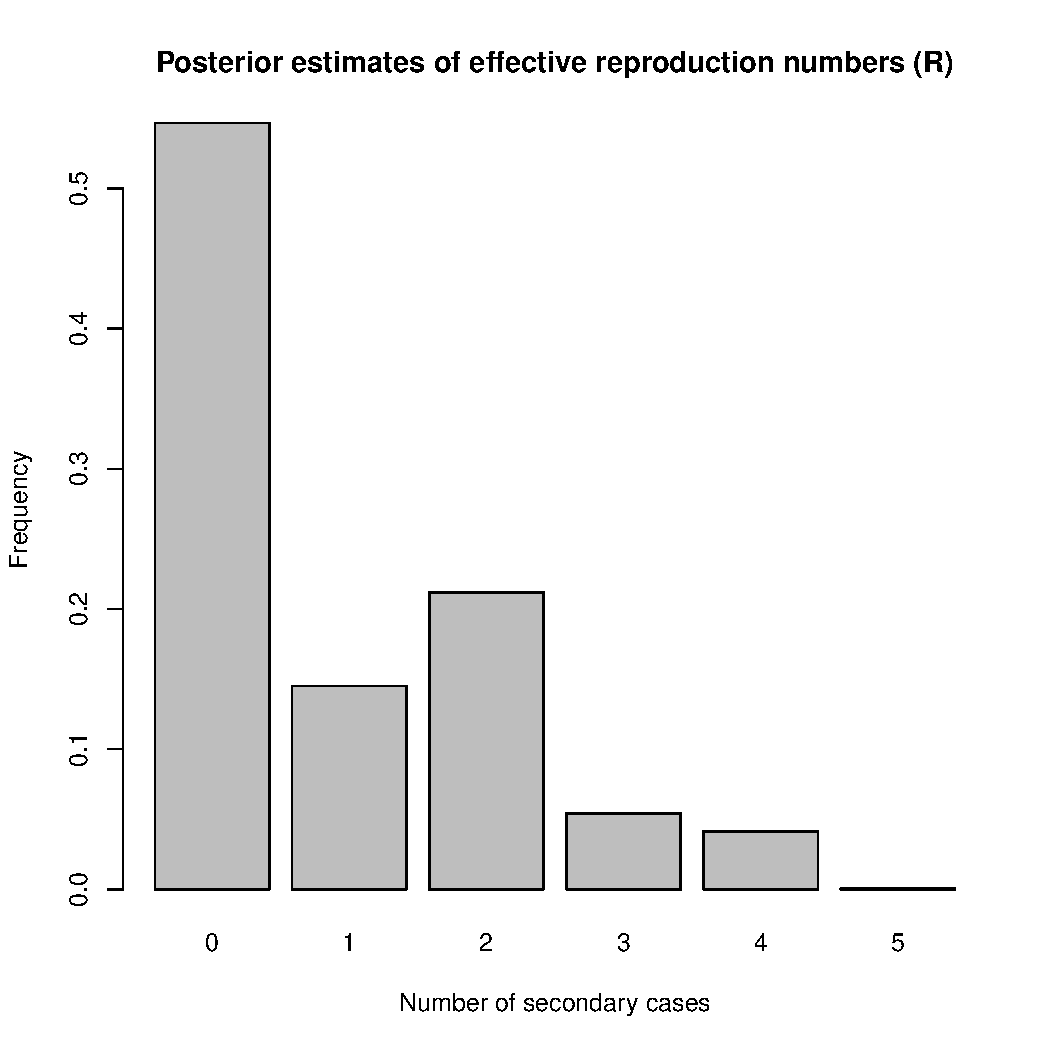
\includegraphics[width=.6\textwidth]{figs/unnamed-chunk-54} 

}



\end{knitrout}

And we can use \textit{ggplot2} to visualize the individual distributions:
\begin{knitrout}
\definecolor{shadecolor}{rgb}{0.969, 0.969, 0.969}\color{fgcolor}\begin{kframe}
\begin{alltt}
\hlstd{x} \hlkwb{<-} \hlkwd{data.frame}\hlstd{(}\hlkwc{case}\hlstd{=}\hlkwd{factor}\hlstd{(}\hlkwd{as.vector}\hlstd{(}\hlkwd{col}\hlstd{(R)),} \hlkwc{levels}\hlstd{=}\hlkwd{as.character}\hlstd{(}\hlnum{1}\hlopt{:}\hlnum{30}\hlstd{)),}\hlkwc{R}\hlstd{=}\hlkwd{as.vector}\hlstd{(R))}
\hlkwd{head}\hlstd{(x)}
\end{alltt}
\begin{verbatim}
##   case R
## 1    1 1
## 2    1 1
## 3    1 1
## 4    1 1
## 5    1 1
## 6    1 1
\end{verbatim}
\begin{alltt}
\hlkwd{tail}\hlstd{(x)}
\end{alltt}
\begin{verbatim}
##       case R
## 19195   30 0
## 19196   30 0
## 19197   30 0
## 19198   30 0
## 19199   30 0
## 19200   30 0
\end{verbatim}
\begin{alltt}
\hlstd{p} \hlkwb{<-} \hlkwd{ggplot}\hlstd{(}\hlkwc{data}\hlstd{=x,} \hlkwd{aes}\hlstd{(}\hlkwc{x}\hlstd{=case,} \hlkwc{y}\hlstd{=R))} \hlopt{+} \hlkwd{geom_boxplot}\hlstd{(}\hlkwd{aes}\hlstd{(}\hlkwc{colour}\hlstd{=case))}
\hlstd{p} \hlkwb{<-} \hlstd{p} \hlopt{+} \hlkwd{geom_boxplot}\hlstd{(}\hlkwd{aes}\hlstd{(}\hlkwc{colour}\hlstd{=case))} \hlopt{+} \hlkwd{guides}\hlstd{(}\hlkwc{colour}\hlstd{=}\hlnum{FALSE}\hlstd{)}
\hlstd{p} \hlopt{+} \hlkwd{labs}\hlstd{(}\hlkwc{title}\hlstd{=}\hlstr{"Posterior estimates of effective reproduction numbers"}\hlstd{)}
\end{alltt}
\end{kframe}

{\centering 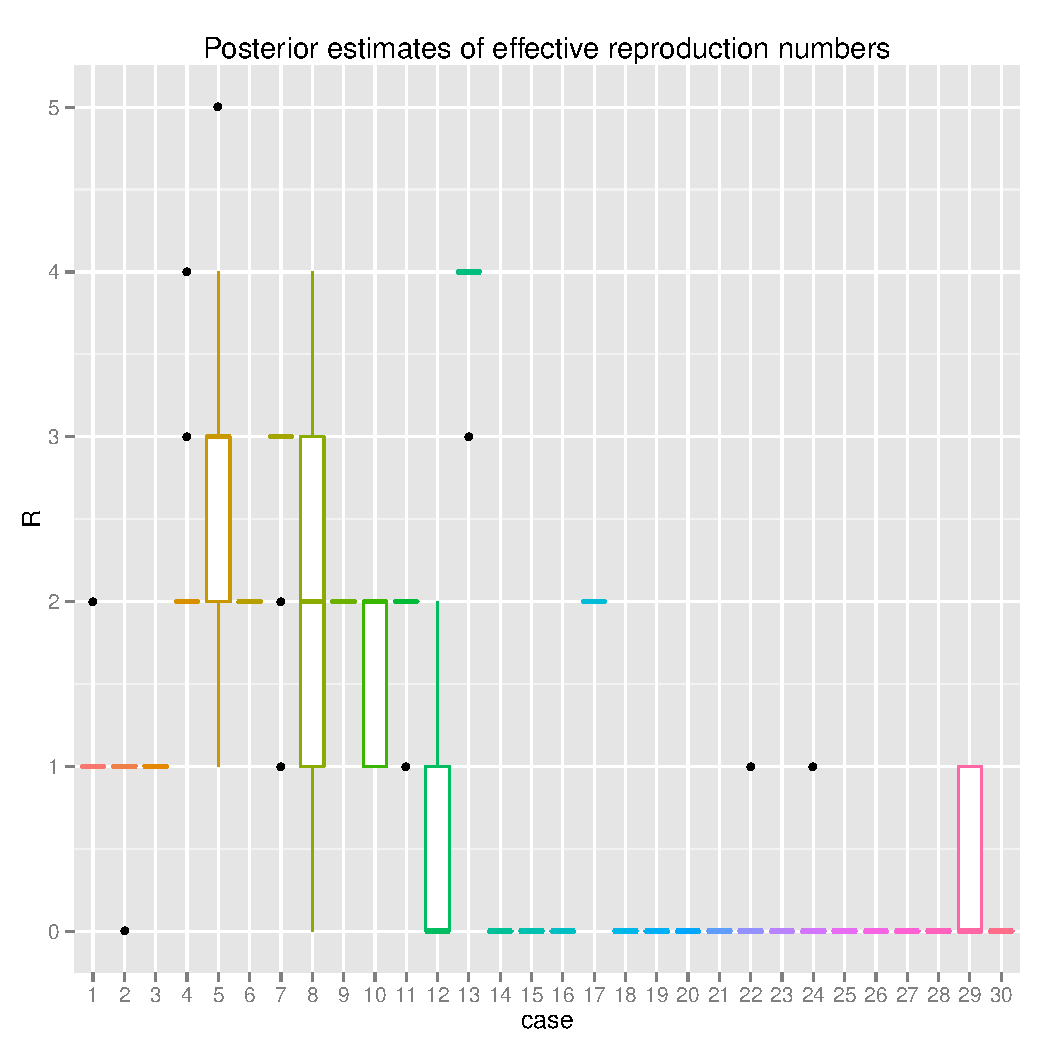
\includegraphics[width=.6\textwidth]{figs/unnamed-chunk-55} 

}



\end{knitrout}






%% %%%%%%%%%%%%%%%%%%%%%%%%%%%%%%%%%%%%%%%%%%%%%%%%%%%%
%% %%%%%%%%%%%%%%%%%%%%%%%%%%%%%%%%%%%%%%%%%%%%%%%%%%%%
%% \section{Advanced uses}
%% %%%%%%%%%%%%%%%%%%%%%%%%%%%%%%%%%%%%%%%%%%%%%%%%%%%%
%% %%%%%%%%%%%%%%%%%%%%%%%%%%%%%%%%%%%%%%%%%%%%%%%%%%%%



%% %%%%%%%%%%%%%%%%%%%%%%%%%%%%%%%%%%%%%%%%%%%%%%%%%%%%
%% \subsection{Fixing known ancestries}
%% %%%%%%%%%%%%%%%%%%%%%%%%%%%%%%%%%%%%%%%%%%%%%%%%%%%%



\end{document}
